\documentclass{jsarticle}


\usepackage{ascmac}
\usepackage[top=30truemm,bottom=30truemm,left=25truemm,right=25truemm]{geometry}
\usepackage{amsfonts}
\usepackage{amsmath,amssymb}
\usepackage[dvipdfmx]{graphicx}
\usepackage{cases}

\begin{document}

\title{集合と位相}
\author{nukui}
\date{\today}
\maketitle
\setcounter{tocdepth}{1}
\tableofcontents

\newpage

\part{集合と写像}
\section{集合とは}

%\begin{screen}
%\begin{description}
%\item[集合]\mbox{}\\ある特定の性質をそなえたものの集まりのこと。
%\item[元]\mbox{}\\集合を構成する一つ一つのもの。{\bf 要素}ともいう。
%\item[空集合]\mbox{}\\元を一つも含まない集合。
%\item[有限集合]\mbox{}\\元を有限個しか含まない集合および空集合。
%\item[無限集合]\mbox{}\\有限集合でない集合。
%\item[部分集合]\mbox{}\\二つの集合$A,B$について、$A$のどの元も$B$に含まれるとき、$A$は$B$の{\bf 部分集合}であるといい、$A\subset B$または$B\supset A$で表す。
%\item[真部分集]\mbox{}\\$A\subset B$かつ$A\neq B$であるとき、$A$を$B$の{\bf 真部分集合}であるという。
%\item[冪集合]\mbox{}\\集合$A$の部分集合の全体を$A$の{\bf 冪集合}といい、$\mathfrak{P}(A)$で表す。
%\item[集合族]\mbox{}\\どの元も集合であるような集合のこと。
%\end{description}
%\end{screen}

% 1.1
\subsection{}
\begin{enumerate}
\item 成り立つ。$\because$ Yに含まれる要素は全てXに含まれる。
\item 成り立つ。$\because$3はWに含まれるがZに含まれない。
\item 成り立つ。$\because$4はVに含まれるが、Yに含まれない。
\item 成り立たない。$\because$4はVに含まれるがXには含まれない。
\item 成り立たない。$\because$ 1はXに含まれるがWに含まれない。
\item 成り立たない。$\because$ Vの全ての要素はWに含まれる。
\item 成り立つ。$\because$ Vの全ての要素はZに含まれる。
\item 成り立つ。 $\because$ 3はXに含まれるがZに含まれない。
\item 成り立たない。 $\because$ Yに含まれる全ての要素はZに含まれる。
\item 成り立たない。$\because$ 3はWに含まれるがYには含まれない。
\end{enumerate}

%1.2
\subsection{}
\begin{enumerate}
\item D
\item B
\item C,\ E,\ F
\item B,D
\end{enumerate}

%1.3
\subsection{}
\begin{enumerate}
\item 成り立たない。
\item 成り立つ。
\item 成り立つ。
\item 成り立つ。
\item 成り立たない。
\item 成り立つ。
\end{enumerate}

%1.4
\subsection{}
集合Aが1個の元から成るとき、部分集合はAと$\emptyset$の2通り。よって$n=1$のとき、命題は成り立つ。\\
集合Aがn個の元から成り、その部分集合は全部で$2^n$個から成ると仮定する。
今、集合Aに元$x(x\notin A)$を一つ加え、$n+1$個の元から成る集合$B(B=A\cup\{x\})$を考える。
集合Bの部分集合は、
\begin{enumerate}
\item 集合Aの部分集合と一致。($2^n$個)
\item 集合Aの部分集合に元$x$を加えたものに一致。($2^n$個)
\end{enumerate}
のいずれかである。よって、集合Bの部分集合の個数は$2^n+2^n=2^{n+1}$個になる。以上より、すべての自然数$n$で命題は成り立つ。

%Section 2
\section{集合の演算}
%\begin{screen}
%\begin{description}
%\item[和集合]\mbox{}\\ある特定の性質をそなえたものの集まりのこと。
%\end{description}
%\end{screen}

\subsection{}
意味を考えれば、確かに成り立つことがわかる。

\subsection{}
\begin{enumerate}
\item
\begin{align*}
(A-B)\cup(A\cap B)&=\{x|x\in(A-B) またはx\in(A\cap B)\}\\
&=\{x|(x\in A かつ x\notin B) または (x\in A かつ x\in B)\}\\
&=\{x|x\in A かつ (x\notin B または x\in B)\}\\
&=\{x|x\in A\}\\
&=A
\end{align*}


\item
\begin{align*}
(A-B)\cup B &=\{x| x\in (A-B) または x \in B\}\\
&=\{ x | (x \in A かつ x\notin B) または x\in B \}\\
&=\{x | (x\in Aまたは x\in B) かつ( x\notin B または x\in B)\}\\
&=\{x| (x\in Aまたは x\in B)\}\\
&=A\cup B
\end{align*}


\item
\begin{align*}
B\cap(A-B)&=\{x|x\in B かつ x \in(A-B)\}\\
&=\{x|x\in B かつ( x \in A かつ x\notin B)\}\\
&=\emptyset
\end{align*}
\end{enumerate}

\subsection{}
\begin{enumerate}
\item
$A_1 \subset A$を仮定する。
\[x \in A_1 かつ x\notin B \Longrightarrow x\in A かつ x\notin B\]
なので、$x\in A_1-B$とすると、$x\in A-B$が示せる。つまり、$A_1-B \subset A-B$。
\item
$B_1 \subset B$を仮定する。
\[x \in A かつ x\notin B \Longrightarrow x\in A かつ x\notin B_1\]
なので、$x\in A-B$とすると、$x\in A-B_1$が示せる。つまり、$A-B \subset A-B_1$。
\end{enumerate}

\subsection{}
\begin{align*}
A-B&=\{x|x\in A かつ x\notin B\}\\
&=\{x|x\in A かつ (x\notin A または x\notin B)\}\\
&=\{x|x\in A かつ x\notin A\cap B\}\\\\
A&=\{x|x\in A\}
\end{align*}
なので、
\[A-B=A \Longleftrightarrow  A-B \supset A \Longleftrightarrow A\cap B = \emptyset\]
となり、$A-B=A$と、$A\cap B=\emptyset$が同値であることを示せた。

\subsection{}
\begin{enumerate}
\item
定義から、
\begin{align*}
A\cup B &= \{x | x\in A または x\in B\}\\
B&= \{x| x\in B\}
\end{align*}である。
ここで、$A\subset B$を仮定すると、$A\cup B = \{x | x\in B\}=B$となる。逆に、$A\cup B= B$を仮定すると、$A\cup B \subset B$より、$\forall x [ x\in A \Longrightarrow x\in B]$となるので、$A\subset B$。\\

\item
定義から、
\begin{align*}
A\cap B &= \{x | x\in A かつ x\in B\}\\
A&= \{x| x\in A\}
\end{align*}である。
ここで、$A\subset B$を仮定すると、$A\cap B = \{x | x\in A\}=A$となる。逆に、$A\cap B= A$を仮定すると、$ A\cap B \supset A$より、$\forall x [ x\in A \Longrightarrow x\in B]$となるので、$A\subset B$。\\

\item 定義から
\[A-B=\{x|x\in A かつ x\notin B\}\]
である。ここで、$A\subset B$を仮定すると、$\forall x [ x\in A \Longrightarrow x\in B]$なので、$A-B=\emptyset$が成り立つ。逆に、$A-B=\emptyset$を仮定すると、$\forall x [ x\in A \Longrightarrow x\in B]$になるので、$A\subset B$が成り立つ。\\

\item 定義から
\begin{align*}
A\cup (B-A)&=\{x|x\in A または x\in (B-A)\}\\
&=\{x|x\in A または (x\in B かつ x\notin A)\}\\
&=\{x|x\in A または x\in B\}\\
&= A\cup B
\end{align*}
よって、1と本質的に同じ問題なので、成立する。\\
\item 定義から
\begin{align*}
B-(B-A)&=\{x| x\in B かつ x\notin (B-A)\}\\
&=\{x| x\in B かつ (x\notin B または x\in A)\}\\
&=\{x| x \in B かつ x\in A\}\\
&= A\cap B
\end{align*}
よって、本質的に2と同じ問題なので、成立する。
\end{enumerate}


%% 2.6
\subsection{}
\begin{enumerate}
\item
\begin{align*}
(A\cup B) \cap (A\cup C) \cap(B\cup C) 
&=((A\cup B) \cap (A\cup C)) \cap(B\cup C) \\
&=((A\cup B) \cap A) \cup ((A\cup B) \cap C)) \cap(B\cup C) \\
&=(A\cup ((A\cup B) \cap C))\cap(B\cup C) \\
&=(A\cup ((A\cap C) \cup (B\cap C)))\cap(B\cup C) \\
&=(A \cup (B\cap C))\cap(B\cup C) \\
&=(A\cap(B\cup C)) \cup ((B\cap C)\cap (B\cup C))\\
&=((A\cap B)\cup (A\cap C)) \cup (B\cap C)\\
&=(A\cap B)\cup (A\cap C) \cup (B\cap C)
\end{align*}
\item 1の結果を用いる。
\begin{align*}
&\quad(A\cup B) \cap (A\cup C) \cap(A\cup D)\cap (B\cup C) \cap (B\cup D) \cap(C\cup D)\\
&=((A\cup B) \cap (A\cup C)\cap(B\cup C) )\cap((A\cup D)\cap (B\cup D)\cap(C\cup D))\\
&=((A\cap B)\cup (A\cap C) \cup (B\cap C))\cap (D\cup (A\cap B \cap C))\\
&=(((A\cap B)\cup (A\cap C) \cup (B\cap C))\cap D)\cup(((A\cap B)\cup (A\cap C) \cup (B\cap C))\cap(A\cap B \cap C))\\
&=((A\cap B\cap D)\cup (A\cap C\cap D) \cup (B\cap C\cap D))\cup (A\cap B \cap C)\\
&=(A\cap B \cap C)\cup(A\cap B\cap D)\cup(A\cap C\cap D)\cup (B\cap C\cap D)
\end{align*}
\end{enumerate}



%%%section 3%%%
\section{ド・モルガンの法則}
\subsection{}
\begin{enumerate}
\item
\begin{align*}
(A^c)^c&=(X-A)^c\\
&=\{x | x\in X - (X-A)\}\\
&=\{x\in X|x \notin X-A\}\\
&=\{x\in X|「x \in X かつ x \notin A」ではない\}\\
&=\{x\in X| x\notin X または x \in A\}\\
&=\{x\in X | x \in A\}\\
&= A
\end{align*}


\item
\[X^c = X-X =\{x| x\in X かつ x\notin X\}= \emptyset \]

\item
\[\emptyset^c = X-\emptyset = \{x | x\in X かつ x\notin \emptyset\} = X\]

\item
\begin{align*}
A\cup A^c &= \{x| x\in A または x\in A^c\}\\
&=\{x \in X | x \in A または x\notin A\}\\
&=X
\end{align*}

\item
\[A\cap A^c = (A^c)^c \cap A^c = (A^c \cup A)^c = X^c = \emptyset\]

\item
\begin{align*}
A-B&=\{x\in X | x\in A かつ x\notin B\}\\
&=\{x | x\in A かつ x\in X-B\}\\
&=\{x| x\in A かつ x\in B^c\}\\
&= A\cap B^c
\end{align*}

\item

\[(A^c\cap B^c)^c = (A^c)^c \cup (B^c)^c = A\cup B\]

\end{enumerate}

\subsection{}
\begin{enumerate}
\item
\begin{align*}
(A\cup B)-C &= \{x | x \in A\cup B かつ x\notin C\}\\
&=\{x| (x \in A または x\in B) かつ x\notin C\}\\
&=\{x| (x\in A かつ x\notin C) または (x\in B かつ x\notin C)\}\\
&=\{x| x\in A-C または x\in B-C\}\\
&=(A-C)\cup (B-C)
\end{align*}

\item
\begin{align*}
(A\cap B)-C &= \{x | x \in A\cap B かつ x\notin C\}\\
&=\{x| (x \in A かつ x\in B) かつ x\notin C\}\\
&=\{x| (x\in A かつ x\notin C) かつ (x\in B かつ x\notin C)\}\\
&=\{x| x\in A-C かつ x\in B-C\}\\
&=(A-C)\cap (B-C)
\end{align*}

\end{enumerate}

\subsection{}
\begin{enumerate}
\item
\begin{enumerate}
\item
\begin{align*}
A\circ B &= (A-B)\cup(B-A)\\
&=(B-A)\cup (A-B)\\
&= B\circ A
\end{align*}


\item
\begin{align*}
(A\circ B)\circ C &= ((A\circ B)-C) \cup (C-(A\circ B))\\
&=(((A-B)\cup(B-A))-C)\cup(C-((A-B)\cup(B-A)))\\
&=(((A-B)-C)\cup((B-A)-C))\cup((C-(A-B)) \cap (C - (B-A)))\\
&=((A-(B\cup C)) \cup (B-(A\cup C))) \cup (((C-A)\cup (C\cap B))\cap((C-B)\cup(C\cap A)))\\
&=((A-(B\cup C)) \cup (B-(A\cup C))) \cup \\
&\qquad((C-A)\cap(C-B)) \cup( (C-A)\cap(C\cap A))\cup((C\cap B)\cap(C-B))\cup((C\cap B)\cap(C\cap A))\\
&=((A-(B\cup C)) \cup (B-(A\cup C)))\cup((C-(A\cup B)) \cup \emptyset \cup \emptyset \cup (A\cap B \cap C))\\
&=(A-(B\cup C)) \cup (B-(C\cup A))\cup(C-(A\cup B)) \cup  (A\cap B \cap C)
\end{align*}

ここで、
\begin{align*}
C-(A-B)&=\{x|x\in C かつ x\notin (A-B)\}\\
&=\{x|x\in C かつ (x\notin A または x\in B))\}\\
&=\{x|(x\in C かつ x\notin A) または (x\in C かつx\in B)\}\\
&=(C-A)\cup(C\cap B)
\end{align*}
という結果を、3行目から4行目への変形で用いた。また、
\begin{align*}
(A\cup B)\cap(C\cup D)&=(A\cap (C\cup D))\cup(B\cap (C\cup D))\\
&=(A\cap C)\cup (A\cap D) \cup (B\cap C)\cup(B\cap D)
\end{align*}
という結果を、4行目から(5,6行目)への変形で用いた。\\
さて、$(A\circ B)\circ C=(A-(B\cup C)) \cup (B-(C\cup A))\cup(C-(A\cup B)) \cup  (A\cap B \cap C)$と変形できるので、$(A\circ B)\circ C$は、A,B,Cが全く同等で、任意の二つを入れ替えても同じ値であることがわかる。よって、$(A\circ B)\circ C=A\circ (B\circ C)$。
\item
\[A\circ A= (A-A)\cup (A-A)=\emptyset\]

\item
\[A\circ \emptyset = (A-\emptyset)\cup(\emptyset-A)=A\]

\end{enumerate}
\item
\begin{align*}
&\qquad A\circ X=B\\
&\iff (A\circ X)-B=\emptyset かつB-(A\circ X)=\emptyset\\
&\iff ((A\circ X)-B) \cup (B-(A\circ X))=\emptyset\\
&\iff ((A\circ X)\circ B)=\emptyset\\
&\iff ((A\circ B)\circ X)=\emptyset\\
&\iff ((A\circ B)-X)\cup (X-(A\circ B))=\emptyset\\
&\iff ((A\circ B)-X)=\emptyset かつ (X-(A\circ B))=\emptyset\\
&\iff A\circ B=X
\end{align*}
ここで、$((A\circ X)\circ B)=\emptyset\iff((A\circ B)\circ X)=\emptyset$という変形には、1の結果を用いた。
以上より、集合A,Bを任意に与えたとき、$A\circ X=B$を満足する集合$X$が$A\circ B$と表せるので、$X$はただ一つ存在することが示せた。
\end{enumerate}

\section{直積集合}
\subsection{}
\begin{enumerate}
\item
\begin{align*}
A\times(B\cup C)&= \{(x,y)|x\in A かつy\in(B\cup C)\}\\
&=\{(x,y)|(x\in A かつ y\in B)または(x\in A かつ y\in C)\}\\
&=\{(x,y)|(x,y)\in (A\times B) または (x,y)\in(A\times C)\}\\
&=(A\times B) \cup (A\times C)
\end{align*}

\item
\begin{align*}
A\times(B\cap C)&= \{(x,y)|x\in A かつy\in(B\cap C)\}\\
&=\{(x,y)|(x\in A かつ y\in B)かつ(x\in A かつ y\in C)\}\\
&=\{(x,y)|(x,y)\in (A\times B) かつ (x,y)\in(A\times C)\}\\
&=(A\times B) \cap (A\times C)
\end{align*}

\item
\begin{align*}
(A\cup B)\times C&=\{(x,y)|x\in (A\cup B) かつ y\in C\}\\
&=\{(x,y)|(x\in A かつ y\in C)または(x\in B かつ y\in C)\}\\
&=\{(x,y)|(x,y)\in A\times C または (x,y)\in B \times C\}\\
&=(A\times C)\cup(B\times C)
\end{align*}

\item
\begin{align*}
(A\cap B)\times C&=\{(x,y)|x\in (A\cap B) かつ y\in C\}\\
&=\{(x,y)|(x\in A かつ y\in C)かつ(x\in B かつ y\in C)\}\\
&=\{(x,y)|(x,y)\in A\times C かつ (x,y)\in B \times C\}\\
&=(A\times C)\cap(B\times C)
\end{align*}

\end{enumerate}

\subsection{}
\begin{align*}
(X\times Y)-(A\times B)&=\{(s,t)|(s,t)\in(X\times Y)かつ(s,t)\notin(A\times B)\}\\
&=\{(s,t)|(s\in(X-A) かつ t\in Y)\\
&\qquad\qquad または(s\in X かつ t\in(Y-B))\}\\
&=\{(s,t)|(s,t)\in ((X-A)\times Y) または (s,t)\in(X\times (Y-B))\}\\
&=((X-A)\times Y)\cup(X\times(Y-B))
\end{align*}

\section{写像}
\subsection{}
\begin{enumerate}
\item
\[(f\circ g)(x)=f(x^2+1)=x^2+3\]
\item
\[(g\circ f)(x)=g(x+2)=(x+2)^2+1=x^2+4x+5\]
\item
\[(f\circ f)(x)=f(x+2)=x+4\]
\item
\[(g\circ g)(x)=g(x^2+1)=(x^2+1)^2+1=x^4+2x^2+2\]
\end{enumerate}

\subsection{}
\begin{enumerate}
\item
\begin{align*}
(\bigcup_{\lambda\in\Lambda}A_\lambda)\cap B&=\{x| x\in\bigcup_{\lambda\in\Lambda}A_\lambda かつ x\in B\}\\
&=\{x|\exists \lambda\in\Lambda[x\in A_{\lambda}]かつx\in B\}\\
&=\{x|\exists \lambda\in\Lambda[x\in A_{\lambda} かつ x\in B]\}\\
&=\{x|\exists \lambda\in\Lambda[x\in (A_{\lambda} \cap B)]\}\\
&=\bigcup_{\lambda\in\Lambda}(A_{\lambda}\cap B)
\end{align*}

\item
\begin{align*}
(\bigcap_{\lambda\in\Lambda}A_\lambda)\cup B&=\{x| x\in\bigcap_{\lambda\in\Lambda}A_\lambda または x\in B\}\\
&=\{x|\forall \lambda\in\Lambda[x\in A_{\lambda}]またはx\in B\}\\
&=\{x|\forall \lambda\in\Lambda[x\in A_{\lambda} または x\in B]\}\\
&=\{x|\forall \lambda\in\Lambda[x\in (A_{\lambda} \cup B)]\}\\
&=\bigcap_{\lambda\in\Lambda}(A_{\lambda}\cup B)
\end{align*}
\end{enumerate}

\subsection{}
\begin{enumerate}
\item
\begin{align*}
(\bigcup_{\lambda\in\Lambda}A_{\lambda})^c&=(X-\bigcup_{\lambda\in\Lambda}A_{\lambda})\\
&=\{x|x\in X かつ 「\exists\lambda\in\Lambda [x\in A_\lambda]ではない」\}\\
&=\{x|x\in X かつ \forall \lambda\in\Lambda[x\notin A_\lambda]\}\\
&=\{x|\forall \lambda\in\Lambda[x\in X かつ x\notin A_\lambda]\}\\
&=\bigcap_{\lambda\in\Lambda}(A_\lambda^c)
\end{align*}

\item
\begin{align*}
(\bigcap_{\lambda\in\Lambda}A_{\lambda})^c&=(X-\bigcap_{\lambda\in\Lambda}A_{\lambda})\\
&=\{x|x\in X かつ 「\forall\lambda\in\Lambda [x\in A_\lambda]ではない」\}\\
&=\{x|x\in X かつ \exists \lambda\in\Lambda[x\notin A_\lambda]\}\\
&=\{x|\exists \lambda\in\Lambda[x\in X かつ x\notin A_\lambda]\}\\
&=\bigcup_{\lambda\in\Lambda}(A_\lambda^c)
\end{align*}
\end{enumerate}

\subsection{}
\begin{enumerate}
\item
\begin{align*}
f(\bigcup_{\lambda\in\Lambda}A_\lambda)&=\{y\in Y| \exists x \in(\bigcup_{\lambda\in\Lambda}A_\lambda)[f(x)=y]\} \\
&=\{y\in Y|\exists \lambda \in \Lambda[\exists x \in A_\lambda[f(x)=y]]\}\\
&=\{y\in Y|\exists \lambda \in \Lambda[y\in f(A_\lambda)]\}\\
&=\bigcup_{\lambda \in \Lambda}f(A_\lambda)
\end{align*}
\item
\[y\in f(\bigcap_{\lambda\in\Lambda}A_\lambda)\]と仮定すると、\[\exists x \in(\bigcap_{\lambda\in\Lambda}A_\lambda)[f(x)=y]\]が言える。これは、
\[\exists x \in X[\forall \lambda \in \Lambda[x \in A_\lambda かつ f(x)=y]]\]
と同値。このとき、
\[\forall \lambda \in \Lambda[\exists x \in A_\lambda [f(x)=y]]\]
がいえる\footnote{逆は必ずしも真ではない。つまり$\forall \lambda \in \Lambda[\exists x \in A_\lambda [f(x)=y]]$だからといって、$\exists x \in X[\forall \lambda \in \Lambda[x \in A_\lambda かつ f(x)=y]]$はいえない。}ので、
\[y\in \bigcap_{\lambda\in\Lambda}f(A_{\lambda})\]

\item
\begin{align*}
f^{-1}(\bigcup_{\mu\in M}B_{\mu})&=\{x\in X| f(x) \in(\bigcup_{\mu\in M}B_{\mu})\} \\
&=\{x\in X| \exists \mu \in M [f(x) \in B_{\mu}]\}\\
&=\{x\in X| \exists \mu \in M [x\in f^{-1}(B_{\mu})]\}\\
&=\bigcup_{\mu\in M}f^{-1}(B_{\mu})
\end{align*}

\item
\begin{align*}
f^{-1}(\bigcap_{\mu\in M}B_{\mu})&=\{x\in X|f(x)\in(\bigcap_{\mu\in M}B_{\mu}) \}\\
&=\{x\in X | \forall \mu\in M[f(x)\in B_{\mu}]\}\\
&=\{x\in X | \forall \mu\in M [x\in f^{-1}(B_{\mu})]\}\\
&=\bigcap_{\mu\in M}f^{-1}(B_{\mu})
\end{align*}
\end{enumerate}

\subsection{}
$n=2$のとき
\[A_1 \cup A_2 =A_1\cup A_2\]
となり、主張は正しい。
$n=m$のとき、主張が正しいと仮定する。つまり、
\[\bigcap_{1\leqq i<j\leqq m}(A_i \cup A_j )=\bigcup_{1\leqq i\leqq m}(A_1\cap \cdots\cap A_{i-1}
\cap A_{i+1} \cap \cdots \cap A_{m})\]
が成り立つと仮定すると、
\begin{align*}
&\quad\bigcap_{1\leqq i<j\leqq m+1}(A_i \cup A_j )\\
&=(\bigcap_{1\leqq i<j\leqq m}(A_i \cup A_j ))\cap (\bigcap_{1\leqq i\leqq m}(A_{i}\cup A_{m+1}))\\
&=(\bigcup_{1\leqq i\leqq m}(A_1\cap \cdots\cap A_{i-1}\cap A_{i+1} \cap \cdots \cap A_{m}))\cap((\bigcap_{1\leqq i\leqq m}A_{i})\cup A_{m+1})\\
&=\bigcup_{1\leqq i\leqq m}(A_1\cap \cdots\cap A_{i-1}\cap A_{i+1} \cap \cdots \cap A_{m}\cap((\bigcap_{1\leqq i\leqq m}A_{i})\cup A_{m+1}))\\
&=(\bigcap_{1\leqq i\leqq m}A_{i})\cup(\bigcup_{1\leqq i\leqq m}(A_1\cap \cdots\cap A_{i-1}\cap A_{i+1} \cap \cdots \cap A_{m+1}))\\
&=\bigcup_{1\leqq i\leqq m+1}(A_1\cap \cdots\cap A_{i-1}
\cap A_{i+1} \cap \cdots \cap A_{m+1})
\end{align*}
となり、$n=m+1$のときも成り立つ。以上より、$n\geqq 2$のすべての自然数$n$で主張は成り立つ。


\subsection{}
\begin{enumerate}
\item
\[x\in\liminf_{n\to\infty}E_{n}\]
と仮定すると、定義より
\[\exists k \geqq 1 [\forall n\geqq k[x\in E_{n}]]\]
が成り立つ。よって、
\[\forall s \geqq 1[\exists k\geq 1[(m \geq k かつ m\geq s)\Longrightarrow x\in E_{m}]]\]
となるので、
\[\forall s \geq 1[\exists m\geq s[x\in E_{m}]]\]
定義より、\[x\in\limsup_{n\to\infty}E_{n}\]

\item
\[x\in\liminf_{n\to\infty}A_{n}\]
と仮定すると、定義より、
\[\exists k\geqq 1[\forall n\geqq k[x\in A_{n}]]\]
ここで、$\forall n\in N[A_n \subset B_n]$なので、
\[\exists k\geqq 1[\forall n\geqq k[x\in B_{n}]]\]
が言える。結局、
\[x\in\liminf_{n\to\infty}B_{n}\]
$\limsup$の場合も同様に示せる。
\item
\begin{align*}
\limsup_{n\to\infty}(A_{n}\cup B_{n})&=\{x|\forall k\geqq 1[\exists n\geqq k[x\in(A_{n}\cup B_{n})]]\}\\
&=\{x|\forall k\geqq 1[\exists n\geqq k[x\in A_{n} または x\in B_{n}]]\}\\
&=\{x|\forall k\geqq 1[(\exists n\geqq k[x\in A_{n}]) または (\exists m \geqq k[x\in B_{m}])]\}\\
&=\{x|(\forall k\geqq 1[\exists n\geqq k[x\in A_{n}]]) または (\forall s\geqq 1[\exists m \geqq s[x\in B_{m}]])\}\\
&=\{x|x\in(\limsup_{n\to\infty}A_{n})\cup (\limsup_{n\to\infty}B_{n})\}\\
&=(\limsup_{n\to\infty}A_{n})\cup (\limsup_{n\to\infty}B_{n})
\end{align*}
ここで、$3行目\Longrightarrow4行目$を示すには、「4行目でない$\Longrightarrow$3行目でない」を示せば良い。
\item
\begin{align*}
\liminf_{n\to\infty}(A_{n}\cap B_{n})&=\{x|\exists k\geqq 1[\forall n\geqq k[x\in(A_{n}\cap B_{n})]]\}\\
&=\{x|\exists k\geqq 1[\forall n\geqq k[x\in A_{n} かつ x\in B_{n}]]\}\\
&=\{x|\exists k\geqq 1[(\forall n\geqq k[x\in A_{n}]) かつ (\forall m \geqq k[x\in B_{m}])]\}\\
&=\{x|(\exists k\geqq 1[\forall n\geqq k[x\in A_{n}]]) かつ (\exists s\geqq 1[\forall m \geqq s[x\in B_{m}]])\}\\
&=\{x|x\in(\liminf_{n\to\infty}A_{n})\cap (\liminf_{n\to\infty}B_{n})\}\\
&=(\liminf_{n\to\infty}A_{n})\cap (\liminf_{n\to\infty}B_{n})
\end{align*}
\end{enumerate}
\subsection{}
\begin{enumerate}
\item
 \\各$n\in N$に対して、$E_{n}\subset E_{n+1}$のとき、$\bigcap_{n=k}^{\infty}E_{n}=E_{k}$なので、
\begin{align*}
\lim_{n\to\infty}E_{n}&=\bigcup_{k=1}^{\infty}\bigcap_{n=k}^{\infty}E_{n}\\
&=\bigcup_{k=1}^{\infty}E_{k}
\end{align*}
\item
 \\各$n\in N$に対して、$E_{n}\supset E_{n+1}$のとき、$\bigcup_{n=k}^{\infty}E_{n}=E_{k}$なので、
\begin{align*}
\lim_{n\to\infty}E_{n}&=\bigcap_{k=1}^{\infty}\bigcup_{n=k}^{\infty}E_{n}\\
&=\bigcap_{k=1}^{\infty}E_{k}
\end{align*}

\end{enumerate}
\subsection{}
\begin{enumerate}
\item
問5.6(3)より、
\[\lim_{n\to\infty}(A_n \cup B_n)=\limsup_{n\to\infty}(A_n \cup B_n)=\limsup_{n\to\infty}A_n \cup \limsup_{n\to\infty}B_n=\lim_{n\to\infty}A_n\cup\lim_{n\to\infty}B_n\]
\item
問5.6(4)より、
\[\lim_{n\to\infty}(A_n \cap B_n)=\liminf_{n\to\infty}(A_n \cap B_n)=\liminf_{n\to\infty}A_n \cap \liminf_{n\to\infty}B_n=\lim_{n\to\infty}A_n\cap\lim_{n\to\infty}B_n\]
\end{enumerate}

\subsection{}
\begin{enumerate}
\item
\begin{align*}
\limsup_{n\to\infty}E_{n}&=\{x|\forall k\geqq 1[\exists n \geqq k[x\in E_{n}]]\}\\
&=\{x|\forall k\geqq 1[\exists n[2n-1 \geqq k かつ (x\in E_{2n} または x\in E_{2n-1})]]\}\\
&=\{x|\forall k\geqq 1[\exists n [2n-1 \geqq k かつ (x \in A または x\in B)]]\}\\
&=\{x|x\in A または x\in B\}\\
&=A\cup B
\end{align*}
\item
\begin{align*}
\liminf_{n\to\infty}E_{n}&=\{x|\exists k\geqq 1[\forall n \geqq k[x\in E_{n}]]\}\\
&=\{x|\exists k\geqq 1[\forall n [2n-1\geqq k \Longrightarrow (x\in E_{2n-1}かつx\in E_{2n})]]\}\\
&=\{x|\exists k\geqq 1[\forall n [2n-1\geqq k \Longrightarrow (x\in A かつx\in B)]]\}\\
&=\{x|x\in A かつx\in B\}\\
&=A\cap B
\end{align*}
\end{enumerate}



\part{濃度の大小と二項関係}
\section{全射・単射}
\subsection{}
\begin{enumerate}
\item
$f:A\to B$が単射と仮定する。
\begin{enumerate}
\item
\[y\in f(A_1)\cap f(A_2)\]
と仮定すると、$y=f(x)$となる$x$が存在し、$x\in A_1$かつ$x\in A_2$となる。(もしも$x\notin A_1$または$x\notin A_2$とすると、$f$が単射でないことになってしまう。)よって、
\[y\in f(A_1 \cap A_2)\]\\
\item
任意の$x$について$f^{-1}(f(x))=x$なので、$x\in f^{-1}(f(A_1))$と仮定すると$x\in A_1$である。\\
\item
\[y\in f(A_1 - A_2)\]
と仮定すると、$f(x)=y$となる$x\in A_1 - A_2$がただ一つ存在する。よって、$y\in f(A_1)$かつ$y\notin f(A_2)$である。
\end{enumerate}
\item
\[f:A\to B\]
が全射とする。$y\in B_1$と仮定すると、$f(x)=y$となる$x\in f^{-1}(B_1)$が存在する。よって、$y\in f(f^{-1}(B_1))$。
\end{enumerate}
\subsection{}
\begin{enumerate}
\item
$g\circ f$が単射と仮定すると、
\[\forall x_1, x_2\in A[x_1\neq x_2 \Longrightarrow g\circ f(x_1)\neq g\circ f(x_2) ]\]
ここで、$f(x_1)=f(x_2)\Longrightarrow g\circ f(x_1)=g\circ f(x_2)$なので、
\[\forall x_1, x_2\in A[x_1\neq x_2 \Longrightarrow f(x_1)\neq f(x_2) ]\]
が成り立つ。よって、$f$は単射である。
\item
$g\circ f$が全射と仮定すると、
\[\forall c\in C[\exists a\in A[g\circ f(a)=c]]\]
ここで、$\forall a\in A[f(a)\in B]$なので、
\[\forall c\in C[\exists b\in B[g(b)=c]]\]
\end{enumerate}

\subsection{}
\[\forall n\in \mathbb{N}[\forall x\in X[h^n(x)\neq x]]\]
と仮定すると、任意の$n\in\mathbb{N}, x\in X$について、$x,h(x),h^2(x),\dots,h^n(x)$は互いに異なる値となる。つまり、$h:X\to X$より、Xに無限個の元が存在することになってしまい、矛盾。
よって、
\[\exists n\in \mathbb{N}[\exists x\in X[h^n(x)= x]]\]

\subsection{}
たとえば、$y=\frac{d-c}{b-a}x+\frac{bc-ad}{b-a}$は、条件を満たす。

\subsection{}
$f$は全射かつ単射である。実際、
\[
\begin{cases}
y=\frac{1}{2}ならば、x=0\\
y=\frac{1}{2^n}\quad(n=2,3,\dots)ならば、x=4y\\
それ以外ならば、x=y
\end{cases}
\]
というように、任意の$y$に関して、$f(x)=y$となる$x$がただ一つ存在するので、$f$は全単射。

\subsection{}
以下のように定義された写像$f$は条件を満たす。
\[f(x)=
\begin{cases}
1,  \qquad x=0\\
\frac{x}{2}, \qquad x=\frac{1}{2^n}(n=0,1,2,\dots)\\
x, \qquad x\neq 0, \frac{1}{2^n}(n=0,1,2,\dots)
\end{cases}
\]



\section{濃度の大小}
\subsection{}
\begin{enumerate}
\item
恒等写像$1_{A}:A\to A$は全単射である。
\item
$A\sim B$と仮定すると、全単射の写像$f:A\to B$が存在する。ここで、$f$の逆写像$f^{-1}$も全単射である。よって、$B\sim A$。
\item
$A\sim B$かつ$B\sim C$と仮定すると、全単射の写像$f:A\to B$と、$g:B\to C$が存在する。ここで、$g\circ f:A\to C$も全単射である。よって、$A\sim C$。
\end{enumerate}

\subsection{}
$F(A\times B, C)$の元である写像$f:A\times B\to C$が与えられた時、$F(A,F(B,C))$の元である写像$g:A\to F(B,C)$を以下のように定義することで対応させるとする。
\[(g(a))(b)=f(a,b)\]
このとき、任意の$g:A\to F(B,C)$に対して、対応する$f:A\times B\to C$がただ一つ存在する。実際、任意の$g$に対して、$f(a,b)=(g(a))(b)$という$f:A\times B\to C$がただ一つ存在する。よって、$F(A\times B, C)$の元と$F(A,F(B,C))$の元が一対一に対応付けできた。以上より、$F(A\times B, C)\sim F(A,F(B,C))$が示された。

%%%7.3
\subsection{}
\begin{enumerate}
\item
$A\sim A'$かつ$B\sim B'$と仮定すると、全単射の写像$f_1:A\to A'$と$f_2:B\to B'$が存在する。今$g:A\times B \to A'\times B'$を$g(a,b)=(f_1(a),f_2(b))$として定義すれば、これは全単射の写像である。\\
また、$h_1\in F(A,B)$に対して、$h_2(a')=f_2(h_1(f_1^{-1}(a')))$として定義された$h_2 \in F(A',B')$を対応づけるとする。このとき、任意の$h_2 \in F(A',B')$に対して、$h_1\in F(A,B)$がただ一つ存在する。実際、任意の$h_2$に対して、$h_1(a)=f_2^{-1}(h_2(f_1(a)))$という$h_1\in F(A',B')$がただ一つ存在している。以上より、$F(A,B)\sim F(A',B')$が示された。
\item
$A\sim B$と仮定すると、全単射の写像$f:A\to B$が存在する。今、$g:\mathfrak{P}(A)\to\mathfrak{P}(B)$を、\[g(A')=\{b\in B|a\in A' かつ b=f(a)\}\]と定義する(ここで$A'\subset A$)。このとき、$g$は全単射である。実際、逆写像$g^{-1}$が以下のように定義できる。
\[g^{-1}(B')=\{a\in A|b\in B' かつ b=f(a)\}\]
\end{enumerate}

\subsection{}
\begin{enumerate}
\item
関数$f(n)$は自然数から偶数への全単射の写像。よって、偶数全体の集合は可算集合。
\[f(n)=
\begin{cases}
-n+1 \qquad (nは奇数)\\
n \qquad\qquad\quad (nは偶数)\\
\end{cases}
\]

\item
関数$f(n)$は自然数から奇数への全単射の写像。よって、奇数全体の集合は可算集合。
\[f(n)=
\begin{cases}
n \qquad\qquad\quad(nは奇数)\\
-n+1 \qquad (nは偶数)\\
\end{cases}
\]

\item
関数$f(n)$は自然数から整数への全単射の写像。よって、整数全体の集合は可算集合。
\[f(n)=
\begin{cases}
\frac{-n+1}{2} \qquad (nは奇数)\\
\frac{n}{2} \qquad\qquad (nは偶数)\\
\end{cases}
\]

\item
以下のように、直積を並べ、順番に$1,2,\dots$と番号を振る。\\
$(0,0),(1,0),(1,1),(0,1),(-1,1),(-1,0),(-1,-1),(0,-1),(1,-1),(2,-1),(2,0),(2,1),(2,2),(1,2),(0,2),\dots$
この規則性を図に表すと、図\ref{fig:chokuseki}のようになる。このとき、それぞれの点の番号と点の位置の関係は、自然数全体の集合から$\mathbb{N}\times \mathbb{N}$への全単射の写像になっている。
\begin{figure}[htbp]
  \begin{center}
    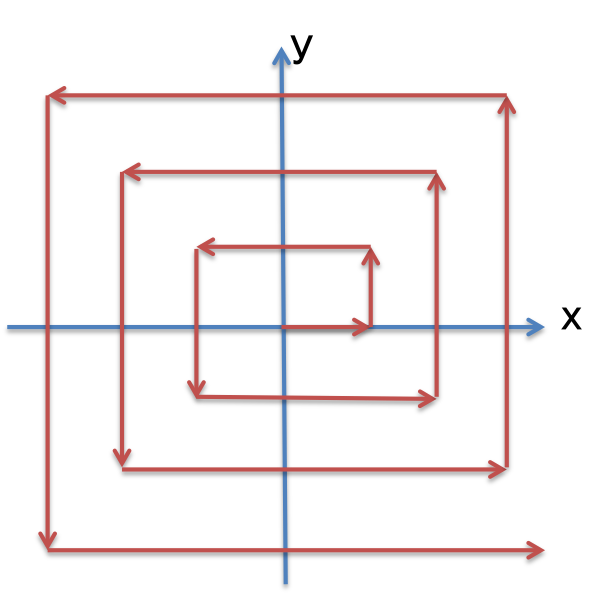
\includegraphics[clip,width=7.0cm]{fig1.png}
    \caption{}
    \label{fig:chokuseki}
  \end{center}
\end{figure}

\item
4と同様に、直積を順番に考え、今度は$(x,y)$の代わりに$\frac{x}{y}$として並べる。つまり\\
\[\frac{0}{0},\frac{1}{0},\frac{1}{1},\frac{0}{1},\frac{-1}{1},\frac{-1}{0},\frac{-1}{-1},\frac{0}{-1},
\frac{1}{-1},\frac{2}{-1},\frac{2}{0},\frac{2}{1},\frac{2}{2},\frac{1}{2},\frac{0}{2},\frac{-1}{2},\frac{-2}{2},\frac{-2}{1},\frac{-2}{0},\frac{-2}{-1},\frac{-2}{-2},\frac{-1}{-2},\frac{0}{-2},\dots\]
ここで、
\begin{enumerate}
\item 分母が0になっているものを削除。
\item 約分すると同じ値になるものは、後に出現しているものを削除。
\end{enumerate}
という操作をして、並べ直すと、
\[\frac{1}{1},\frac{0}{1},\frac{-1}{1},\frac{2}{-1},\frac{2}{1},\frac{1}{2},\frac{-1}{2},\dots\]
ここで、それぞれの分数の現れる順番と分数の値の関係は、自然数の集合から有理数全体の集合への全単射の写像になっている。よって、有理数全体の集合$\mathbb{Q}$は可算集合。
\item
ある集合$A$が可算集合とする。このとき、$A$の無限部分集合$X(X\subset A)$について考える。$A$は可算集合なので、自然数から$A$への全単射の写像$f:\mathbb{N}\to A$が存在する。ここで、$A$の集合を以下のように並べる。
\[f(1),f(2),f(3),f(4),\dots\]
さらに、この順番を保ちながら、$X$に含まれていない要素を取り除き、順番に番号を振る。この番号とそれぞれの要素の対応は、自然数の集合から$X$への全単射になっている。
\end{enumerate}

%%% 7.5
\subsection{}
$f:A\to\mathfrak{P}(A)$が全射とする。
\begin{equation}
X=\{b\in A|b\notin f(b)\} \tag{7.5.1}\\
\end{equation}
とすると、$X\in\mathfrak{P}(A)$かつ$f$が全射なので、$f(x)=X$となる$x\in A$が存在する。\\
もし、$x\in X$と仮定すると、$x$は$(7.5.1)$の条件を満たすはずなので、$x\notin X$となり、矛盾。\\
もし、$x\notin X$と仮定すると、$x$は$(7.5.1)$の条件を満たさないはずなので、$x\in f(x)$となり、矛盾。\\
いずれにしても矛盾するので、$f$は全射ではないことが示された。


%%%% 7.6
\subsection{}
$\mathfrak{P}(\mathbb{N})$を次のような三つの部分集合族$P_1, P_2, P_3$に分割する。$\mathbb{N}$の有限部分集合の全体を$P_1$、$\mathbb{N}$の部分集合で補集合が有限集合であるものの全体を$P_2$、それ以外の$\mathbb{N}$の部分集合の全体を$P_3$とする。$P_1,P_2およびP_1 \cup P_2$は加算集合である。実際、$f_1:\mathbb{N}\to P_1$を以下のように定義する。
\begin{align*}
f_1(1)&=\emptyset\\
f_1(2)&=\{1\}\\
f_1(3)&=\{2\}\\
f_1(4)&=\{1,2\}\\
f_1(5)&=\{3\}\\
f_1(6)&=\{1,3\}\\
f_1(7)&=\{2,3\}\\
f_1(8)&=\{1,2,3\}\\
f_1(9)&=\{4\}\\
\dots
\end{align*}
このとき、$f_1$は全単射になる。\\
また、$f_2:\mathbb{N}\to P_2$を$f_2(n)=\mathbb{N}-f_1(n)$と定義すれば、これは全単射になる。\\
さらに$g:\mathbb{N}\to P_1 \cup P_2$を
\[g(n)=
\begin{cases}
f_1(\frac{n}{2})  \qquad(nが偶数)\\
f_2(\frac{n+1}{2})  \quad(nが奇数)
\end{cases}
\]
と定義すれば、これは全単射になる。\\
$P_1\cup P_2 \sim \mathbb{N}$かつ、$P_2\sim \mathbb{N}$なので、$P_1\cup P_2\sim P_2$。$\mathfrak{P}(\mathbb{N})=P_1\cup P_2 \cup P_3$なので、結局、$\mathfrak{P}(\mathbb{N})\sim P_2 \cup P_3$。\\
また、$I=(0,1]$とすると、$\mathbb{R}\sim I$であることが6章の議論でわかるので、以下では、$P_2\cup P_3 \sim I$を証明する。\\

今、$x\in(0,1]$を$x=0.11010100\dots$のように2進数で表示することにする。ただし、$x=0.1$は$x=0.0\dot{1}$のように、必ず無限小数で表すことにする\footnote{任意の$x\in(0,1]$が、この無限小数の形式で一意に表現できることは、証明すべきことだと思う。ここでは省略する。}。\\
$h:(0,1]\to P_2\cup P_3$を以下のように定義する。\\
\[h(x)=\{n\in\mathbb{N}|xを2進数表示したときの小数第n位が1となる\}\]
$h$は全単射となるので、$P_2\cup P_3 \sim I$が示された\footnote{$h(x)$が無限集合なので、$P_1\cup P_2\cup P_3$でなく、$ P_2\cup P_3$を考える必要があった。}。結局、$\mathfrak{P}(\mathbb{N})\sim\mathbb{R}$が示された。

%%% 7.7
\subsection{}
\begin{enumerate}
\item
\[f:\mathbb{Z}\times(0,1]\to\mathbb{R}\]を\[f(x,y)=x+y\]と定義すれば、$f$は全単射である。よって、$\mathbb{N}\times\mathbb{R}\sim\mathbb{Z}\times(0,1]\sim\mathbb{R}$。

\item
$\frak{P}(A)\sim F(A,\{0,1\})$である。実際、任意の$X\in\frak{P}(A)$に対して、
\[f_X(x)=
\begin{cases}
1 \quad(x\in X)\\
0 \quad(x\notin X)
\end{cases}
\]
と定義される$f_X\in F(A,\{0,1\})$を対応させればこれは全単射になる。よって、$\frak{P}(A)\sim F(A,\{0,1\})$がわかる。\\
また、問7.2により、$F(A\times B,C)\sim F(A,F(B,C))$である。以上より、
\begin{align*}
F(\mathbb{R},\mathbb{R})&\sim F(\mathbb{R},\frak{P}(\mathbb{N}))\\
&\sim F(\mathbb{R},F(\mathbb{N},\{0,1\}))\\
&\sim F(\mathbb{R}\times\mathbb{N},\{0,1\})\\
&\sim F(\mathbb{R},\{0,1\})\\
&\sim \frak{P}(\mathbb{R})
\end{align*}
\end{enumerate}

%%%7.8
\subsection{}
実数値連続関数$f_1,f_2$が任意の$x\in\mathbb{Q}$で$f_1(x)=f_2(x)$ならば、$f_1$と$f_2$は同一である。よって、実数値連続関数全体の集合と$F(\mathbb{Q},\mathbb{R})$は濃度が等しい。\\
問7.4より、$\mathbb{Q}\sim\mathbb{N}$かつ$\mathbb{N}\times\mathbb{N}\sim\mathbb{N}$なので、$\mathbb{Q}\times\mathbb{N}\sim\mathbb{N}$である。
\begin{align*}
F(\mathbb{Q},\mathbb{R})&\sim F(\mathbb{Q}, \frak{P}(\mathbb{N}))\\
&\sim F(\mathbb{Q},F(\mathbb{N},\{0,1\}))\\
&\sim F(\mathbb{Q}\times\mathbb{N}, \{0,1\})\\
&\sim F(\mathbb{N},\{0,1\})\\
&\sim \frak{P}(\mathbb{N})\\
&\sim \mathbb{R}
\end{align*}

%%% 7.9
\subsection{}
整数係数の多項式\[f(x)=a_0+a_1x+a_2x^2+\dots+a_nx^n\quad(n\geq 1, a_n\neq0)\]に対して、\[H(f)=n+|a_0|+|a_1|+\dots+|a_n|\]とおく。$H(f)$は2以上の自然数である。今、自然数$h\geq2$に対して、整数係数の多項式の集合$F_h$を
\[F_h=\{f|H(f)=h\}\]
と定義する。$F_h$は有限集合である。また、n次多項式の根は高々n個なので、$F_h$に属する多項式の根となるような複素数の集合も有限集合である。つまり、$h\geq 2$に対して、$F_h$に属する多項式の根を一列に並べることができる\footnote{たとえば、複素数の実部で昇順に並べて、そのあと虚部で昇順に並べるなどの方法が考えられる}。以上の議論より、任意の代数的数に対して、自然数$n\in\mathbb{N}$を対応させる全単射の写像を作ることができることがわかる。よって、代数的数全体の集合は可算集合である。


%%%7.10
\subsection{}
$z$を整数係数の多項式$f(x)$の根とする。よって、
\[f(z)=0\]
$p$を自然数とすれば\[f(px)=a_0+a_1px+a_2p^2x^2+\dots+a_np^nx^n\]は整数係数の多項式になり、$\frac{z}{p}$は$f(px)$の根である。
したがって、$\alpha$をある超越数とすれば、全ての自然数$p$に対して$p\alpha$も超越数であることがわかる\footnote{$p\alpha$が超越数でない、つまり代数的数であると仮定すると、$\alpha$も代数的数であることになってしまい矛盾。}。代数的数であるような実数の全体は可算集合であり、実数全体の集合$\mathbb{R}$は非可算であるから、超越数の存在がわかる。その一つを$\alpha$とする。$\mathbb{R}$を次のような三つの部分集合$A_1,A_2,A_3$に分割する。代数的数であるような実数の全体を$A_1$とする。\[A_2=\{p\alpha|p\in \mathbb{N}\}\]とする。$A_1,A_2$に属さない実数の全体を$A_3$とする。\\
$A_2\cup A_3$は超越数全体の集合である。$A_1$は問7.9で証明したように加算集合である。
\[g_1(n)=\alpha n\]
という関数$g_1:\mathbb{N}\to A_2$が全単射になるので、$A_2$は加算集合である。$g_2:\mathbb{N}\to A_1$を全単射の写像とすると、
\[h(n)=
\begin{cases}
g_1(\frac{n+1}{2})\quad(nが奇数)\\
g_2(\frac{n}{2})\qquad(nが偶数)\\
\end{cases}
\]
という写像$h:\mathbb{N}\to A_1\cup A_2$が全単射になるので、$A_1\cup A_2$も可算集合である。特に、$A_1\cup A_2\sim A_2$となる。よって、$\mathbb{R}=A_1\cup A_2\cup A_3\sim A_2\cup A_3$。

%%% section 8
\section{二項関係}

%%% 8.1
\subsection{}
\begin{enumerate}
\item $G(\rho_1)=\{(x,y)|x\geq0,y\geq0\}$について
\begin{enumerate}
\item 反射律 満たさない\\
$x=-1$のとき、$x\rho_1 x$を満たさない。
\item 対称律 満たす\\
$x\geq0,y\geq0$ならば、$y\geq0,x\geq0$である。
\item 推移律 満たす\\
$x\geq0,y\geq0$かつ$y\geq0,z\geq0$ならば$x\geq0,z\geq0$である。
\item 反対称律 満たさない\\
$x=1,y=2$のとき、$x\geq 0,y\geq0$かつ$y\geq0,x\geq0$だが、$x\neq y$。
\end{enumerate}

\item $G(\rho_2)=\{(x,y)|x\leq y\}$について
\begin{enumerate}
\item 反射律 満たす\\
$x\leq x$である。
\item 対称律 満たさない\\
$x=1,y=2$のとき、$x\leq y$だが、$y\leq x$でない。
\item 推移律 満たす\\
$x\leq y$かつ$y\leq z$ならば、$x\leq z$。
\item 反対称律 満たす\\
$x\leq y$かつ$y\leq x$ならば$x=y$である。
\end{enumerate}

\item $G(\rho_3)=\{(x,y)|(x-y)(x+y-1)=0\}$について\\
$f(x,y)=(x-y)(x+y-1)$とおく。
\begin{enumerate}
\item 反射律 満たす\\
$x-x=0$なので$f(x,x)=0$である。
\item 対称律 満たす\\
$f(x,y)=0$のとき、$f(y,x)=(y-x)(y+x-1)=-f(x,y)=0$。
\item 推移律 満たす\\
$f(x,y)=0$と$f(y,z)=0$を仮定する。
\begin{enumerate}
\item $x-y=0,y-z=0$のとき\\
$x-z=0$となるので、$f(x,z)=0$。
\item $x-y=0, y+z-1=0$のとき\\
$x+z-1=0$となるので、$f(x,z)=0$。
\item $x+y-1=0, y-z=0$のとき\\
$x+z-1=0$とのあるので、$f(x,z)=0$。
\item $x+y-1=0, y+z-1=0$のとき\\
$x-z=0$となるので、$f(x,z)=0$。
\end{enumerate}
\item 反対称律 満たさない\\
$x=0.7,y=0.3$のとき、$f(x,y)=0$かつ$f(y,x)=0$だが、$x\neq y$。
\end{enumerate}

\item $G(\rho_4)=\{(x,y)|(x-y)(x-y+1)(x-y-1)=0\}$について\\
$g(x,y)=(x-y)(x-y+1)(x-y-1)$とおく。
\begin{enumerate}
\item 反射律 満たす\\
$x-x=0$なので$g(x,x)=0$。
\item 対称律 満たす\\
$g(x,y)=0$のとき、$g(y,x)=(y-x)\{(y-x)^2-1\}=-g(x,y)=0$。
\item 推移律 満たさない\\
$x=2,y=1,z=0$のとき、$g(x,y)=0$かつ$g(y,z)=0$だが、$g(x,z)\neq 0$。
\item 反対称律 満たさない\\
$x=2,y=1$のとき、$g(x,y)=0$かつ$g(y,x)=0$だが、$x\neq y$。
\end{enumerate}
\end{enumerate}

\subsection{}
定義より、$A\rho B\Longleftrightarrow (A-B)\cup(B-A)が有限集合$。
\begin{enumerate}
\item 反射律\\
$A-A=\emptyset$なので、$A\rho A$。
\item 対称律\\
$(A-B)\cup(B-A)=(B-A)\cup(A-B)$なので、$A\rho B$ならば$B\rho A$。
\item 推移律\\
$(A-B)\cup(B-A)=X,(B-C)\cup(C-B)=Y$が有限集合とする。
\begin{align*}
(A-C)\cup(C-A)&=\{x|(x\in A かつ x\notin C)または(x\in Cかつx\notin A)\}\\
&=\{x|(x\in A かつ x\in B かつ x\notin C)または(x\in A かつ x\notin Bかつx\notin C)または\\
&\qquad\qquad(x\in Cかつx\in Bかつx\notin A)または(x\in Cかつx\notin Bかつx\notin A)\}\\
&\subset\{x|(x\in B かつ x\notin C)または(x\in A かつ x\notin B)または\\
&\qquad\qquad(x\in Bかつx\notin A)または(x\in Cかつx\notin B)\}\\
&=\{x|x\in X またはx\in Y\}\\
&=X\cup Y
\end{align*}
よって、$(A-C)\cup(C-A)$も有限集合
\end{enumerate}


%%%8.3
\subsection{}
\begin{enumerate}
\item 反射律
\[\forall x\in X[f(x)=f(x)]\]
\item 対称律
\[\forall x,y\in X[f(x)=f(y)\Longrightarrow f(y)=f(x)]\]
\item 推移律
\[\forall x,y,z\in X[f(x)=f(y) かつf(y)=f(z)\Longrightarrow f(x)=f(z)]\]
\end{enumerate}
よって、$G(\rho)$は反射律、対称律、推移律を満たす。\\
今、$C(x)=\{a\in X|f(a)=f(x)\}$なので、$\forall a\in C(x)[f(a)=f(x)]$。よって、$g(C(x))=f(x)$とすれば、関数$g:X/\rho\to Y_1$が一意に定義できる。\\
$g$は全射である。実際、$f(X)=\{f(x)\in Y|x\in X\}=Y_1$だから、任意の$y\in Y_1$に対して、$f(x)=y$となる$x$が存在する。よって、任意の$y\in Y_1$に対して、$g(C(x))=y$となる$C(x)\neq\emptyset$が存在する。\\
$g$は単射である。実際、$g(A)=g(B)=f(x)$とすると、$x\in Aかつx\in B$となる。$A$と$B$が交わっているので、$A=B$。

%%%8.4
\subsection{}
図\ref{fig:8.4.1}、図\ref{fig:8.4.2}、図\ref{fig:8.4.3}、図\ref{fig:8.4.4}がそれぞれ答え。
\begin{figure}[htbp]
  \begin{center}
    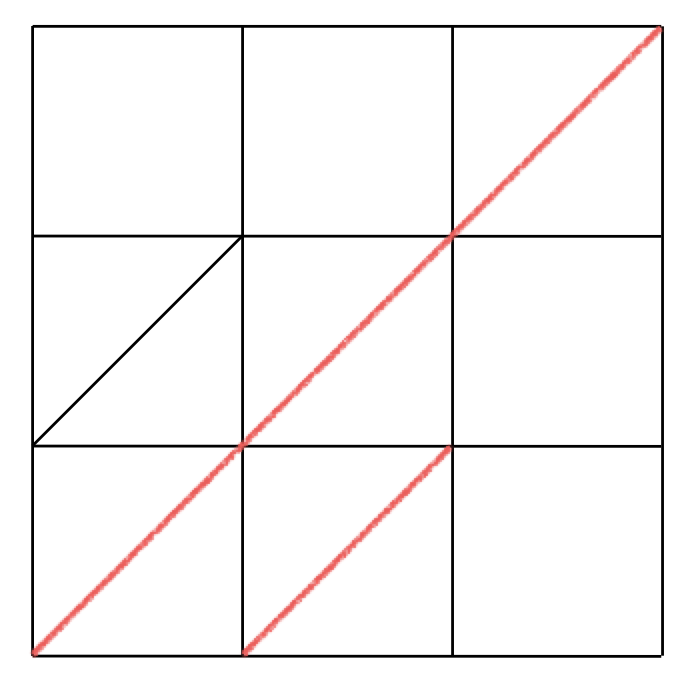
\includegraphics[clip,width=4.0cm]{8_4/8_4_1.png}
    \caption{反射律と対称律を満足するもの}
    \label{fig:8.4.1}
  \end{center}
\end{figure}

\begin{figure}[htbp]
  \begin{center}
    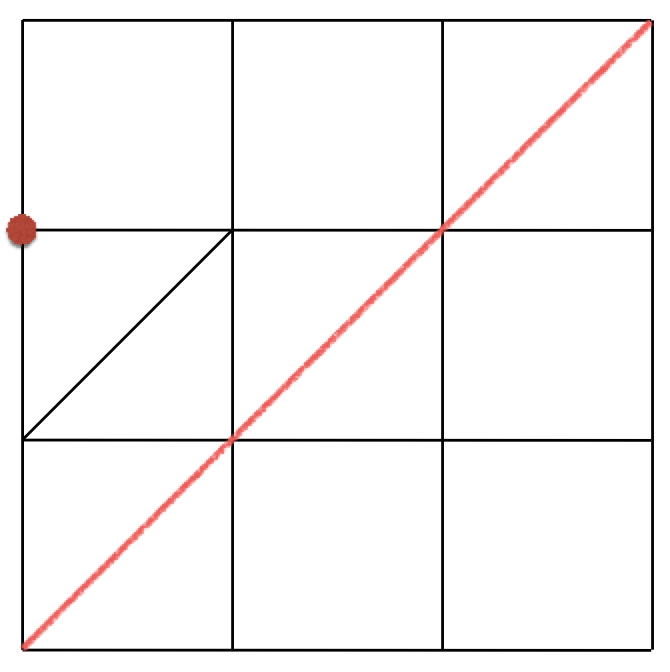
\includegraphics[clip,width=4.0cm]{8_4/8_4_2.png}
    \caption{反射律と推移律を満足するもの}
    \label{fig:8.4.2}
  \end{center}
\end{figure}
\begin{figure}[htbp]
  \begin{center}
    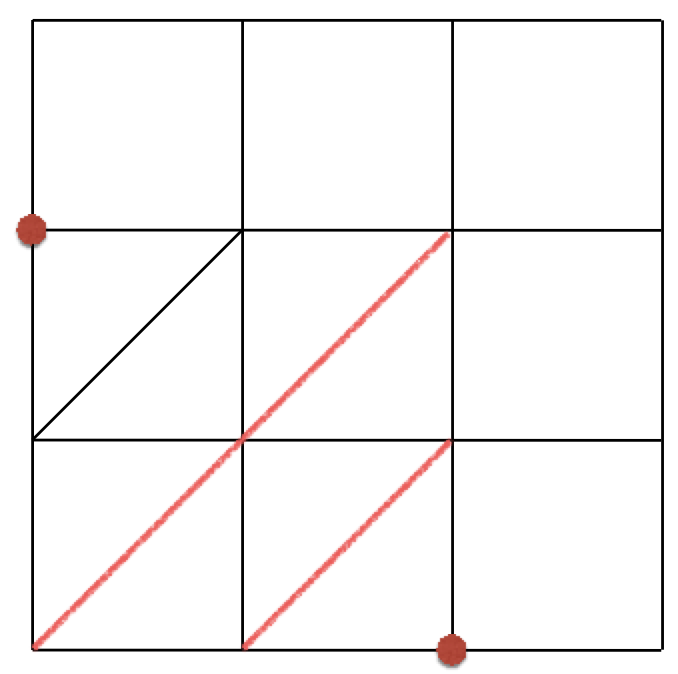
\includegraphics[clip,width=4.0cm]{8_4/8_4_3.png}
    \caption{対称律と推移律を満足するもの}
    \label{fig:8.4.3}
  \end{center}
\end{figure}\begin{figure}[htbp]
  \begin{center}
    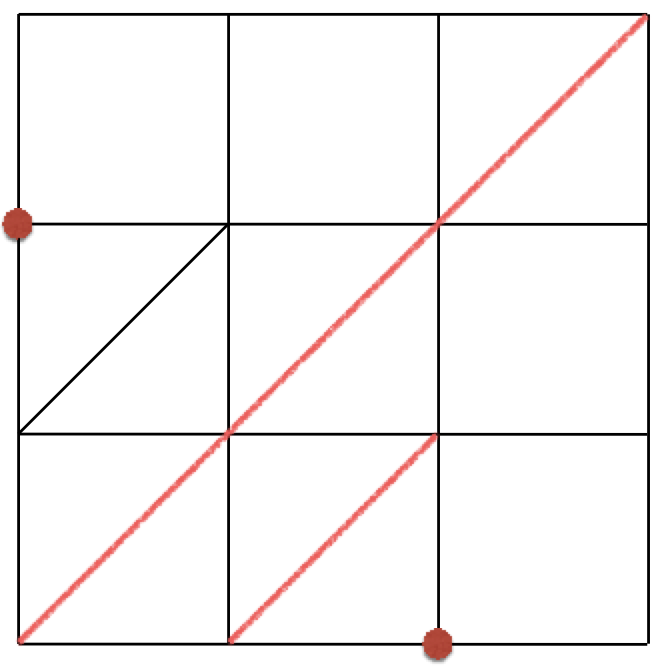
\includegraphics[clip,width=4.0cm]{8_4/8_4_4.png}
    \caption{同値関係であるもの}
    \label{fig:8.4.4}
  \end{center}
\end{figure}

\newpage

%%%8.5
\subsection{}
$\mathfrak{P}(A)$の任意の部分集合$\mathfrak{U}$に対して、
\[\inf \mathfrak{U}=\bigcap(E|E\in\mathfrak{U})\]
\[\sup \mathfrak{U}=\bigcup(E|E\in\mathfrak{U})\]
と定義すれば、確かに
\[\forall B\in \mathfrak{U}[\inf \mathfrak{U}\subset B]\]
\[\forall B\in \mathfrak{U}[B\subset \sup \mathfrak{U}]\]
が成り立つ。

%%% 8.6
\subsection{}
5元束と6元束については、巻末の解答を参照。7元束は図\ref{fig:8_6}のように53種類考えられる\footnote{点の色に特別に意味はない。場合分けの際にわかりやすくするために色付けした。}。
\begin{figure}[htbp]
  \begin{center}
    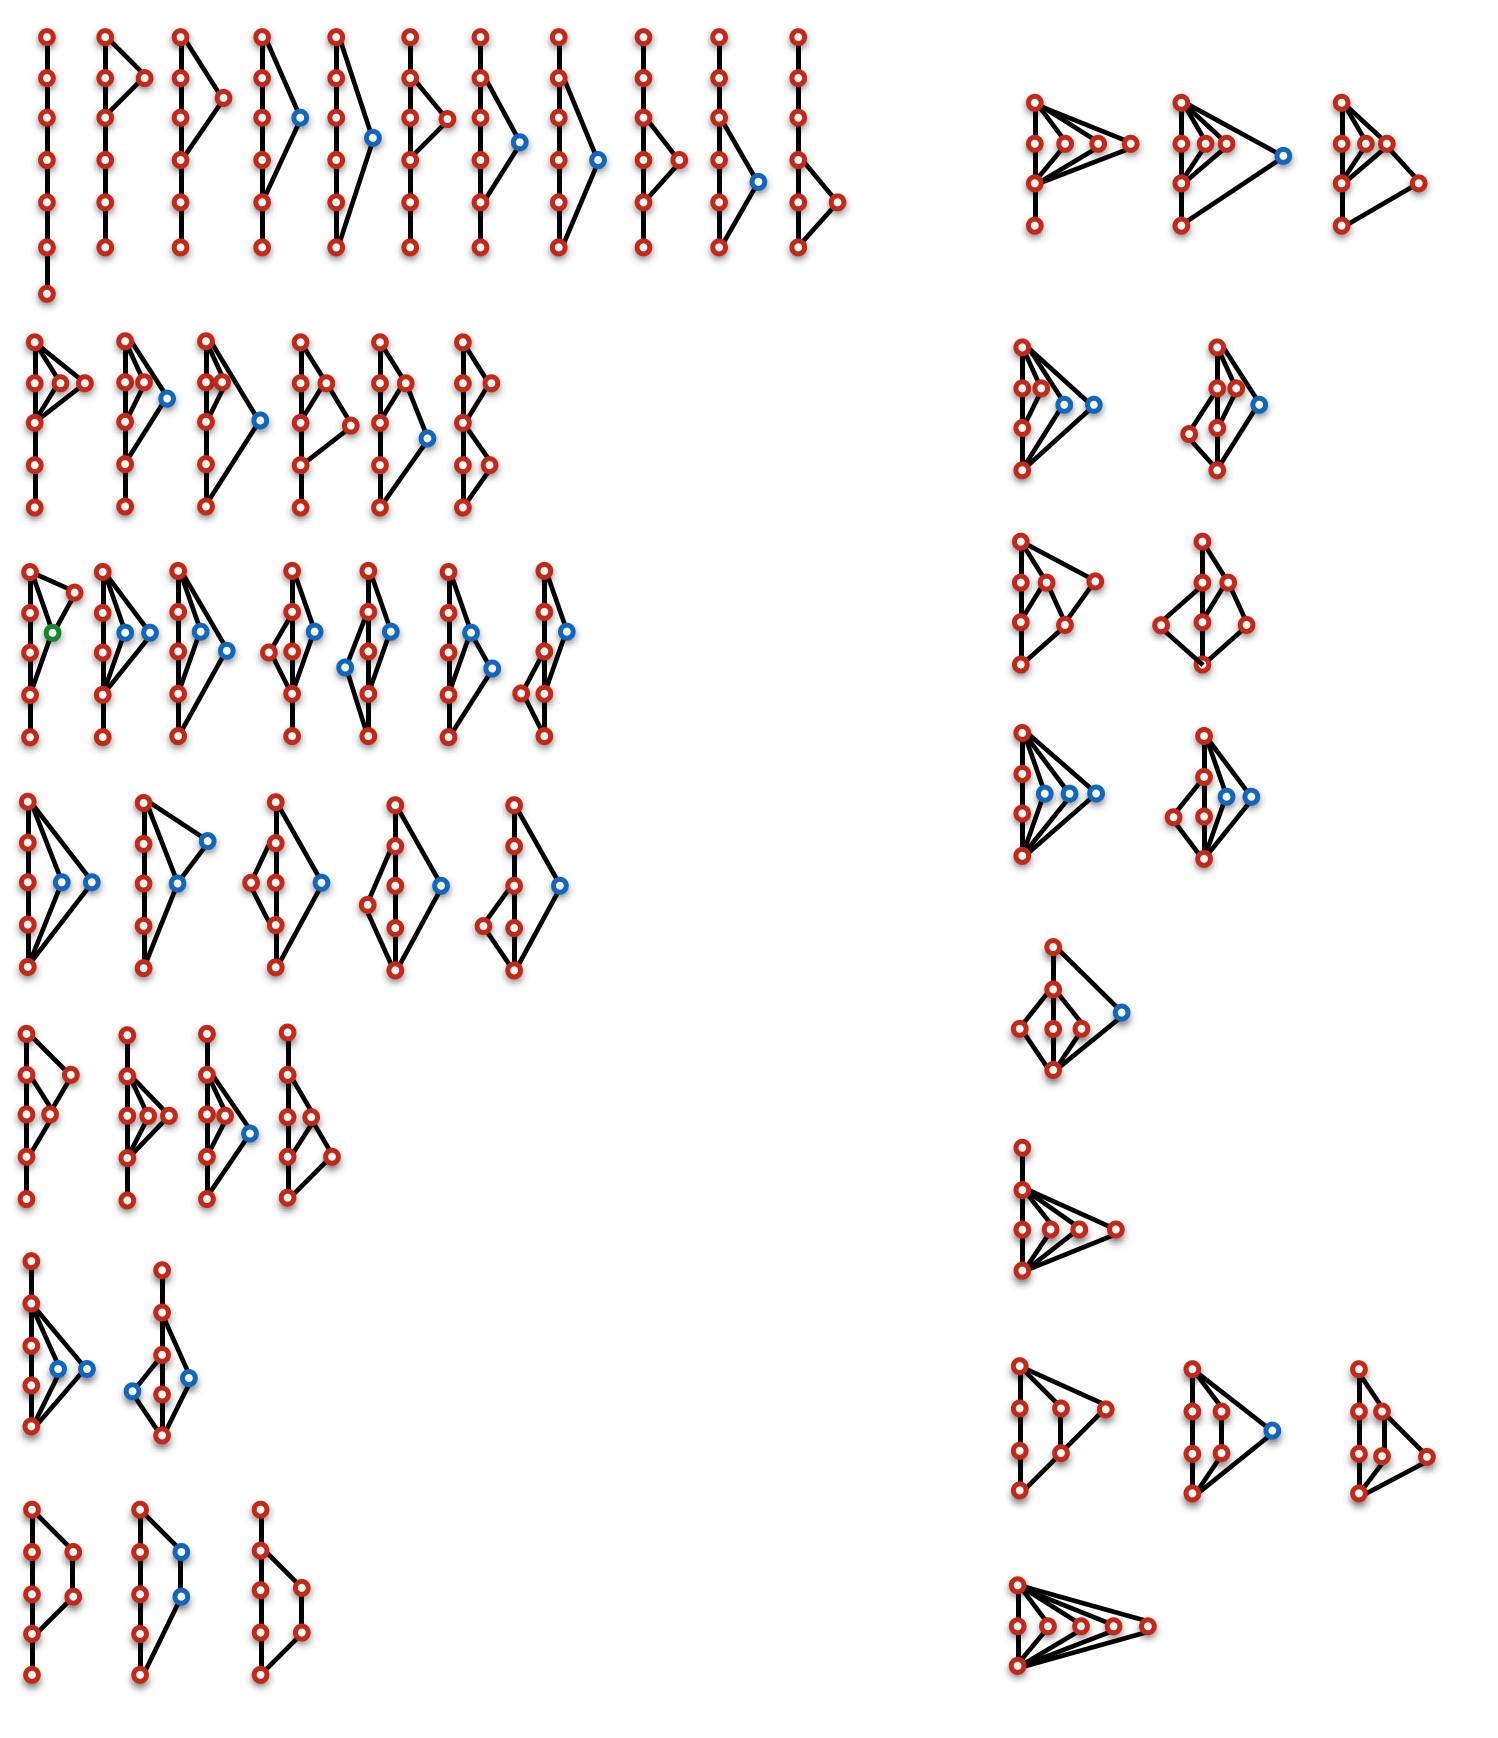
\includegraphics[clip,width=13.0cm]{8_6.png}
    \caption{7元束}
    \label{fig:8_6}
  \end{center}
\end{figure}

\newpage
%%%8.7
\subsection{}
$\mathfrak{U}=\{A\in X|A\subset\varphi(A)\}$とする。$\emptyset\subset\varphi(\emptyset)$なので、$\mathfrak{U}$は空集合にはならない。$E_0=\bigcup (A|A\in\mathfrak{U})$とおけば、$\forall A\in\mathfrak{U}[A\subset\varphi(A)\subset\varphi(E_0)]$なので、$E_0\subset\varphi(E_0)$である。$E_0\subsetneq\varphi(E_0)$とすると、$\varphi(E_0)\in\mathfrak{U}$であることに矛盾。よって、$E_0=\varphi(E_0)$である。


%%% section9
\part{整列集合と選択公理}
\section{整列集合}

%%%9.1
\subsection{}
\begin{align*}
(X\langle a\rangle)\langle b\rangle&=\{x\in X\langle a\rangle|x<b\}\\
&=\{x\in X| x\in X\langle a\rangle かつ x<b\}\\
&=\{x\in X| x<aかつx<b\}\\
&=\{x\in X|x<b\}\\
&=X\langle b\rangle
\end{align*}
ここで、$b<a$という前提により、「$x<aかつx<b\Longleftrightarrow x<b$」という関係を用いた。実際、$x<b$であって、$a\leq x$と仮定すると、$a\leq b$となり矛盾してしまう。

\subsection{}
\subsubsection{整列集合は、そのいかなる切片とも順序同型にならない}
\label{9_2}
ある切片$a\in X$に対して、$(X,\leq)\simeq(X\langle a\rangle,\leq)$が成り立つと仮定すると、順序を保つ全単射$f:X\to X\langle a\rangle$が存在することになる。$f$は単射なので、定理9.1により
\[\forall x\in X[x\leq f(x)]\]
が成り立つはずである。しかし、$f(a)\in X\langle a\rangle$なので、$f(a)<a$となってしまい矛盾。結局、$(X,\leq)\simeq(X\langle a\rangle,\leq)$ではないことがわかる。
\subsubsection{整列集合の相異なる二つの切片は互いに順序同型にならない}
整列集合の部分集合は整列集合である。今、$Y$を整列集合とし、$a,b (a<b, a\in Y, b\in Y)$に対して、
\[X= Y\langle b\rangle\]
とおくと、
\begin{align*}
X\langle a\rangle&=\{x\in X|x<a\}\\
&=\{x\in Y\langle b\rangle| x<a\}\\
&=\{x\in Y| x<aかつx<b\}\\
&=\{x\in Y|x<a\}\\
&=Y\langle a\rangle
\end{align*}
となり、$X\langle a\rangle=Y\langle a\rangle$が成り立つ。すると、\ref{9_2}と同様に、$(Y\langle a\rangle,\leq)\simeq(Y\langle b\rangle,\leq)$にはならないことが証明できる。

\subsection{}
$(A,\leq)$および$(B,\leq)$を整列集合とし、$f:A\to B$を順序同型写像とする。今、$f$は全単射なので、
\[x<y\Longleftrightarrow f(x)<f(y)\]
が成り立つ\footnote{左から右へは、$f$が順序を保ちかつ単射であることから証明できる。右から左へは、$f$が全射であることと、逆写像$f^{-1}$が存在することから証明できる。}。よって、任意の$a\in A$に対して、
\begin{align*}
f(A\langle a\rangle)&=\{f(x)\in B| x\in A\langle a\rangle\}\\
&=\{f(x)\in B|x<a かつ x\in A\}\\
&=\{f(x)\in B|f(x)<f(a) かつ x\in A\}\\
&=\{y\in B|y<f(a)\}\\
&=B\langle f(a)\rangle
\end{align*}

%%%% 9.4
\subsection{}
以下では、$\varphi:X_1\to Y_1$が順序同型写像であることを証明するため、$\varphi$が全単射の写像であることと、$\varphi$が順序を保つ写像であることを証明する。定義より、$X_1,Y_1$はそれぞれ、
\[X_1=\{a\in X|\exists b\in Y[X\langle a\rangle\simeq Y\langle b\rangle]\}\]
\[Y_1=\{b\in Y|\exists a\in X[X\langle a\rangle\simeq Y\langle b\rangle]\}\]
このとき、各元$a\in X_1$に対して、$X\langle a\rangle\simeq Y\langle b\rangle$となる$b\in Y_1$がただ一つ存在する。実際、$b_1,b_2\in Y_1$が$X\langle a\rangle\simeq Y\langle b_1\rangle$かつ$X\langle a\rangle\simeq Y\langle b_2\rangle$となると仮定すると、$Y\langle b_1\rangle\simeq Y\langle b_2\rangle$であり、順序同型写像$f:Y\langle b_1\rangle\to Y\langle b_2\rangle$が存在する。$b_1<b_2$と仮定すると、順序を保つ単射$f$に対して、$f(b_1)<b_2$となり、定理9.1に矛盾する。$b_1>b_2$としてもやはり矛盾が生じるので、$b_1=b_2$になるはずである。結局、$X\langle a\rangle\simeq Y\langle b\rangle$となる$b$がただ一つ存在することがわかった。さて、以上の議論を逆に$b$を中心に展開すると、任意の$b\in Y_1$に対して、$X\langle a\rangle\simeq Y\langle b\rangle$となる$a$がただ一つ存在することになる。よって、$b=\varphi(a)$と定義される写像$\varphi$は全単射である。\\
 $a_1,a_2\in X_1$が$a_1\leq a_2$であると仮定する。$X\langle a_1\rangle\simeq Y\langle \varphi(a_1)\rangle$の順序同型写像$\psi_1$
\[\psi_1:Y\langle \varphi(a_1)\rangle\to X\langle a_1\rangle\]
は順序を保つ全単射の写像である。また、$X\langle a_2\rangle\simeq Y\langle \varphi(a_2)\rangle$の順序同型写像$\psi_2$
\[\psi_2:X\langle a_2\rangle\to Y\langle \varphi(a_2)\rangle\]
も順序を保つ全単射の写像である。よって、$\psi=\psi_2\circ\psi_1$
\[\psi:Y\langle \varphi(a_1)\rangle\to Y\langle \varphi(a_2)\rangle\]
は順序を保つ単射の写像である\footnote{$X\langle a_1\rangle\subset X\langle a_2\rangle$なので$\psi$は全射とは限らない。}ので、定理9.1より、$\varphi(a_1)\leq\varphi(a_2)$である\footnote{$\varphi(a_1)>\varphi(a_2)$と仮定すると、$\psi(\varphi(a_2))<\varphi(a_2)$となり、定理9.1に反する}。結局\[a_1\leq a_2\Longleftrightarrow\varphi(a_1)\leq\varphi(a_2)\]となり、$\varphi$が順序を保つ写像であることが証明できた。\\
 以上より、$\varphi:X_1\to Y_1$は順序同型写像である。

\subsection{}
(1)と(2)が同時に成り立つと仮定し、順序同型$X\simeq Y, X\simeq Y\langle b\rangle$が成り立つとする。すると、$Y\simeq Y\langle b\rangle$が成り立つ。$Y\simeq Y\langle b\rangle$の順序同型写像を$f:Y\to Y\langle b\rangle$とすると、$f(b)<b$となり、定理9.1に矛盾する。従って、(1)と(2)は同時には成り立たない。\\
 (1)と(3)が同時に成り立たないことも同様に証明できる。

\section{選択公理}
\subsection{}
$f$を集合$A$の上の一つの選択関数とする。$f$は$A$の空でない部分集合の全体$\mathfrak{U}=\mathfrak{P}(A)-\{\emptyset\}$から、$A$への写像であり、$f(B)\in B\subset A$である。$m<n$と仮定すると
\[a_n=f(A-\{a_1,\dots,a_m,\dots,a_{n-1}\})\]
となり、$a_m\notin A-\{a_1,\dots,a_m,\dots,a_{n-1}\}$なので、$a_m\neq a_n$。$n<m$の場合も同様に証明できる。

\subsection{}	
$W_\infty$の一つの上界が$W_\infty$に含まれるならば、それは$W_\infty$の最大限になる。以下では、$w\in W_\infty$であることを背理法で証明する。\\
 $w\notin W_\infty$と仮定し、
\[\Delta_\infty=\{x\in X| a\in W_\infty ならば a<x\}\]
とおく。$w\notin W_\infty$であり、$w$が$W_\infty$の上界であることから$w\in \Delta_\infty$。よって$\Delta_\infty\neq\emptyset$である。そこで、$z=f(\Delta_\infty)$とおく。このとき、$W_*=W_\infty\cup\{z\}$は整列集合である。
$W_\infty=W_*\langle z\rangle$であるから、$\Delta_\infty=\Delta(W_*,z)$であり、$W_*$も$f$-列になる\footnote{
\begin{enumerate}
\item
$a\in W_\infty$のとき、
\begin{align*}
\Delta(W_*, a)&=\{x\in X|b\in W_*\langle a\rangle ならば b<x\}\\
&=\{x\in X|b\in W_\infty\langle a\rangle ならば b<x\}\\
&=\Delta(W_\infty, a)
\end{align*}
なので、$f(\Delta(W_*, a))=f(\Delta(W_\infty, a))=f(a)$である。
\item
$a=z$のとき、
\begin{align*}
\Delta(W_*, z)&=\{x\in X|b\in W_*\langle z\rangle ならば b<x\}\\
&=\{x\in X|b\in W_\infty ならば b<x\}\\
&=\Delta_\infty
\end{align*}
なので、$f(\Delta(W_*, z))=f(\Delta_\infty)=z$である。
\end{enumerate}
}。

これは$W_\infty$が最大$f$-列であることに矛盾する。したがって、$w\in W_\infty$であることがわかった。よって、$w$は$W_\infty$の最大限である。


%%%%%  section 11  %%%%%%%%%%%
\section{整列可能定理}
\subsection{}
\subsubsection{}
\label{11_1_1}
$W=\bigcup(W_\lambda|\lambda\in\Lambda)$の2元$x,y$に対して、
\[x\in W_\lambda,\quad y\in W_\lambda\]
となる元$\lambda\in\Lambda$が存在しないと仮定する。すると、ある$\lambda_1,\lambda_2\in\Lambda$に対して
\[\lambda_1\neq\lambda_2\]
\[x\in W_{\lambda_1},\quad x\notin W_{\lambda_2},\quad y\in W_{\lambda_2},\quad y\notin W_{\lambda_1}\]
が成り立つことになる。これは「$\Lambda$の異なる2元$\alpha,\beta$に対しては、常に$(W_\alpha,\leq_\alpha),(W_\beta,\leq_\beta)$の中のいずれか一方は他方の切片になっている」という仮定に反する。

\subsubsection{}
\label{11_1_2}
「$\Lambda$の異なる2元$\alpha,\beta$に対しては、常に$(W_\alpha,\leq_\alpha),(W_\beta,\leq_\beta)$の中のいずれか一方は他方の切片になっている」という仮定により、ある$\lambda\in\Lambda$に対して、
$x,y\in W_\lambda かつ x\leq_\lambda y$
が成り立つならば、任意の$\lambda'\in\Lambda$に対しても、
\[x,y\in W_{\lambda'}\Longrightarrow x\leq_{\lambda'}y\]
が成り立つ。

\subsubsection{}
$W$の上の二項関係$\leq$は順序関係であることを証明する。
\begin{enumerate}
\item{反射律}\\
$\forall\lambda\in\Lambda[x\in W_\lambda\Longrightarrow x\leq_\lambda x]$なので、$\forall x\in W[x\leq x]$が成り立つ。

\item{推移律}\\
\ref{11_1_1}と同様の議論により、任意の3元$x,y,z\in W$に対して
\[x\in W_\lambda,\quad y\in W_\lambda,\quad z\in W_\lambda\]
となる元$\lambda\in\Lambda$が存在することがわかる。$\leq_\lambda$が順序関係なので、
\[x\leq_\lambda y かつ y\leq_\lambda z ならば x\leq_\lambda z\]
が成り立つ。よって、$\leq$も
\[x\leq y かつ y\leq z ならば x\leq z\]
が成り立つ。

\item{反対称律}\\
\ref{11_1_1}により、任意の2元$x,y\in W$に対して
\[x\in W_\lambda,\quad y\in W_\lambda\]
となる元$\lambda\in\Lambda$が存在する。$\leq_\lambda$が順序関係なので、
\[x\leq_\lambda y かつ y\leq_\lambda x ならば x=y\]
が成り立つ。よって、$\leq$も
\[x\leq y かつ y\leq x ならば x=y\]
が成り立つ。\\
\end{enumerate}
以上より、$W$の上の二項関係$\leq$は順序関係であることがわかった。\\

$W$は整列集合になることを証明する。\\
$W$の空でない部分集合を$U$とする。$U$の元$x$に対して、$x\in W_\lambda$となる$\lambda\in\Lambda$が存在する。$W_\lambda$は整列集合なので、$W_\lambda\cap U$には最小値$y=\min(W_\lambda\cap U)$が存在する。この$y$は$U$の最小値でもある。実際、もしも$z<y$となる$z\in U$が存在すると仮定すると、$z<y$にも関わらず、$z\notin W_\lambda$ かつ $y\in W_\lambda$となってしまう。$z\in W$なので、$z\in W_{\lambda'}$という$\lambda'\in\Lambda$が存在するはずだが、これは「$\Lambda$の異なる2元$\alpha,\beta$に対しては、常に$(W_\alpha,\leq_\alpha),(W_\beta,\leq_\beta)$の中のいずれか一方は他方の切片になっている」という仮定に矛盾する。結局、$y=\min(W_\lambda\cap U)$は$U$の最小値でもある。半順序集合$(W,\leq)$の任意の部分集合$U$に対して最小値が存在するので、$W$は整列集合である。


\subsubsection{}
\ref{11_1_2}により、$\forall\lambda\in\Lambda$に対して、\[x\leq_\lambda y\Longrightarrow x\leq y\]が成り立つ。
また、定義より$\forall \lambda\in\Lambda[W_\lambda\subset W]$が成り立つ。よって、「各$\lambda\in\Lambda$に対して、$(W_\lambda,\leq_\lambda)$は$(W,\leq)$に一致するかまたは$(W,\leq)$の切片になる」ということを証明するためには、
\[\forall x\in W-W_\lambda[\forall y\in W_\lambda[y<x]]\]
が成り立つことを証明すればよい。ある$x\in W-W_\lambda$に対して、$x\leq y$となる$y\in W_\lambda$が存在すると仮定すると、$x\leq y$にも関わらず、$x\notin W_\lambda$かつ$y\in W_\lambda$となってしまい、「$\Lambda$の異なる2元$\alpha,\beta$に対しては、常に$(W_\alpha,\leq_\alpha),(W_\beta,\leq_\beta)$の中のいずれか一方は他方の切片になっている」という仮定に矛盾する。以上より、各$\lambda\in\Lambda$に対して、$(W_\lambda,\leq_\lambda)$は$(W,\leq)$に一致するかまたは$(W,\leq)$の切片になっている。

\subsection{}
\subsubsection{例11.1}
$A$の部分集合$W$と単射の関数$f:W\to B$の組$(W,f)$全体の集合を$\mathfrak{U}$とおく。$\mathfrak{U}$は空ではない。実際、$A$の一つの元$a$だけからなる集合$W=\{a\}$から$B$への写像$f:\{a\}\to B$は単射である。$\mathfrak{U}$の元$(W,f),(W',f')$に対して、$(W,f)\leq (W',f')$を以下のように定義する。
\[ W\subset W' かつ \forall x\in W[f(x)=f'(x)]\]
このとき、$(\mathfrak{U},\leq)$は帰納的半順序集合になる。実際、半順序集合になることは反射律、推移律、反対称律を確かめることでわかる。また、全順序部分集合$\mathfrak{W}$に対して、\[X=\bigcup_{(W,f_W)\in \mathfrak{W}}W\]と$X$を定義する。さらに、$f_X:X\to B$を、$x\in W$となる$(W,f_W)\in\mathfrak{W}$が存在するときに$f_X(x)=f_W(x)$と定義する。$\mathfrak{W}$が全順序集合であることから、$f_X$は一意に定義されている。
このとき、$(X,f_X)$は$\mathfrak{W}$の上界になる。実際、任意の$(W,f_W)\in\mathfrak{W}$に対して、$W\subset X$と、$\forall x\in W[f_W(x)=f_X(x)]$が成り立つので、任意の$(W,f_W)\in\mathfrak{W}$に対して$(W,f_W)\leq (X,f_X)$が成り立つ。結局、$(X,f_X)$は$\mathfrak{W}$の上界である。\\
ツォルンの補題により帰納的半順序集合は極大元を持つので、$(W,f)\in\mathfrak{U}$を一つの極大元とすれば、$W=A$または$f(W)=B$のいずれかが成り立つ。$W=A$のときは$A$から$B$への単射が存在し、$f(W)=B$のときは$B$から$A$への単射が存在する。

\subsubsection{例11.2}
$\mathbb{R}$の部分集合$B$は、$B$に属する有限個の実数が常に$\mathbb{Q}$上一次独立であるとき、$\mathbb{Q}$上一次独立な集合という。$\mathbb{Q}$上一次独立な集合の全体を$\mathfrak{B}$とする。$\mathfrak{B}$は空でない。実際、たとえば$\{1\}$は$\mathbb{Q}$上一次独立な集合である。$X,Y\in\mathfrak{B}$に対して、$X\leq Y$を以下のように定義する。
\[X\leq Y\Longleftrightarrow X\subset Y\]
このとき、$(\mathfrak{B},\leq)$は帰納的半順序集合になる。実際、全順序部分集合$\mathfrak{A}$に対して、
\[U=\bigcup_{X\in\mathfrak{A}}X\]
とおけば、$U\in\mathfrak{B}$であり\footnote{$\mathfrak{A}$は全順序部分集合なので、任意の実数$x_1,x_2,\dots,x_r\in U$に対して、ある$X\in\mathfrak{A}$が存在し、$x_1,x_2,\dots,x_r\in X$となるはずである。$X$は$\mathbb{Q}$上一次独立な集合なので、$x_1,x_2,\dots,x_r$は一次独立であり、$U\in\mathfrak{B}$であることがわかる。}、任意の$X\in\mathfrak{A}$に対して、$X\subset U$、つまり$X\leq U$が成り立ち、$U$は上界になっている。よって、任意の全順序部分集合に対して上界が存在するので、$(\mathfrak{B},\leq)$は帰納的半順序集合になっている。$B$を$\mathfrak{B}$の一つの極大元とする。すなわち$B$は$\mathbb{Q}$上一次独立な極大集合である。このとき、任意の実数は$B$に属する有限個の実数の$\mathbb{Q}$上一次結合になる\footnote{ある実数$x$が$B$に属する有限個の実数の$\mathbb{Q}$上一次結合にならなければ、$B\cup\{X\}$も$\mathbb{Q}$上一次独立な集合のはずである。これは$B$が$\mathbb{Q}$上一次独立な極大集合であることに矛盾してしまう。}。よって、$B$は一つのハメル基である。






%%%%%%%%%%%%%%%%%%%%%%%%%%%%%%%%%%
%%%%%%%%%     PART 4     %%%%%%%%%
%%%%%%%%%%%%%%%%%%%%%%%%%%%%%%%%%%
\part{距離空間}
\section{ユークリッド空間}


%%%%%%%%%%%% 問12.1 %%%%%%%%%%%%
\subsection{}
\subsubsection{$(M^i)^i=M^i$の証明}
定義より$a\in M^i$ とは
\[  \exists \epsilon > 0 [B_n(a;\epsilon )\subset M] \]
のことであり、$a\in(M^i)^i$とは
\[\exists \epsilon > 0 [B_n(a;\epsilon )\subset M^i] \]
のことである。$(M^i)^i\subset M^i$は定義より成り立つ。以下では、$M^i\subset (M^i)^i$を示す。\\
$x\in M^i$と仮定すると、$B_n(x;\epsilon)\subset M$が成り立つような、$\epsilon >0$が存在する。点$y\in B_n(x;\epsilon)$に対して、$\delta = \epsilon-d^{(n)}(x,y)$とおくと、$\delta >0$。今、点$z\in B_n(y;\delta)$について
\begin{eqnarray*}
d^{(n)}(x,z)&\leq&d^{(n)}(x,y)+ d^{(n)}(y,z)\\
 &<& d^{(n)}(x,y)+\delta \\
 &=& \epsilon
\end{eqnarray*}
これより、$z\in B_n(x;\epsilon)$であり、$z\in M$が示せた。\[\exists \delta > 0[B_n(y,\delta)\subset M]\]なので、$y\in M^i$であり、\[\exists\epsilon >0[B_n(x;\epsilon)\subset M^i]\]なので、$x\in (M^i)^i$である。

\subsubsection{$(M^a)^a=M^a$の証明}
$M^a \subset (M^a)^a$は定義から成り立つ。よって、以下では$(M^a)^a\subset M^a$を示す。\\
$x\in (M^a)^a$を仮定すると、任意の$\epsilon > 0$について、
\[B_n(x;\epsilon)\cap M^a \neq \emptyset\]
が成り立つ。これを書き換えて、\[B_n(x;\epsilon)\cap (M^i \cup M^f) \neq \emptyset\]
つまり、\[B_n(x;\epsilon)\cap M^i \neq \emptyset\ \ \ または\ \  B_n(x;\epsilon) \cap M^f \neq \emptyset\]
が成り立つ。以下ではこれら2つの場合で分けて考える。
\begin{enumerate}
\item
 $B_n(x;\epsilon)\cap M^i \neq \emptyset$が成り立つとき\\
 $B_n(x;\epsilon)\cap M \neq \emptyset$が成り立つ。
\item
 $B_n(x;\epsilon) \cap M^f \neq \emptyset$が成り立つとき\\
ある点$y\in(B_n(x;\epsilon)\cap M^f)$が存在する。$y\in M^f$なので、任意の$\delta >0$について,
$B_n(y;\delta)\cap M \neq \emptyset$である。ここで、$\delta=\epsilon-d^{(n)}(x,y)$とおくと、$\delta>0$である。点$z\in B_n(y;\delta)$について
\begin{eqnarray*}
d^{(n)}(x,z) &\leq& d^{(n)}(x,y)+d^{(n)}(y,z)\\
&<& d(x,y)+\delta\\
&=&\epsilon
\end{eqnarray*}
となるので、$B_n(y;\delta)\subset B_n(x;\epsilon)$。よって、$B_n(x;\epsilon)\cap M\neq \emptyset$が示せた。
\end{enumerate}
いずれの場合でも、 $B_n(x;\epsilon)\cap M \neq \emptyset$が成り立つので、$x\in M^a$が成り立つ。



%%%%%%%%% 問 12.2 %%%%%%%%%%%%%
\subsection{}
\subsubsection{}
$M=(a_1,b_1)\times(a_2,b_2)\times ... \times(a_n, b_n)$とおく。また、ある$x=(x_1, ..,x_n)\in M$に対して、
\[l=\min (b_1-x_1 , x_1-a_1, b_2-x_2, x_2-a_2,...,b_n-x_n, x_n-a_n)\]
とおく。このとき、$l>0$である。\\
今、$y=(y_1,...,y_n)\in B_n(x;l)$とする。$d^{(n)}(x,y) < l$だから、各$i=1,2,...,n$について、
\[x_i-(a_i-x_i) \leq x_i-l < y_i < x_i + l \leq x_i + (b_i-x_i) \]
つまり、
\[ a_i < y_i < b_i\]
が成り立つ。以上より、$y\in M$。\\
$\forall x\in M[\exists l > 0 [B_n(x;l)\subset M]]$なので、$M$は開集合である。


\subsubsection{}
$M=[a_1,b_1]\times[a_2,b_2]\times ... \times[a_n, b_n]$とおく。$M=\bar{M}$を示すためには、$\bar{M}\subset M$を示せば十分。そのために、$x\notin M$を仮定して、$x\notin \bar{M}$を導く。\\
$x\notin M$と仮定する。すると少なくとも一つの$i(=1,..,n)$で$x_i<a_i$または$b_i < x_i$が成り立つ。
\begin{enumerate}
\item $x_i < a_i$の場合\\
$y=(y_1,...,y_n)\in B_n(x; a_i-x_i)$とすると、
\[y_i < x_i + (a_i-x_i)= a_i\]
となり、$y\notin M$。よって、$a_i-x_i>0$に対して、$B_n(x;a_i-x_i)\cap M = \emptyset$となるので、$x\notin \bar{M}$
\item $b_i < x_i$の場合\\
$z=(z_1,...,z_n)\in B_n(x; x_i-b_i)$とすると、
\[  x_i - (x_i - b_i) < z_i\]
となり、$b_i < z_i$。よって、$z\notin M$。$x_i-b_i >0$に対して$B_n(x;x_i-b_i)\cap M = \emptyset$となるので、$x\notin \bar{M}$
\end{enumerate}
以上より、$x\notin M$を仮定して、$x\notin \bar{M}$を示せた。よって、$\bar{M} \subset M$。


%%%%%%%%%%% 12.3 %%%%%%%%%%%%5
\subsection{}
\subsubsection{}
$\mathbb{R}^n\in \mathfrak{U}$ である。
実際、
${(\mathbb{R}^n)}^c=\emptyset$なので、${(\mathbb{R}^n)}^f={(\mathbb{R}^n)}^e=\emptyset$である。よって、${(\mathbb{R}^n)}^a=\mathbb{R}^n$。\\
また、$\emptyset\in\mathfrak{U}$である。実際、$\emptyset^i=\emptyset$であり、 $\emptyset^f=\emptyset$である。よって、$\emptyset^a=\emptyset$
\subsubsection{}
$A_1,...,A_k\in \mathfrak{U}$とし、$A=A_1\cup...\cup A_k$とする。\\
$x\in A^a$とすれば、
\[\forall \epsilon >0 [B_n(x;\epsilon)\cap A\neq \emptyset]\]
つまり、
\[\forall \epsilon >0 [B_n(x;\epsilon)\cap (A_1\cup A_2\cup ...\cup A_k)\neq \emptyset]\]
このとき、
\[\forall\epsilon >0[B_n(x;\epsilon)\cap A_j\neq \emptyset]\]
となる$j(1\leq j \leq k)$が存在する。なぜなら、そのような$j$が存在しないとすると、ある$m(1\leq m\leq k)$、$\epsilon_0<\epsilon_1$に対して、
\[B_n(x;\epsilon_0)\cap A_m\neq \emptyset かつ B_n(x;\epsilon_1)\cap A_m = \emptyset\]
となることになってしまい、これは不合理。\\
これより、$x$は$A_j$の触点であり、$A_j\in\mathfrak{U}$だから、$x\in A_j$である。よって、$x\in A$。以上より$A^a\subset A$なので$A\in\mathfrak{U}$。



%%%%%%%%%%%%% 12.4 %%%%%%%%%%
\subsubsection{}
\[\forall\epsilon>0[B_n(x;\epsilon)\cap(\bigcap_{\lambda\in\Lambda}A_\lambda)\neq\emptyset]\]
これを書き換えて、
\[\forall\epsilon>0[\bigcap_{\lambda\in\Lambda}(B_n(x;\epsilon)\cap A_\lambda)\neq\emptyset]\]
これから以下のことが言える$(\Longrightarrow)$
\[\forall\epsilon>0[\forall\lambda\in\Lambda[B_n(x;\epsilon)\cap A_\lambda\neq\emptyset]]\]
よって、
\[\forall\lambda\in\Lambda[\forall\epsilon>0[B_n(x;\epsilon)\cap A_\lambda\neq\emptyset]]\]
任意の$\lambda\in\Lambda$について、$A_\lambda\in\mathfrak{U}$なので、
\[\forall\lambda\in\lambda[x\in A_\lambda]\]
よって、$x\in A$だから、$A^a\subset A$。以上より、$A\in\mathfrak{U}$。

\subsection{}
\subsubsection{}
$M$に包まれる開集合$N$で、$N-M^i\neq \emptyset$となるものが存在すると仮定する。
$x\in N-M^i$とすると$N$は開集合なので、$x$は$N$の内点であり、
\[\exists\epsilon>0[B_n(x;\epsilon)\subset N]\]
となる。$N\subset M$なので、
\[\exists\epsilon>0[B_n(x;\epsilon)\subset M]\]
のはずだが、これは$x$が$M$の内点となることを意味し、$x\notin M^i$に矛盾する。
以上より、$M^i$は$M$に包まれる最大の開集合である。

\subsubsection{}
$M$を包む閉集合$N$で、$\bar{M}-N\neq \emptyset$となるものが存在すると仮定する。
$x\in \bar{M}-N$とすると$N=\bar{N}$なので、$x\notin\bar{N}$つまり、$x$は$N$の外点であり、
\[\exists\epsilon>0[B_n(x;\epsilon)\cap N=\emptyset]\]
である。ここで、$M\subset N$であるので、
\[\exists\epsilon>0[B_n(x;\epsilon)\cap M=\emptyset]\]
$x$は$M$の外点でもあることになってしまい、$x\in \bar{M}$に矛盾する。
以上より、$\bar{M}$は$M$を包む最小の閉集合である。








%%%% Section 13 %%%%%
\section{距離空間}

\subsection{}
\begin{enumerate}
\item[{[$D_1$]}] 
$|f(x)-g(x)|\geq 0$なので、任意の$f,g\in B[a,b]$について、$d(f,g)\geq 0$。
$f=g$ならば、$d(f,g)=\sup\{0\}=0$。逆に、$d(f,g)=\sup\{|f(x)-g(x)|,\ \ a\leq x\leq b\}=0$ならば、$\forall x (a\leq x\leq b)[f(x)=g(x)]$となるので、$f=g$である。

\item[{[$D_2$]}]
任意の$f,g\in B[a,b]$について、
\begin{align*}
d(f,g)&=\sup\{|f(x)-g(x)|,\ \ a\leq x\leq b\}\\
 &=\sup\{|g(x)-f(x)|,\ \ a\leq x\leq b\}\\
 &=d(g,f)
\end{align*}
\item[{[$D_3$]}]
任意の$f,g,h\in B[a,b]$について、
\begin{align*}
d(f,h)&=\sup\{|f(x)-h(x)|,\ \ a\leq x\leq b\}\\
 &=\sup\{|f(x)-g(x)+g(x)-h(x)|,\ \ a\leq x\leq b\}\\
 &\leq\sup\{|f(x)-g(x)|+|g(x)-h(x)|,\ \ a\leq x\leq b\}\\
 &\leq\sup\{|f(x)-g(x)|,\ \ a\leq x\leq b\}+\sup\{|g(x)-h(x)|,\ \ a\leq x\leq b\}\\
 &=d(f,g)+d(g,h)
\end{align*}
以上より\[d(f,h)\leq d(f,g)+d(g,h)\]

\end{enumerate}

%%13.2
\subsection{}
任意の$x,y\in l^2$に対して、
\begin{align*}
\{d_\infty(x,y)\}^2&=\sum_{n=1}^\infty (x_n-y_n)^2\\
&=\sum_{n=1}^\infty ( x_n^2 -2x_n y_n +y_n^2 )\\
&\leq \sum_{n=1}^\infty ( x_n^2 +2 \max(x_n^2, y_n^2) +y_n^2 )\\
&\leq \sum_{n=1}^\infty ( x_n^2 +2(x_n^2+ y_n^2) +y_n^2 )\\
&\leq \sum_{n=1}^\infty ( 3x_n^2 +3y_n^2 ) < \infty
\end{align*}
よって、$d_\infty(x,y)<\infty$。


\begin{enumerate}
\item[{[$D_1$]}] 
任意の$x,y\in l^2$に対して、$d_\infty(x,y)=\sqrt{\sum_{n=1}^\infty (x_n-y_n)^2}\geq 0$である。$d_\infty(x,y)= 0$と仮定すると、任意の$n\in\mathbb{N}$について、$x_n=y_n$となるので、$x=y$。逆に、$x=y$と仮定すると、$d_\infty(x,y)= 0$であることが定義からわかる。
\item[{[$D_2$]}]
任意の$x,y\in l^2$に対して、
\[d_\infty(x,y)=\sqrt{\sum_{n=1}^\infty (x_n-y_n)^2}=\sqrt{\sum_{n=1}^\infty (y_n-x_n)^2}=d_\infty(y,x)\]
\item[{[$D_3$]}]
任意の$x,y,z\in l^2$に対して、
\begin{align*}
\{d_\infty(x,z)\}^2&=\sum_{n=1}^\infty (x_n-z_n)^2\\
&=\sum_{n=1}^\infty (x_n-y_n+y_n-z_n)^2\\
&=\sum_{n=1}^\infty \{(x_n-y_n)^2+(y_n-z_n)^2+2(x_n-y_n)(y_n-z_n)\}\\
&=\sum_{n=1}^\infty (x_n-y_n)^2+  \sum_{n=1}^\infty (y_n-z_n)^2+ 2\sum_{n=1}^\infty (x_n-y_n)(y_n-z_n)\\
&\leq\sum_{n=1}^\infty (x_n-y_n)^2+  \sum_{n=1}^\infty (y_n-z_n)^2+ 2 \sqrt{\sum_{n=1}^\infty(x_n-y_n)^2}\sqrt{\sum_{n=1}^\infty(y_n-z_n)^2}\\
&=(\sqrt{\sum_{n=1}^\infty (x_n-y_n)^2}+\sqrt{\sum_{n=1}^\infty (x_n-y_n)^2})^2\\
&=\{d_\infty(x,y)+d_\infty(y,z)\}^2
\end{align*}
ただし、上記の式変形の不等号の部分で、シュワルツの不等式を用いた。
無限次元の場合もシュワルツの不等式が成り立つことを証明する。任意の実数列$a=(a_n|n\in\mathbb{N}),\ b=(b_n|n\in\mathbb{N})$に対して、
\begin{align*}
(\sum_{i=1}^{\infty}a_i^2)(\sum_{i=1}^{\infty}b_i^2)-(\sum_{i=1}^{\infty}a_i b_i)^2&=
\lim_{n\to\infty}\sum_{i=1}^{n-1}\sum_{j=i+1}^n (a_i^2b_j^2+a_j^2b_i^2-2a_ib_ia_jb_j)\\
&=\lim_{n\to\infty}\sum_{i=1}^{n-1}\sum_{j=i+1}^n (a_ib_j-a_jb_i)^2\geq 0
\end{align*}
以上より、$d_\infty(x,z)\leq d_\infty(x,y)+d_\infty(y,z)$が成り立つ。
\end{enumerate}


% 13.3
\subsection{}
$A=N(a;\epsilon)$について、
\begin{align*}
A^i&=\{x\in X\ |\ d(a,x)<\epsilon\}\equiv A\\
A^e&=\{x\in X\ |\ d(a,x)>\epsilon\}\\
A^f&=\{x\in X\ |\ d(a,x)=\epsilon\}
\end{align*}
が成り立っていることを証明する。
\subsubsection{$A^i=\{x\in X\ |\ d(a,x)<\epsilon\}$の証明}
$X$の点$b'$について、$d(a,b')<\epsilon$ならば$b'\in A^i$となることを示す。\\
$X$の点$b'$について、$d(a,b')<\epsilon$が成り立つと仮定する。$\delta=\epsilon-d(a,b')$は正の実数である。点$b'$の近傍$N(b';\delta)$に属する点$x$について、
\[d(a,x)\leq d(a,b')+d(b',x)<d(a,b')+\delta=\epsilon\]
よって、$N(b';\delta)\subset N(a;\epsilon)=A$となるので、$b'\in A^i$。したがって、$A\subset A^i$となる。
一方、$X$の任意の部分集合$A$に対して$A^i\subset A$が成り立っているので、$A=N(a;\epsilon)$に対して$A=A^i$となる。

\subsubsection{$\{x\in X\ |\ d(a,x)>\epsilon\}\subset A^e$の証明}
$X$の点$b''$について、$d(a,b'')>\epsilon$が成り立っていると仮定する。$\delta=d(a,b'')-\epsilon$とおけば、$\delta$は正の実数である。$N(b'',\delta)$に属する任意の点$x$に対して、
\begin{align*}
d(a,x)&\geq d(a,b'')-d(b'',x)\\
&> d(a,b'')-\delta\\
&=\epsilon
\end{align*}
$N(b'';\delta)\cap A=\emptyset$となることが示されたので、$b''\in A^e$である。

\subsubsection{$A^f\subset\{x\in X\ |\ d(a,x)=\epsilon\}$の証明}
$A^i,\ A^e,\ A^f$は互いに交わりを持たず、$A^i\cup A^e\cup A^f=X$と$A^i=\{x\in X\ |\ d(a,x)<\epsilon\}$が成り立つので、
\[A^e\cup A^f=\{x\in X\ |\ d(a,x)\geq\epsilon\}\]
である。また、$\{x\in X\ |\ d(a,x)>\epsilon\}\subset A^e$が成り立つので、
\[A^f\subset\{x\in X\ |\ d(a,x)=\epsilon\}\]
が成り立つ。

\subsubsection{補足}
$A^e\subset \{x\in X\ |\ d(a,x)>\epsilon\}$や$\{x\in X\ |\ d(a,x)=\epsilon\}\subset A^f$は必ずしも成り立たない。実際、
\[X=\{(u,v)\in \mathbb{R}^2|u\leq0 または u\geq 1\}\]
とおき、$X$の2元$x=(x_1,x_2),y=(y_1,y_2)$に対して、$d(x,y)=\sqrt{(x_1-y_1)^2+(x_2-y_2)^2}$とすれば、$(X,d)$は距離空間である。$\epsilon=1,\ a=(0,0),\ b=(1,0),\ A=N(a;\epsilon)$とすれば、$d(a,b)=\epsilon$かつ$b\in A^e$である。

%13.4
\subsection{}
距離空間$(X,d)$において、$A$を開集合とすれば、$A=A^i$であり、そのとき
\[A^c=A^e\cup A^f=(A^c)^i\cup(A^c)^f=(A^c)^a\]
が成り立つので、$A^c$は閉集合である。次に、$A$を閉集合とすれば、$A=A^a=A^i\cup A^f$であり、そのとき
\[A^c=A^e=(A^c)^i\]
が成り立つので、$A^c$は開集合である。

%13.5
\subsection{}
\subsubsection{$X\in \mathfrak{O},\ \emptyset\in\mathfrak{O}$の証明}
$X$に属する任意の点$x$について、$N(x;\epsilon)\subset X$が成り立つので$X$は開集合である。また、$\emptyset^i=\emptyset$であるから、$\emptyset$も開集合である。

\subsubsection{$O_1,\ O_2,\ ...,\ O_k\in\mathfrak{O}\Longrightarrow O_1\cap O_2\cap...\cap O_k\in\mathfrak{O}$の証明}
$O_1,\ O_2,\ ...,\ O_k\in\mathfrak{O}$と仮定し、$O=O_1\cap...\cap O_k$とする。$a\in O$とすれば各$j\ (1\leq j\leq k)$に対して$a\in O_j$であり、$O_j\in\mathfrak{O}$だから、$N(a;\epsilon_j)\subset O_j$となる正の実数$\epsilon_j$が存在する。そこで、$\epsilon=\min(\epsilon_1,...,\epsilon_k)$とおけば、各$j$に対して$N(a;\epsilon)\subset O$となり、$a$は$O$の内点となる。すなわち$O\subset O^i$が示された。従って$O\in\mathfrak{O}$となる。

\subsubsection{$\bigcup_{\lambda\in\Lambda}O_\lambda\in\mathfrak{O}$の証明}
$(O_\lambda\ |\ \lambda\in\Lambda)$を$\mathfrak{O}$の元から成る集合系とし、$O=\bigcup_{\lambda\in\Lambda}O_\lambda$とおく。$a\in O$とすれば、$a\in O_\lambda$となる$\lambda\in\Lambda$が存在し、$O_\lambda\in\mathfrak{O}$だから、$N(a;\epsilon)\subset O_\lambda$となる正の実数$\epsilon$が存在する。従って$N(a;\epsilon)\subset O_\lambda\subset O$となり、$a$は$O$の内点となる。すなわち$O\subset O^i$が示された。従って$O\in\mathfrak{O}$となる。


%13.6
\subsection{}
\subsubsection{$X\in \mathfrak{U},\ \emptyset\in\mathfrak{U}$の証明}
$X\in \mathfrak{U}$ である。
実際、
$X^c=\emptyset$なので、$X^f=X^e=\emptyset$である。よって、$X^a=X$。\\
また、$\emptyset\in\mathfrak{U}$である。実際、$\emptyset^i=\emptyset$であり、 $\emptyset^f=\emptyset$である。よって、$\emptyset^a=\emptyset$。

\subsubsection{$A_1,...,\ A_k\in\mathfrak{U}\Longrightarrow A_1\cup...\cup A_k\in\mathfrak{U}$の証明}
$A_1,...,A_k\in \mathfrak{U}$とし、$A=A_1\cup...\cup A_k$とする。\\
$x\in A^a$とすれば、
\[\forall \epsilon >0 [N(x;\epsilon)\cap A\neq \emptyset]\]
つまり、
\[\forall \epsilon >0 [N(x;\epsilon)\cap (A_1\cup A_2\cup ...\cup A_k)\neq \emptyset]\]
このとき、
\[\forall\epsilon >0[N(x;\epsilon)\cap A_j\neq \emptyset]\]
となる$j(1\leq j \leq k)$が存在する。なぜなら、そのような$j$が存在しないとすると、ある$m(1\leq m\leq k)$、$\epsilon_0<\epsilon_1$に対して、
\[N(x;\epsilon_0)\cap A_m\neq \emptyset かつ N(x;\epsilon_1)\cap A_m = \emptyset\]
となることになってしまい、これは不合理。\\
これより、$x$は$A_j$の触点であり、$A_j\in\mathfrak{U}$だから、$x\in A_j$である。よって、$x\in A$である。以上より$A^a\subset A$なので$A\in\mathfrak{U}$となる。

\subsubsection{$\bigcap_{\lambda\in\Lambda}A_\lambda\in\mathfrak{U}$の証明}
$(A_\lambda\ |\ \lambda\in\Lambda)$を$\mathfrak{U}$の元から成る集合系とし、$A=\bigcap_{\lambda\in\Lambda}A_\lambda$とおく。$x\in A^a$とすれば、
\[\forall\epsilon>0[N(x;\epsilon)\cap(\bigcap_{\lambda\in\Lambda}A_\lambda)\neq\emptyset]\]
これを書き換えて、
\[\forall\epsilon>0[\bigcap_{\lambda\in\Lambda}(N(x;\epsilon)\cap A_\lambda)\neq\emptyset]\]
これから以下のことが言える$(\Longrightarrow)$
\[\forall\epsilon>0[\forall\lambda\in\Lambda[N(x;\epsilon)\cap A_\lambda\neq\emptyset]]\]
よって、
\[\forall\lambda\in\Lambda[\forall\epsilon>0[N(x;\epsilon)\cap A_\lambda\neq\emptyset]]\]
任意の$\lambda\in\Lambda$について、$A_\lambda\in\mathfrak{U}$なので、
\[\forall\lambda\in\Lambda[x\in A_\lambda]\]
よって、$x\in A$だから、$A^a\subset A$。以上より、$A\in\mathfrak{U}$。

%13.7
\subsection{}
\subsubsection{}
$A$に包まれる開集合$B$で、$B-A^i\neq \emptyset$となるものが存在すると仮定する。
$x\in B-A^i$とすると$B$は開集合なので、$x$は$B$の内点であり、
\[\exists\epsilon>0[N(x;\epsilon)\subset B]\]
となる。$B\subset A$なので、
\[\exists\epsilon>0[N(x;\epsilon)\subset A]\]
のはずだが、これは$x$が$A$の内点となることを意味し、$x\notin A^i$に矛盾する。
以上より、$A^i$は$A$に包まれる最大の開集合である。


\subsubsection{}
$A$を包む閉集合$B$で、$\bar{A}-B\neq \emptyset$となるものが存在すると仮定する。
$x\in \bar{A}-B$とすると$B=\bar{B}$なので、$x\notin\bar{B}$つまり、$x$は$B$の外点であり、
\[\exists\epsilon>0[N(x;\epsilon)\cap B=\emptyset]\]
である。ここで、$A\subset B$であるので、
\[\exists\epsilon>0[N(x;\epsilon)\cap A=\emptyset]\]
$x$は$A$の外点でもあることになってしまい、$x\in \bar{A}$に矛盾する。
以上より、$\bar{A}$は$A$を包む最小の閉集合である。


%13.8
\subsection{}
\subsubsection{$(A\cap B)^i=A^i\cap B^i$の証明}
まず、$(A\cap B)^i\subset A^i\cap B^i$を証明する。$x\in (A\cap B)^i$を仮定する。すると、ある$\epsilon>0$が存在して、$N(x;\epsilon)\subset A\cap B$とできる。よって、$N(x;\epsilon)\subset A$かつ$N(x;\epsilon)\subset B$が成り立つので、$x\in A^i\cap B^i$。\\
 次に、$A^i\cap B^i\subset(A\cap B)^i$を証明する。$x\in A^i\cap B^i$を仮定する。すると、$x\in A^i$より、ある$\epsilon>0$が存在し、$N(x;\epsilon)\subset A$とできる。また、$x\in B^i$より、ある$\delta>0$が存在し、$N(x;\delta)\subset B$とできる。よって、$\min(\epsilon,\delta)>0$に対して、$N(x;\min(\epsilon,\delta))\subset A\cap B$が成り立つので、$x\in (A\cap B)^i$が成り立つ。

\subsubsection{$(A\cup B)^a=A^a\cup B^a$の証明}
まず、$(A\cup B)^a\subset A^a\cup B^a$を証明する。$x\in (A\cup B)^a$を仮定する。すると、任意の$\epsilon>0$に対して、$N(x;\epsilon)\cap(A\cup B)\neq \emptyset$が成り立つ。これを書き換えると、
\[\forall\epsilon>0\ [N(x;\epsilon)\cap A\neq\emptyset\ または\ N(x;\epsilon)\cap B\neq\emptyset]\]
ここで、$\epsilon_1 < \epsilon_2$には、$N(x;\epsilon_1)\subset N(x;\epsilon_2)$という関係があるので、
\[\forall\epsilon>0\ [N(x;\epsilon)\cap A\neq\emptyset]\ \ または\ \ \forall\delta>0\ [N(x;\delta)\cap B\neq\emptyset]\]
よって、$x\in A^a$または$x\in B^a$が成り立つので、$x\in A^a\cup B^a$が成り立つ。\\
 次に、$A^a\cup B^a\subset(A\cup B)^a$を証明する。$x\in A^a\cup B^a$を仮定する。すると、$x\in A^a$または$x\in B^a$が成り立つので、
\[\forall\epsilon>0\ [N(x;\epsilon)\cap A\neq\emptyset]\ \ または\ \ \forall\delta>0\ [N(x;\delta)\cap B\neq\emptyset]\]
これより、
\[\forall\epsilon>0\ [N(x;\epsilon)\cap A\neq\emptyset\ または\ N(x;\epsilon)\cap B\neq\emptyset]\]
が成り立つので、任意の$\epsilon>0$に対して、$N(x;\epsilon)\cap(A\cup B)\neq \emptyset$が成り立つ。
結局、$x\in (A\cup B)^a$である。

\subsubsection{$(A\cup B)^d=A^d\cup B^d$の証明}
まず、$(A\cup B)^d\subset A^d\cup B^d$を証明する。$x\in (A\cup B)^d$を仮定する。すると、任意の$\epsilon>0$に対して、$N(x;\epsilon)\cap(A\cup B-\{x\})\neq \emptyset$が成り立つ。$A\cup B-\{x\}=(A-\{x\})\cup(B-\{x\})$が成り立つので、
\[\forall\epsilon>0\ [\ N(x;\epsilon)\cap (A-\{x\})\neq\emptyset\ または\ N(x;\epsilon)\cap (B-\{x\})\neq\emptyset\ ]\]
ここで、$\epsilon_1 < \epsilon_2$には、$N(x;\epsilon_1)\subset N(x;\epsilon_2)$という関係があるので、
\[\forall\epsilon>0\ [N(x;\epsilon)\cap (A-\{x\})\neq\emptyset]\ \ または\ \ \forall\delta>0\ [N(x;\delta)\cap (B-\{x\})\neq\emptyset]\]
よって、$x\in A^d$または$x\in B^d$が成り立つので、$x\in A^d\cup B^d$が成り立つ。\\
 次に、$A^d\cup B^d\subset(A\cup B)^d$を証明する。$x\in A^d\cup B^d$を仮定する。すると、$x\in A^d$または$x\in B^d$が成り立つので、
\[\forall\epsilon>0\ [N(x;\epsilon)\cap (A-\{x\})\neq\emptyset]\ \ または\ \ \forall\delta>0\ [N(x;\delta)\cap (B-\{x\})\neq\emptyset]\]
これより、
\[\forall\epsilon>0\ [\ N(x;\epsilon)\cap (A-\{x\})\neq\emptyset\ または\ N(x;\epsilon)\cap (B-\{x\})\neq\emptyset\ ]\]
が成り立つ。$(A-\{x\})\cup(B-\{x\})=A\cup B-\{x\}$なので、任意の$\epsilon>0$に対して、$N(x;\epsilon)\cap(A\cup B-\{x\})\neq \emptyset$が成り立つ。
結局、$x\in (A\cup B)^d$である。

%13.9
\subsection{}
距離空間$(X,d)$に対して、$d'(x,y)=\frac{d(x,y)}{1+d(x,y)}$と定義する。この$d'$もまた、集合$X$上の距離関数である。
\begin{enumerate}
\item[{$[D_1]$}]
任意の$x,y\in X$に対して$d(x,y)\geq 0$なので、任意の$x,y\in X$に対して$d'(x,y)\geq 0$である。また、$d'(x,y)=0$となるのは、$d(x,y)=0$のとき、そのときに限る。よって、$d(x,y)=0$となるのは、$x=y$のとき、そのときに限る。
\item[{$[D_2]$}]
任意の$x,y\in X$に対して
\[d'(x,y)=\frac{d(x,y)}{1+d(x,y)}=\frac{d(y,x)}{1+d(y,x)}=d'(y,x)\]
\item[{$[D_3]$}]
任意の$x,y,z\in X$に対して
\begin{align*}
& d'(x,y)+d'(y,z)-d'(x,z)\\
=&(\frac{d(x,y)}{1+d(x,y)})+(\frac{d(y,z)}{1+d(y,z)})-(\frac{d(x,z)}{1+d(x,z)})\\
=&\frac{d(x,y)+d(y,z)-d(x,z)+2d(x,y)d(y,z)+d(x,y)d(y,z)d(z,x)}{(1+d(x,y))(1+d(y,z))(1+d(x,z))}\\
\end{align*}
$d$は距離関数なので、$d(x,y)+d(y,z)-d(x,z)\geq 0$である。よって、$d'(x,z)\leq d'(x,y)+d'(y,z)$が成り立つ。
\end{enumerate}
このとき、$(X,d)$の開集合系と$(X,d')$の開集合系は一致することを示す。\\
$f(t)=\frac{t}{1+t}$という関数は、$f(t)=0$で、$t>0$で単調に増加するので、$d(x,y)$と$d'(x,y)$は1対1に対応し、大小関係を維持する。つまり、任意の$w,x,y,z\in X$に対して、\[d(w,x)<d(y,z)\Longleftrightarrow d'(w,x)<d'(y,z)\]という関係が存在する。\\
$d'(x,y)=\frac{d(x,y)}{1+d(x,y)}$という関係があるので、$(X,d)$における$N(x,\epsilon)=\{y\in X|d(x,y)<\epsilon\}$は$(X,d')$における$N'(x,\frac{\epsilon}{1+\epsilon})=\{y\in X|d'(x,y)<\frac{\epsilon}{1+\epsilon}\}$に一致する。また、$d'(x,y)=\frac{d(x,y)}{1+d(x,y)}$を$d(x,y)$について解くと、$d(x,y)=\frac{d'(x,y)}{1-d'(x,y)}$となるので、$(X,d')$における$N'(x,\epsilon)=\{y\in X|d'(x,y)<\epsilon\}$は$(X,d)$における$N(x,\frac{\epsilon}{1-\epsilon})=\{y\in X|d(x,y)<\frac{\epsilon}{1-\epsilon}\}$に一致する。そのため、$X$の部分集合$A$において、$x\in A$が距離空間$(X,d)$における$A$の内点のとき、そのときに限り$x\in A$は距離空間$(X,d')$における$A$の内点である。以上より、$(X,d)$の開集合系と$(X,d')$の開集合系は一致する。


%%%%%%%%%%%%%%%% 
%  Section 14  %
%%%%%%%%%%%%%%%%
\section{近傍系と連続写像}
\subsection{}
$x$が$X$の点とする。
任意の正の実数$\epsilon$に対して、$y\in X$を$d(x,y)<\epsilon$となるように選べば、定理13.3(1)より
\[d^{(1)}(f(x),f(y))=|f(x)-f(y)|=|d(x,A)-d(y,A)|\leq d(x,y) <\epsilon\]
となるので、写像$f:X_1\to X_2$は$X$の点$x$で連続である。


%% 14.2
\subsection{}
以下では段階を追って、$U$と$V$の性質を証明する。
\subsubsection{$U$と$V$の定義}
$U$と$V$を以下のように定義する。
\[U=\bigcup_{a\in A}N(a;\frac{d(a,B)}{2})\]
\[V=\bigcup_{b\in B}N(b;\frac{d(b,A)}{2})\]
\subsubsection{$U$は$B$と交わらない開集合である。$V$は$A$と交わらない開集合である。}
$U$が$B$と交わらない開集合であることを証明する。$A$に属する任意の点$a$において、$a$は$B$の触点ではないので、$d(a,B)>0$が成り立つ。このとき、$N(a;\frac{d(a,B)}{2})$が開集合なので、$U$は開集合である。\\
また、$U$に属する任意の$y$について、$y\in N(x;\frac{d(x,B)}{2})$となる$x\in A$が存在するので、
\begin{align*}
d(y,B)&=\inf\{\ d(y,b)\ |\ b\in B\ \}\\
&\geq\inf\{\ d(x,b)-d(x,y)\ |\ b\in B\ \}\\
&=\inf\{\ d(x,b)\ |\ b\in B\ \}-d(x,y)\\
&> d(x,B)-\frac{d(x,B)}{2}\\
&=\frac{d(x,b)}{2}>0
\end{align*}
が成り立つので、$U$に属する任意の点は$B$の触点ではない、つまり$U$は$B$と交わらない。\\
同様にして、$V$は$A$と交わらない開集合である。

\subsubsection{$U$と$V$は互いに交わらない。}
以下では$U$と$V$が交わらないことを背理法で証明する。\\
今、$U\cap V\neq\emptyset$と仮定すると、ある点$x\in U\cap V$が存在する。
このとき、$x\in U$よりある$a\in A$が存在して、$x\in N(a;\frac{d(a,B)}{2})$となる。また、$x\in V$より、ある$b\in B$が存在して、$x\in N(b;\frac{d(b,A)}{2})$が成立する。よって、
\begin{align*}
d(a,b)&\leq d(a,x)+d(x,b)\\
&< \frac{d(a,B)}{2}+\frac{d(b,A)}{2}\\
&=\inf\{\frac{d(a,b')}{2}|b'\in B\}+\inf\{\frac{d(b,a')}{2}|a'\in A\}\\
&\leq d(a,b)
\end{align*}
$d(a,b)<d(a,b)$となり、矛盾している。結局、$U$と$V$は交わらないことがわかる。

% 14.3
\subsection{}
$X=\mathbb{R}-{0}$, $d(x,y)=|x-y|$と定義すると、$(X, d)$は距離空間である。\\このとき、$A,B$を$A=\{a\in X|a>0\},\ B=\{b\in X|b<0\}$と定義すれば、互いに交わらない空でない閉集合となるが、$d(A,B)=0$である。

% 14.4
\subsection{}
$g$は$X$の各点$x$で連続である。つまり、どんな正の実数$\epsilon$に対しても、$\delta=\epsilon\times(d(x,A)+d(x,B))>0$と$\delta$を選んで、$d(x,y)<\delta$なる$X$の点$y$に対して、常に$d^{(1)}(g(x),g(y))<\epsilon$が成り立つようにできる。実際、$d(x,y)<\delta$とすれば、
\begin{align*}
d^{(1)}(g(x),g(y))&=|g(x)-g(y)|\\
&=|\frac{d(x,A)}{d(x,A)+d(x,B)}-\frac{d(y,A)}{d(y,A)+d(y,B)}|\\
&=\frac{|d(x,A)(d(y,A)+d(y,B))-d(y,A)(d(x,A)+d(x,B))|}{(d(x,A)+d(x,B))(d(y,A)+d(y,B))}\\
&=\frac{|d(x,A)d(y,B)-d(y,A)d(x,B)|}{(d(x,A)+d(x,B))(d(y,A)+d(y,B))}\\
&=\frac{|d(y,B)(d(x,A)-d(y,A))+d(y,A)(d(y,B)-d(x,B))|}{(d(x,A)+d(x,B))(d(y,A)+d(y,B))}\\
&\leq\frac{|d(y,B)(d(x,A)-d(y,A))|}{(d(x,A)+d(x,B))(d(y,A)+d(y,B))}+\frac{|d(y,A)(d(y,B)-d(x,B))|}{(d(x,A)+d(x,B))(d(y,A)+d(y,B))}\\
&\leq\frac{d(y,B)d(x,y)}{(d(x,A)+d(x,B))(d(y,A)+d(y,B))}+\frac{d(y,A)d(x,y)}{(d(x,A)+d(x,B))(d(y,A)+d(y,B))}\\
&=\frac{d(x,y)}{d(x,A)+d(x,B)}\\
&<\epsilon
\end{align*}
となる。ここで、$|d(x,A)-d(y,A)|\leq d(x,y)$という関係を用いた。\\
$d(x,A)\geq 0,\ d(x,B)\geq0$なので、$0\leq g(x)\leq 1$である。\\
$A$は閉集合なので、$x\in A$のとき、またそのときに限り、$d(x,A)=0$、つまり、$g(x)=0$である。\\
$B$は閉集合なので、$x\in B$のとき、またそのときに限り、$d(x,B)=0$、つまり、$g(x)=1$である。






%%%%%%%%%%%%%%%%%%%%%%%%%%%%%%%%%%%%%%%
%%%%%           Part   5          %%%%%
%%%%%%%%%%%%%%%%%%%%%%%%%%%%%%%%%%%%%%%


\part{位相空間}
%%%%%%%%%%%%%%%%%%%%%%%%%%%%%%%%%%%%%%%
%%%%%         Section  15         %%%%%
%%%%%%%%%%%%%%%%%%%%%%%%%%%%%%%%%%%%%%%
\section{位相}
\subsection{}
表\ref{問15_1}で$\bigcirc$のついている集合を元とする集合族は、$X$の上の位相となる。全部で29種類ある。
\begin{table}[htb]
\caption{}
\label{問15_1}
  \begin{tabular}{|c||c|c|c|c|c|c|c|c|} \hline
    番号&$\emptyset$ & $\{1\}$ & $\{2\}$ & $\{3\}$ & \{1,2\} & \{1,3\} & \{2,3\} & \{1,2,3\}\\ \hline
    1&$\bigcirc$&$$&$$&$$&$$&$$&$$&$\bigcirc$\\
    2&$\bigcirc$&$\bigcirc$&$$&$$&$$&$$&$$&$\bigcirc$\\
    3&$\bigcirc$&$$&$\bigcirc$&$$&$$&$$&$$&$\bigcirc$\\
    4&$\bigcirc$&$$&$$&$\bigcirc$&$$&$$&$$&$\bigcirc$\\
    5&$\bigcirc$&$$&$$&$$&$\bigcirc$&$$&$$&$\bigcirc$\\
    6&$\bigcirc$&$$&$$&$$&$$&$\bigcirc$&$$&$\bigcirc$\\
    7&$\bigcirc$&$$&$$&$$&$$&$$&$\bigcirc$&$\bigcirc$\\
    8&$\bigcirc$&$\bigcirc$&$$&$$&$\bigcirc$&$$&$$&$\bigcirc$\\
    9&$\bigcirc$&$\bigcirc$&$$&$$&$$&$\bigcirc$&$$&$\bigcirc$\\
    10&$\bigcirc$&$\bigcirc$&$$&$$&$$&$$&$\bigcirc$&$\bigcirc$\\
    11&$\bigcirc$&$$&$\bigcirc$&$$&$\bigcirc$&$$&$$&$\bigcirc$\\
	12&$\bigcirc$&$$&$\bigcirc$&$$&$$&$\bigcirc$&$$&$\bigcirc$\\
	13&$\bigcirc$&$$&$\bigcirc$&$$&$$&$$&$\bigcirc$&$\bigcirc$\\
	14&$\bigcirc$&$$&$$&$\bigcirc$&$\bigcirc$&$$&$$&$\bigcirc$\\
	15&$\bigcirc$&$$&$$&$\bigcirc$&$$&$\bigcirc$&$$&$\bigcirc$\\
	16&$\bigcirc$&$$&$$&$\bigcirc$&$$&$$&$\bigcirc$&$\bigcirc$\\
	17&$\bigcirc$&$\bigcirc$&$\bigcirc$&$$&$\bigcirc$&$$&$$&$\bigcirc$\\
	18&$\bigcirc$&$\bigcirc$&$$&$\bigcirc$&$$&$\bigcirc$&$$&$\bigcirc$\\
	19&$\bigcirc$&$$&$\bigcirc$&$\bigcirc$&$$&$$&$\bigcirc$&$\bigcirc$\\
	20&$\bigcirc$&$\bigcirc$&$$&$$&$\bigcirc$&$\bigcirc$&$$&$\bigcirc$\\
	21&$\bigcirc$&$$&$\bigcirc$&$$&$\bigcirc$&$$&$\bigcirc$&$\bigcirc$\\
	22&$\bigcirc$&$$&$$&$\bigcirc$&$$&$\bigcirc$&$\bigcirc$&$\bigcirc$\\
	23&$\bigcirc$&$\bigcirc$&$\bigcirc$&$$&$\bigcirc$&$\bigcirc$&$$&$\bigcirc$\\
	24&$\bigcirc$&$\bigcirc$&$\bigcirc$&$$&$\bigcirc$&$$&$\bigcirc$&$\bigcirc$\\
	25&$\bigcirc$&$\bigcirc$&$$&$\bigcirc$&$\bigcirc$&$\bigcirc$&$$&$\bigcirc$\\
	26&$\bigcirc$&$\bigcirc$&$$&$\bigcirc$&$$&$\bigcirc$&$\bigcirc$&$\bigcirc$\\
	27&$\bigcirc$&$$&$\bigcirc$&$\bigcirc$&$\bigcirc$&$$&$\bigcirc$&$\bigcirc$\\
	28&$\bigcirc$&$$&$\bigcirc$&$\bigcirc$&$$&$\bigcirc$&$\bigcirc$&$\bigcirc$\\
	29&$\bigcirc$&$\bigcirc$&$\bigcirc$&$\bigcirc$&$\bigcirc$&$\bigcirc$&$\bigcirc$&$\bigcirc$\\ \hline
  \end{tabular}
\end{table}


%%%   15.2   %%%
\subsection{}
離散位相は常に距離化可能である。実際、$d$を
\[d(x,y)=
\begin{cases}
1\ \ \ (x\neq yのとき)\\
0\ \ \ (x=yのとき) 
\end{cases}
\]
と定義すると、$(X,d)$は距離空間である。
このとき、集合X上の離散位相$\mathfrak{P}(X)$に属する任意の集合$Y$は開集合である。実際、$Y$に属する任意の点$y$に対して、$N(y;0.5)=\{z\in X|d(y,z)<0.5\}=\{y\}\subset Y$となるので、$y$は$Y$の内点である。
結局、$(X,d)$の開集合系$\mathcal{O}$と、$\mathfrak{P}(X)$は一致するので、離散位相は距離化可能であることがわかった。\\
密着位相は一般に距離化可能でない。
例として、$X=\{x,y\}$という集合を考える。$\mathcal{O}=\{X,\emptyset\}$が密着位相となるには、任意の$\epsilon>0$に対して、$d(x,y)<\epsilon$である必要があるが、これは距離関数の満たすべき条件である$d(x,y)>0\ (x\neq y)$に反する。


%%%   15.3   %%%
\subsection{}
\begin{enumerate}
\item
$\emptyset \in \mathcal{O}$なので、$X\in\mathcal{U}$である。\\
$X \in \mathcal{O}$なので、$\emptyset \in \mathcal{U}$である。
\item
$F_1,...,F_k\in\mathcal{U}$ならば、$F_1=X-O_1,\ ...\ ,\ F_k=X-O_k$となる、$O_1,...,O_k\in\mathcal{O}$が存在する。
\begin{align*}
F_1\cup ...\cup F_k&=(X-O_1)\cup...\cup(X-O_k)\\
&=X-(O_1\cap...\cap O_k)
\end{align*}
$O_1\cap...\cap O_k$は開集合なので、$F_1\cup...\cup F_k$は閉集合である。

\item
$(F_\lambda|\lambda\in\Lambda)$を$\mathcal{U}$の元から成る集合系とすれば、$O_\lambda=X-F_\lambda \ (\lambda\in\Lambda)$と定義した$(O_\lambda|\lambda\in\Lambda)$は$\mathcal{O}$の元から成る集合系である。
\begin{align*}
\bigcap_{\lambda\in\Lambda}F_\lambda&=\{x\in X|\forall\lambda\in\Lambda[x\in F_\lambda]\}\\
&=\{x\in X|\forall\lambda\in\Lambda[x\notin O_\lambda]\}\\
&=\{x\in X|「\exists\lambda\in\Lambda[x\in O_\lambda]」ではない\}\\
&=X-\bigcup_{\lambda\in\Lambda}O_\lambda
\end{align*}
$\bigcup_{\lambda\in\Lambda}O_\lambda$は開集合なので、$\bigcap_{\lambda\in\Lambda}F_\lambda$は閉集合である。
\end{enumerate}


%%%% 15.4  %%%%
\subsection{}
定義から、距離空間$(X,d)$における開集合と、位相空間$(X,\mathcal{O})$における開集合の意味は等しい。\\
\subsubsection{内部について}
$A^i_{距離}$を距離空間の意味での内部とし、$A^i_{位相}$を位相空間の意味での内部とする。\\
$x$を$A^i_{距離}$に属する点と仮定すると、ある正の実数$\epsilon$が存在し、
\[N(x;\epsilon)\subset A\]
とすることができる。$N(x;\epsilon)$は開集合なので、点$x$は$A$に包まれる開集合に含まれる点である。$x\in A^i_{位相}$が示せたので、$A^i_{距離}\subset A^i_{位相}$である。\\
逆に、$A^i_{位相}$に属する任意の点$x$に対して、$x\in O$であり、$O\subset A$であるようなある開集合$O$が存在する。$O$が開集合であることから、ある正の実数$\epsilon$が存在し、$N(x;\epsilon)\subset O$とできる。結局、$N(x;\epsilon)\subset A$とできるので、$x\in A^i_{距離}$であり、$A^i_{位相}\subset A^i_{距離}$である。

\subsubsection{閉包について}
位相空間においても、距離空間においても、閉集合は開集合の補集合として定義できるので、その意味は等しい。\\
$\bar{A}_{距離}$を距離空間の意味での閉包とし、$\bar{A}_{位相}$を位相空間の意味での閉包とする。

$x\in\bar{A}_{距離}$であると仮定すると、定義から
\[\forall\delta>0\ [\ N(x;\delta)\cap A\neq\emptyset]\]
が成り立つが、$A\subset\bar{A}_{位相}$なので、
\[\forall\delta>0\ [\ N(x;\delta)\cap \bar{A}_{位相}\neq\emptyset]\]
も成り立つことになる。これは$x$が$\bar{A}_{位相}$の触点であることを意味するが、$\bar{A}_{位相}$は距離空間の意味で閉集合のはずなので$x\in\bar{A}_{位相}$である。よって、$\bar{A}_{距離}\subset\bar{A}_{位相}$である。\\
逆に、$x\in\bar{A}_{位相}$であると仮定すると、定義から、
$A$を包む任意の閉集合$U$に対して、$x\in U$が成り立つ。今、閉集合$\bar{A}_{距離}$は$A\subset\bar{A}_{距離}$なので、$x\in\bar{A}_{距離}$が成り立つ。よって、$\bar{A}_{位相}\subset\bar{A}_{距離}$である。



%%%% 15.5 %%%%
\subsection{}
\subsubsection{$(A^i)^c=(A^c)^a$の証明}
定義から、$(A^i)^c$は「$A$に包まれる最大の開集合」の補集合である。開集合の補集合なので、$(A^i)^c$は閉集合である。また、$A^i\subset A$なので、$A^c\subset (A^i)^c$である。$(A^i)^c$が$A^c$を包む閉集合になっていることがわかったので、以下では$(A^i)^c$が$A^c$を包む最小の閉集合になっていることを背理法で示す。\\
閉集合$U$で$A^c\subset U$かつ$U\subset(A^i)^c$で$(A^i)^c\neq U$が成り立っているものがあると仮定する。このとき、開集合$U^c$に対して、$U^c\subset A$と$A^i\subset U^c$と$A^i\neq U^c$が成り立つはずだが、これは$A^i$が$A$に包まれる最大の開集合であることに矛盾する。よって、$(A^i)^c$は$A^c$を包む最小の閉集合であり、$(A^c)^a$に一致する。

\subsubsection{$(A^c)^i=(A^a)^c$の証明}
定義から、$(A^a)^c$は「$A$を包む最小の閉集合」の補集合である。閉集合の補集合なので、$(A^a)^c$は開集合である。また、$A\subset A^a$なので、$(A^a)^c\subset A^c$である。$(A^a)^c$が$A^c$に包まれる開集合であることがわかったので、以下では$(A^a)^c$が$A^c$に包まれる最大の開集合になっていることを背理法で示す。\\
開集合$O$で$O\subset A^c$かつ$(A^a)^c\subset O$で$(A^a)^c\neq O$が成り立っているものがあると仮定する。このとき、閉集合$O^c$に対して$A\subset O^c$と$O^c\subset A^a$と$O\neq A^a$が成り立つはずだが、これは$A^a$が$A$を包む最小の閉集合であることに矛盾する。よって、$(A^a)^c$は$A^c$に包まれる最大の開集合であり、$(A^c)^i$に一致する。


%%%%  15.6  %%%%
\subsection{}
もし与えられた写像$i$が位相空間$(X,\mathcal{O})$の開核作用子と一致するならば、$X$の部分集合$M$について、$M\in\mathcal{O}$であることと、$i(M)=M$であることとは同等である。従って、集合$X$上に条件を満足する位相$\mathcal{O}$が存在すれば、この位相$\mathcal{O}$は
\[\mathcal{O}=\{M\in\mathfrak{P}(X)\ |\ i(M)=M\} \eqno{(*)}\]
という等式によって定義されなければならない。これは条件を満足する位相$\mathcal{O}$の一意性を示している。\\
 次に、上の等式$(*)$によって$\mathfrak{P}(X)$の部分集合$\mathcal{O}$を与えたとき、$\mathcal{O}$が集合$X$の位相になることを示そう。$[I_1]$によって、$X\in\mathcal{O}$となる。$[I_2]$によって、$i(\emptyset)\subset\emptyset$となるので、$\emptyset\in\mathcal{O}$となる。従って、$[O_1]$が成り立つ。$M_1,\ M_2,...,\ M_k\in\mathcal{O}$とすれば、$i(M_j)=M_j\ (j=1,...,k)$であるから、$[I_3]$によって、
\[i(M_1\cap M_2\cap...\cap M_k)=i(M_1)\cap i(M_2)\cap...\cap i(M_k)=M_1\cap M_2\cap...\cap M_k\]
となり、$[O_2]$が成り立つ。\\
 次に、$(M_\lambda\ |\ \lambda\in\Lambda)$を$\mathcal{O}$の元から成る集合系とし、$M=\bigcup_{\lambda\in\Lambda}M_\lambda$とおく。条件$[I_3]$によって、$X$の部分集合$A,\ B$について、$A\subset B$ならば$i(A)\subset i(B)$であることがわかる。各$\lambda\in\Lambda$について、$M_\lambda\subset M$であり、$M_\lambda\in\mathcal{O}$であるから、
\[M_\lambda=i(M_\lambda)\subset i(M)\]
が成り立つ。よって、
\[M=\bigcup_{\lambda\in\Lambda}M_\lambda=\bigcup_{\lambda\in\Lambda}i(M_\lambda)\subset i(M)\]
となる。一方$[I_2]$によって、$i(M)\subset M$であるから、$i(M)=M$となり、ゆえに$M\in\mathcal{O}$となる。従って、$[O_3]$が成り立つ。以上で等式$(*)$によって定義される$\mathfrak{P}(X)$の部分集合$\mathcal{O}$は集合$X$の位相であることがわかった。\\
 最後に、この位相空間$(X,\mathcal{O})$における開核作用子が、与えられた写像$i$に一致することを示そう。$A$を$X$の部分集合とし、位相空間$(X,\mathcal{O})$における$A$の開核を$A^i$で表す。$A^i$は$\mathcal{O}$-開集合であり、$\mathcal{O}$の定義$(*)$から、$i(A^i)=A^i$となる。また、$A^i\subset A$より$i(A^i)\subset i(A)$となるので、$A^i\subset i(A)$が成り立つ。一方、$[I_4]$によって、$i(A)$は位相空間$(X,\mathcal{O})$の開集合である。$[I_2]$によって、$i(A)$は$A$に包まれる$\mathcal{O}$-開集合であり、$A^i$は$A$に包まれる最大の$\mathcal{O}$-開集合であるから、$i(A)\subset A^i$が成り立つ。結局、$A^i=i(A)$が$X$のすべての部分集合$A$に対して成り立ち、位相空間$(X,\mathcal{O})$における開核作用子が、与えられた写像$i$に一致することがわかった。

%%%%   15.7
\subsection{}
\subsubsection{$(Y\cap\bar{A})=\tilde{A}$の証明}
部分空間$(Y,\mathcal{O})$における$A$の閉包を$\tilde{A}$で表そう。$\tilde{A}$は$(Y,\mathcal{O}_{Y})$における閉集合である。$Y-\tilde{A}\in\mathcal{O}_Y$なので、$Y-\tilde{A}=Y\cap M$となる$\mathcal{O}$-開集合の$M$が存在する。
\begin{align*}
\tilde{A}&=Y-Y\cap M\\
&=Y-M
\end{align*}
なので、$\tilde{A}=Y\cap(X-M)$である。$X-M$は$A$を包む$\mathcal{O}$-閉集合なので、$\bar{A}\subset X-M$が成り立ち、$Y\cap\bar{A}\subset Y\cap(X-M)= \tilde{A}$である。\\
一方、$\bar{A}$は$\mathcal{O}$-閉集合なので、$Y\cap(X-\bar{A})$は$\mathcal{O}_Y$-開集合である。
\[Y\cap(X-\bar{A})=Y-(Y\cap\bar{A})\]
となるので、$(Y\cap\bar{A})$は$\mathcal{O}_Y$-閉集合である。$(Y\cap\bar{A})$は$A$を包むので、$\tilde{A}\subset(Y\cap\bar{A})$である。以上より、$(Y\cap\bar{A})=\tilde{A}$が成り立つ。

\subsubsection{}
\begin{align*}
X&=\mathbb{R}^2\\
Y&=\{(x,y)\in\mathbb{R}^2\ |\ y\geq0\}\\
A&=\{(x,y)\in\mathbb{R}^2\ |\ x^2+y^2\leq 1, y\geq0\}
\end{align*}
と定義する。このとき、$(X,\mathcal{O})$における内部と境界は
\begin{align*}
A^i&=\{(x,y)\in\mathbb{R}^2\ |\ x^2+y^2< 1, y>0\}\\
A^f&=\{(x,y)\in\mathbb{R}^2\ |\ (x^2+y^2=1,y\geq 0) または (-1< x< 1,y=0)\}
\end{align*}
と定義される。一方、$(Y,\mathcal{O}_Y)$における内部と境界は
\begin{align*}
A^i&=\{(x,y)\in\mathbb{R}^2\ |\ x^2+y^2< 1, y\geq 0\}\\
A^f&=\{(x,y)\in\mathbb{R}^2\ |\ x^2+y^2=1,y\geq 0\}
\end{align*}
と定義され、両者は異なる。


%%%%%%%%%%%%%%%%%%
%   Section 16   %
%%%%%%%%%%%%%%%%%%
\section{近傍系と連続写像}
%%% 16.1 %%%
\subsection{}
$x\in\bar{A}$と仮定する。$x\in \overline{A-\{x\}}$となるならば、つまり点$x$が集合$A-\{x\}$の触点であるならば、定義から$x$は集積点となるので、$x\in A^d$である。$x\notin\overline{A-\{x\}}$となるならば、$\bar{A}\neq\overline{A-\{x\}}$であるので、$x$は$A$に属する点である。よって、$x\in A$である。以上より、$\bar{A}\subset A\cup A^d$である。\\
逆に、$x\in A\cup A^d$と仮定する。$x\in A$ならば、$x\in \bar{A}$が成り立つ。$x\in A^d$ならば、$x\in\overline{A-\{x\}}\subset \bar{A}$となるので、$x\in\bar{A}$であり、$\bar{A}\supset A\cup A^d$が成り立つ。以上より$\bar{A}= A\cup A^d$である。

%%% 16.2 %%%
\subsection{}
定義から、距離空間$(X,d)$における開集合と、位相空間$(X,\mathcal{O})$における開集合の意味は等しい。\\
$A^i_{距離}$を距離空間の意味での内部とし、$A^i_{位相}$を位相空間の意味での内部とする。\\
$A\subset X$が距離空間における$a$の近傍であると仮定すると、$x\in A^i_{距離}$である。すると、ある正の実数$\epsilon$が存在し、
\[N(a;\epsilon)\subset A\]
とすることができる。$N(a;\epsilon)$は開集合であり、点$a$は$A$に包まれる開集合に含まれる点であるので、$a\in A^i_{位相}$である。よって、距離空間の意味で近傍ならば、位相空間の意味でも近傍である。\\
逆に、$A\subset X$が位相空間における$a$の近傍であると仮定する。点$a$は$A^i_{位相}$に属するので、$a\in O$であり、$O\subset A$であるようなある開集合$O$が存在する。$O$が開集合であることから、ある正の実数$\epsilon$が存在し、$N(a;\epsilon)\subset O$とできる。結局、$N(a;\epsilon)\subset A$とできるので、$a\in A^i_{距離}$である。よって、位相空間の意味で近傍ならば、距離空間の意味でも近傍である。

%%% 16.3 %%%
\subsection{}
定義から、距離空間の開集合と位相空間の開集合は一致する。\\
また、$f$が$(X_1,\mathcal{O}_1)$から$(X_2,\mathcal{O}_2)$への連続写像であるとは、距離空間においても位相空間においても、「$(X_2,d_2)$の開集合(つまり$\mathcal{O}_2$-開集合)$O$に対して、$f$による逆像$f^{-1}(O)$は常に$(X_1,d_1)$の開集合(つまり$\mathcal{O}_1$-開集合)である」と定義されるので、両者は一致する。


%%% 16.4 %%%
\subsection{}
\subsubsection{$(a,b)$と$(c,d)$が常に同相であることの証明}
$f:(a,b)\to(c,d)$を\[f(x)=\frac{d-c}{b-a}(x-a)+c\]と定義する。このとき、$f$は全単射であり、
\[f^{-1}(x)=\frac{b-a}{d-c}(x-c)+a\]となる。\\
また、$f$は連続である。実際、任意の$\epsilon>0$に対して、$\delta=\frac{b-a}{d-c}$と定義すれば、$|y-x|<\delta$となる$y\in(a,b)$に対して、
\begin{align*}
|f(y)-f(x)|&=|\{\ \frac{d-c}{b-a}(y-a)+c\ \}-\{\ \frac{d-c}{b-a}(x-a)+c\ \}|\\
&=\frac{d-c}{b-a}|y-x|\\
&<\epsilon
\end{align*}
となる。よって、$f$は連続である。$f^{-1}$の連続性も同様に示せる。

\subsubsection{$[a,b]$と$[c,d]$が常に同相であることの証明}
16.4.1と同様に証明可能。

\subsubsection{$(a,b)$と$\mathbb{R}$が常に同相であることの証明}
$f:(a,b)\to(-\pi,\pi)$を
\[f(x)=\frac{2\pi}{b-a}(x-a)-\pi\]
と定義すると$f$は同相写像である。\\
また、$g:(-\pi,\pi)\to\mathbb{R}$を
\[g(x)=\tan x\]
と定義すると$g$は同相写像である。このとき$g\circ f:(a,b)\to\mathbb{R}$は同相写像になる。
ここで、$f$や$g$が連続であること、および全単射であることは、グラフを書くことでわかるため省略する。


%%% 16.5 %%%
\subsection{}
写像$f$が$(X,\mathcal{O})$から$(X',\mathcal{O}')$への連続写像であると仮定する。すると、$\mathcal{O}'$-開集合の$M$に対して、$f^{-1}(M)$は開集合である。ここで、
\begin{align*}
f^{-1}_A(M)&=\{x\in X\ |\ x\in A かつ f(x)\in M\}\\
&=A\cap f^{-1}(M)
\end{align*}
$f^{-1}(M)\in\mathcal{O}$なので、$f^{-1}_A(M)\in\mathcal{O}_A$である。同様に、$f^{-1}_B(M)\in\mathcal{O}_B$である。以上より、写像$f_A:A\to X'$と写像$f_B:B\to X'$も連続写像である。\\
\\
 逆に、写像$f_A:A\to X'$と写像$f_B:B\to X'$が連続であると仮定する。$N$を$\mathcal{O}'$-閉集合と仮定すると、$f^{-1}_A(N)$は$\mathcal{O}_A$-閉集合である。$A-f^{-1}_A(N)$は$\mathcal{O}_A$-開集合なので、$A-f^{-1}_A(N)=A\cap O_1$となる$O_1\in\mathcal{O}$が存在する。このとき
\begin{align*}
f^{-1}_A(N)&=\{x\in X|x\in A かつ x\notin O_1\}\\
&=A\cap(X-O_1)
\end{align*}
が成り立つ。同様に、$f^{-1}_B(N)$に対しても、$f^{-1}_B(N)=B\cap(X-O_2)$となる$O_2\in\mathcal{O}$が存在する。これを用いることで、
\begin{align*}
f^{-1}(N)&=\{x\in X|f(x)\in N\}\\
&=\{x\in X|(f(x)\in N かつ x\in A)または(f(x)\in N かつ x\in B)\}\\
&=f^{-1}_A(N)\cup f^{-1}_B(N)\\
&=(A\cap (X-O_1))\cup(B\cap(X-O_2))
\end{align*}
が成り立つ。$A,\ B,\ (X-O_1),\ (X-O_2)$がそれぞれ閉集合なので、$f^{-1}(N)$も閉集合である。以上より、$f$は連続写像である。


%%% 16.6 %%%
\subsection{}
$A^{d}$を位相空間$(X,\mathcal{O})$における$A$の導集合とし、$A^{\tilde{d}}$を部分空間$(Y,\mathcal{O}_Y)$における$A$の導集合とする。\\
また、$\overline{M}$を位相空間$(X,\mathcal{O})$における$M$の閉包とし、$\overline{M}^Y$を部分空間$(Y,\mathcal{O}_Y)$における$M$の閉包とする。\\
問15.7より、$Y$の部分集合$M$に対して、$\overline{M}^Y=\overline{M}\cap Y$が成り立つ。よって、
\begin{align*}
A^{\tilde{d}}&=\{x\in Y\ |\ x\in \overline{A-\{x\}}^Y\}\\
&=\{x\in X\ |\ x\in \overline{A-\{x\}}\cap Y\}\\
&=A^{d}\cap Y
\end{align*}
が成り立つ。


%%%%%%%%%%%%%%
% Section 17 %
%%%%%%%%%%%%%%
\section{開基と基本近傍系}

\subsection{}
上限位相をもった位相空間$\mathbb{R}$において、$\mathcal{B}_u$は開基であるので、その元である左半開区間$(a,b]$は上限位相の開集合となる。以下では$(a,b]$が閉集合であることを証明する。
\[(-\infty,a] =\bigcup_{n\in\mathbb{N}}(a-n,a]\]
\[(b,\infty]=\bigcup_{n\in\mathbb{N}}(b,b+n]\]
となるので、$(-\infty,a]$と$(b,\infty)$はどちらも開集合である。
\begin{align*}
(a,b]&=(a,\infty)\cap(-\infty,b]\\
&=(\mathbb{R}-(-\infty,a])\cap(\mathbb{R}-(b,\infty))
\end{align*}
$(a,b]$が2つの閉集合の共通部分として表現できるので、$(a,b]$は閉集合である。\\
同様にして、下限位相を持った位相空間$\mathbb{R}$においても、右半開区間$[a,b)$は開集合であると同時に閉集合であることが示せる。\\
さらに、上限位相をもった位相空間$\mathbb{R}$において、
\[(a,b)=\bigcup_{n\in\mathbb{N}}(a, b-\frac{b-a}{2n}]\]
と表現できるので、$(a,b)$は開集合である。

%%% 17.2 %%%
\subsection{}
通常の位相を$\mathcal{O}$とすると、任意の$\mathcal{O}$-開集合$O$について、$x\in O$ならば、ある正の実数$\epsilon$が存在して、$(x-\epsilon,x+\epsilon)\subset O$とすることができる。$(x-\epsilon,x+\epsilon)$は上限位相における開集合である。つまり
\[\forall O\in\mathcal{O}[\exists \mathcal{B}_0\subset \mathcal{B}_u[O=\bigcup\mathcal{B}_0]]\]
である。通常の位相に属する任意の開集合が、上限位相における開集合となるので、上限位相は通常の位相より大きい位相である。下限位相の場合も同様に示せる。\\
ある位相$\mathcal{O}$が、上限位相および下限位相のいずれよりも大きい位相であるとする。ここで、任意の$x\in\mathbb{R}$について、$(x-1,x]\in\mathcal{B}_u$であり、$([x,x+1)\in\mathcal{B}_l$であるから、$(x-1,x]\cap[x,x+1)=x$も$\mathcal{O}$-開集合である。$\mathbb{R}$の任意の開集合は点$x\in\mathbb{R}$の和集合で表現できるので、$\mathcal{O}$は離散位相$\mathfrak{P}(\mathbb{R})$である。
%%% 17.3 %%%
\subsection{}
$\mathcal{T}=\{(a,+\infty),(-\infty,a)|a\in\mathbb{R}\}$とする。
$\mathcal{O}$-開集合$O$の任意の点$x$について$(x-\epsilon,x+\epsilon)\subset O$となる正の実数$\epsilon$が存在する。このとき、$x\in(x-\epsilon,x+\epsilon)$である。今、$(x-\epsilon,x+\epsilon)=(-\infty,x+\epsilon)\cap(x-\epsilon,+\infty)$と表せるので、$\mathcal{T}$は$\mathcal{O}$の準開基である。\\
一方、$-\infty<a<b<+\infty$を満たす任意の実数$a,b$について、$(a,b)\in\mathcal{O}$が成り立つが、$U\subset(a,b)$となる$U\in\mathcal{T}$が存在しないので、$\mathcal{T}$は$\mathcal{O}$の開基ではない。


%%% 17.4 %%%
\subsection{}
$\mathcal{B}=\{\bigcap\mathfrak{U}\in\mathfrak{P}(X)\ |\ \mathfrak{U}は\mathcal{T}の有限部分集合\}$とおく。このとき、$\mathcal{B}$がある位相$\mathcal{O}$の開基となることと、$\mathcal{T}$がその位相$\mathcal{O}$の準開基となることは同等である。
\begin{align*}
\mathcal{B}&=\{\bigcap\mathfrak{U}\in\mathfrak{P}(X)\ |\ \mathfrak{U}は\mathcal{T}の有限部分集合\}\\
&=\{\{1,2,3,4\},\{1,2\},\{2,3\},\{4\},\{2\},\emptyset\}
\end{align*}
\begin{align*}
\mathcal{O}&=\{\bigcup\mathfrak{U}\ |\ \mathfrak{U}\subset\mathcal{B}\}\\
&=\{\{1,2,3,4\},\{1,2\},\{2,3\},\{4\},\{2\},\{1,2,3\},\{1,2,4\},\{2,3,4\},\{2,4\},\emptyset\}
\end{align*}



%%% 17.5 %%%
\subsection{}
位相空間$(X,\mathcal{O})$が第2可算公理を満足すると仮定する。すると、位相$\mathcal{O}$は高々可算個の開集合からなる開基$\mathcal{B}$をもつ。$X$の点$x$について、高々可算集合$\mathcal{B}'$を以下のように定義する。
\[\mathcal{B}'=\{U\in\mathcal{B}| x\in U\}\]
$x$の任意の近傍$N$に対して、$x\in N^i$が成り立つので、$x\in U$かつ$U\subset N^i$が成り立つ$U\in\mathcal{B}'$が存在する。よって、$\mathcal{B}'$は$x$の基本近傍系である。以上より、位相空間$(X,\mathcal{O})$は第1可算公理を満足する。\\
以下では、第2可算公理を満たす位相空間$(X,\mathcal{O})$が、可分な位相空間であることを示す。位相$\mathcal{O}$は高々可算個の開集合からなる開基$\mathcal{B}$をもつ。ここで、開集合$O$に対して$O$中の一つの点$x_O$を返す関数を$f$とし\footnote{このような関数$f$が存在することは、選択公理が保証する。}、高々可算個から成る点の集合$Y$を以下のように定義する。
\[Y=\{f(O)\in O\ |\ O\in(\mathcal{B}-\{\emptyset\})\ \}\]
$\emptyset$でない任意の開集合$O$に対して、$O\cap Y\neq \emptyset$である。よって、$(Y^c)^i=\emptyset$が成り立つ。$(Y^c)^i=(Y^a)^c$なので\footnote{問15.5参照。}、$(Y^a)^c=\emptyset$であり、$Y^a=X$となる。以上より、$Y$は稠密な高々可算部分集合であるので、$(X,\mathcal{O})$は可分な位相空間である。

%%% 17.6 %%%
\subsection{}
距離化可能で可分な位相空間$(X,\mathcal{O})$を考える。$(X,\mathcal{O})$は可分な位相空間のため、高々可算部分集合が存在し$A^\alpha=X$となる。$A$の元$x$に対して、集合$M(x)$を以下のように定義する。
\[M(x)=\{N(x;q)\ |\ q>0,\ q\in\mathbb{Q}\}\]
このような$M(x)$の和集合$\bigcup_{x\in A}M(x)$も可算集合である。以下では、$\bigcup_{x\in A}M(x)$が開基になっていることを証明する。開集合$U$の点$x$について、ある$\epsilon>0$が存在し、$N(x;\epsilon)\subset U$が成り立つ。このとき、$A^\alpha=X$なので、$y\in N(x;\frac{\epsilon}{2})$となる$y\in A$が存在する。$d(x,y)<\delta<\frac{\epsilon}{2}$を満たす有理数を$\delta$とおけば、$N(y;\delta)$中の任意の点$z$について
\begin{align*}
d(x,z)&\leq d(x,y)+d(y,z)\\
&<d(x,y)+\delta\\
&<\frac{\epsilon}{2}+\frac{\epsilon}{2}<\epsilon
\end{align*}
が成り立つ。よって、$x\in N(y;\delta)$ , $N(y;\delta)\subset N(x,\epsilon)$が成り立つ。結局、$N(y;\delta)\subset U$が成り立つので、$\bigcup_{x\in A}M(x)$は開基である。


%%% 17.7 %%%
\subsection{}
\subsubsection{}
$X$の各点$x=(s,t)$に対して、$\mathfrak{B}_x$を以下のように定義する。
\[\mathfrak{B}_x=\{[s,b)\times[t,d)\ |\ b,d\in\mathbb{Q}, s<b, t<d\}\]
$\mathfrak{B}$は高々加算集合である。\\
ここで、$X$のある部分集合$N$が点$x$の近傍であると仮定する。$\mathcal{B}$は開基であるので、$x\in M, M\subset N$となる開集合$M\in\mathcal{B}$が存在する。$M=[\alpha,\beta)\times[\gamma,\delta)$と表されるとすると、$\alpha\leq s<\beta,\gamma\leq t<\delta$であるので、$x\in U,\ U\subset M\subset N$となる元$U\in\mathfrak{B}_x$が存在する。以上より、$\mathfrak{B}_x$は点$x$における高々加算個の近傍から成る基本近傍系になっている。よって、位相空間$(\mathbb{R}^2, \mathcal{O})$は第一可算公理を満足する。\\
また、$A=\{(a,b)\in\mathbb{R}^2\ |\ a,b\in\mathbb{Q},\ a<b\}$と定義すると、$A$は稠密な高々可算部分集合である。実際、任意の$U\in\mathcal{B}$について、$x\in U$となる、$x\in \mathbb{Q}$が存在するので、$(A^\alpha)^c=(A^c)^i=\emptyset$である。以上より、$A^\alpha=\mathbb{R}^2$であるので、位相空間$(\mathbb{R}^2, \mathcal{O})$は可分な位相空間である。
\subsubsection{}
$A$に含まれる点$s=(x,y)$に対して、$U=[x,x+1)\times[y,y+1)\in\mathcal{B}$とおくと、$s=A\cap U$と表されるので、$A$の相対位相は離散位相である。
\subsubsection{}
開基$\mathcal{B}=\{[a,b)\times[c,d)\ |\ a,b,c,d\in\mathbb{R}; a<b, c<d\}$は非加算集合である。別の開基$\mathcal{B}'$が$\mathcal{O}$の開基であるためには、開基$\mathcal{B}$の任意の元$U=[a,b)\times[c,d)$に対して、$M\in\mathcal{B}'$が存在し、$(a,c)\in M$であり、$x<a,y<cならば(x,y)\notin M$となることが少なくとも必要である。しかし、点$(a,c)\in\mathbb{R}^2$の組み合わせが非可算個存在するので、このような$M$を集めた集合$\mathcal{B}'$は非可算集合となる。

%%% 17.8 %%%
\subsection{}
$\mathcal{T}$に属する$X_2$の部分集合の$f$による逆像が常に$\mathcal{O}_1$に属すと仮定する。このとき、任意の$\mathcal{O}_2$-開集合$O$と点$x\in O$に対して、常に有限個の$\mathcal{T}$の元${N_x}_{1},...,{N_x}_{r_x}$を選んで、$x\in {N_x}_{1}\cap...\cap {N_x}_{r_x}$かつ${N_x}_{1}\cap...\cap {N_x}_{r_x}\subset O$が成り立つようにできる\footnote{$r_x$は$x$に応じて決まる自然数。}。よって、$f^{-1}(O)$は、
\begin{align*}
f^{-1}(O)&=f^{-1}(\bigcup_{x\in O}({N_x}_{1}\cap...\cap {N_x}_{r_x}))\\
&=\{a\in X_1\ |\ f(a)\in\bigcup_{x\in O}({N_x}_{1}\cap...\cap {N_x}_{r_x})\} \\
&=\bigcup_{x\in O}f^{-1}({N_x}_{1}\cap...\cap {N_x}_{r_x})\\
&=\bigcup_{x\in O}\bigcap_{s=1}^{r_x}f^{-1}({N_x}_s)
\end{align*}
と表現できる。上式で、${N_x}_s$は$\mathcal{T}$に属するので、$f^{-1}({N_x}_s)$は$\mathcal{O}_1$-開集合であり、$\bigcup_{x\in O}\bigcap_{s=1}^{r_x}f^{-1}({N_x}_s)$も$\mathcal{O}_1$-開集合である。よって、$f$は位相空間$(X_1,\mathcal{O}_1)$から$(X_2,\mathcal{O}_2)$への連続写像になる。\\
逆に、$f$が位相空間$(X_1,\mathcal{O}_1)$から$(X_2,\mathcal{O}_2)$への連続写像になることを仮定すると、準開基$\mathcal{T}$に属する$X_2$の部分集合$O$は$\mathcal{O}_2$開集合なので、その$f$による逆像$f^{-1}(O)$は常に$\mathcal{O}_1$に属す。

%%% 17.9 %%%
\subsection{}
$\mathcal{B}=\{(a,b)\ |\ a,b\in \mathbb{R};\ a<b\}$は通常の位相$\mathcal{O}$の準開基である\footnote{開基でもある。}。また、$\mathcal{B}_u=\{(a,b]\ |\ a,b\in\mathbb{R};\ a<b\}$は上限位相$\mathcal{O}_u$の準開基である\footnote{開基でもある。}。
\subsubsection{}
$B=(0,2)\in\mathcal{B}$の逆像$f^{-1}(B)$は、$f^{-1}(B)=(0,1]\notin\mathcal{O}$であるので、$f$は連続でない。
\subsubsection{}
$B_u=(a,b]\in\mathcal{B}_u,\ a<b$として、$a,b$の値を場合分けして、それぞれについて考える。
\begin{enumerate}
\item{$b\leq 1$のとき}
$f^{-1}((a,b])=(a,b]\in\mathcal{O}_u$となる。
\item{$1<b\leq 3$のとき}
\begin{enumerate}
\item{$a<1$のとき}
$f^{-1}((a,b])=(a,1]\in\mathcal{O}_u$となる。
\item{$1\leq a$のとき}
$f^{-1}((a,b])=\emptyset\in\mathcal{O}_u$となる。
\end{enumerate}
\item{$3<b$のとき}
\begin{enumerate}
\item{$a<1$のとき}
$f^{-1}((a,b])=(a,b-2]\in\mathcal{O}_u$となる。
\item{$1\leq a$のとき}
$f^{-1}((a,b])=(1,b-2]\in\mathcal{O}_u$となる。
\end{enumerate}
\end{enumerate}
結局、任意の$\mathcal{B}_u$に属する部分集合の$f$による逆像が常に$\mathcal{O}_u$に属すので、問17.8より$f$は連続である。
\subsubsection{}
$B_u=(0,2]\in\mathcal{B}_u$の逆像$f^{-1}(B_u)$は、$f^{-1}(B_u)=(0,1]\notin\mathcal{O}$であるので、$f$は連続でない。
\subsubsection{}
$B=(a,b)\in\mathcal{B},\ a<b$として、$a,b$の値を場合分けして、それぞれについて考える。
\begin{enumerate}
\item{$b\leq 1$のとき}
$f^{-1}((a,b))=(a,b)\in\mathcal{O}_u$となる。
\item{$1<b\leq 3$のとき}
\begin{enumerate}
\item{$a<1$のとき}
$f^{-1}((a,b))=(a,1]\in\mathcal{O}_u$となる。
\item{$1\leq a$のとき}
$f^{-1}((a,b))=\emptyset\in\mathcal{O}_u$となる。
\end{enumerate}
\item{$3<b$のとき}
\begin{enumerate}
\item{$a<1$のとき}
$f^{-1}((a,b))=(a,b-2)\in\mathcal{O}_u$となる。
\item{$1\leq a$のとき}
$f^{-1}((a,b))=(1,b-2)\in\mathcal{O}_u$となる。
\end{enumerate}
\end{enumerate}
結局、任意の$\mathcal{B}$に属する部分集合の$f$による逆像が常に$\mathcal{O}$に属すので、問17.8より$f$は連続である。


%%%%%%%%%%%%%%%%%%%
%%% Section 18 %%%%
%%%%%%%%%%%%%%%%%%%
\section{点列連続性}
%%% 18.1 %%%
\subsection{}
位相空間$(X,\mathcal{O})$において、$X$の点列$(x_n\ |\ n\in\mathbb{N})$が点$x\in X$に収束すると仮定する。
正の実数$\epsilon$に対して、$N(x;\epsilon)$は$x$の近傍であるので、ある番号$n_0$を選んで、$n>n_0$ならば$x_n\in N(x;\epsilon)$とできる。つまり、$n>n_0$ならば、$d(x,x_n)<\epsilon$とできるので、$\lim_{n\to\infty}d(x,x_n)=0$である。\\
 逆に、実数列$(d(x,x_n)\ |\ n\in\mathbb{N})$について、$\lim_{n\to\infty}d(x,x_n)=0$と仮定する。$X$の部分集合$M$が点$x$の近傍であるとすると、$N(x;\epsilon)\subset M$となるある正の実数$\epsilon$が存在する。$\lim_{n\to\infty}d(x,x_n)=0$なので、ある番号$n_0$を選んで、$n>n_0$ならば、$d(x,x_n)<\epsilon$とできる。つまり、$n>n_0$ならば、$x_n\in N(x;\epsilon)\subset M$であるようにできるので、$X$の点列$(x_n\ |\ n\in\mathbb{N})$は点$x\in X$に収束する。

%%% 18.2 %%%
\subsection{}
$\mathcal{O}_c=\{A\subset\mathbb{R}\ |\ A=\emptyset または\mathbb{R}-Aが高々可算集合\}$について、以下が成り立つ。
\begin{enumerate}
\item $\emptyset\in\mathcal{O}_c$かつ$\mathbb{R}\in\mathcal{O}_c$が成り立つ。
\item $O_1,..,O_k\in\mathcal{O}$と仮定する。$\mathbb{R}-(O_1\cap...\cap O_k)=(\mathbb{R}-O_1)\cup...\cup(\mathbb{R}-O_k)$は、高々可算集合の有限個の和集合なので、やはり高々可算集合である。よって、$O_1\cap...\cap O_k\in\mathcal{O}_c$が成り立つ。
\item $(O_\lambda\ |\ \lambda\in\Lambda)$を$\mathcal{O}_c$の元から成る集合系とすれば、任意の$\lambda'\in\Lambda$について、$\mathbb{R}-\bigcup_{\lambda\in\Lambda}O_\lambda\subset\mathbb{R}-O_{\lambda'}$が成り立ち、$\mathbb{R}-O_{\lambda'}$は高々可算集合なので、$\mathbb{R}-\bigcup_{\lambda\in\Lambda}O_\lambda$も高々可算集合である。よって、$\bigcup_{\lambda\in\Lambda}O_\lambda\in\mathcal{O}_c$が成り立つ。
\end{enumerate}
以上より、$\mathcal{O}_c$は$\mathbb{R}$の位相である。


%%% 18.3 %%%
\subsection{}
写像$f:\mathbb{R}\to\mathbb{R}$が位相空間$(\mathbb{R},\mathcal{O})$から位相空間$(\mathbb{R},\mathcal{O}_c)$の上への同相写像であると仮定する。\\
今、位相空間$(\mathbb{R},\mathcal{O})$において、点列$(\frac{1}{n}\ |\ n\in\mathbb{N})$について考える。点$0\in\mathbb{R}$のどんな近傍$N$に対しても、ある正の実数$\epsilon$が存在して、$(-\epsilon,\epsilon)\subset N$とできる。このとき、$\frac{1}{n_0}\leq\epsilon$となるようなある番号$n_0$を選んで$n>n_0$ならば$\frac{1}{n}\in N$であるように出来るので、点列$(\frac{1}{n}\ |\ n\in\mathbb{N})$は位相空間$(\mathbb{R},\mathcal{O})$において点$0\in\mathbb{R}$に収束する。\\
 次に、点列$(f(\frac{1}{n})\ |\ n\in\mathbb{N})$について考える。$M=(\mathbb{R}-\{f(\frac{1}{n})\ |\ n\in\mathbb{N}\})\cup\{f(0)\}$は点$f(0)$の$\mathcal{O}_c$-開近傍である。ゆえに、位相空間$(\mathbb{R},\mathcal{O}_c)$において、点列$(f(\frac{1}{n})\ |\ n\in\mathbb{N})$が点$f(0)$に収束するためには、ある番号$n_0$を選んで、$n>n_0$ならば$f(\frac{1}{n})=f(0)$となることが必要である。これは$f$が単射であることに矛盾する。よって、点列$(f(\frac{1}{n})\ |\ n\in\mathbb{N})$は$f(0)$に収束しないことになり、$f$は点$0$において点列連続でない。これは定理18.1の、写像$f$が点$0\in\mathbb{R}$で連続ならば、$f$が点$0$で点列連続になることに、矛盾する。結局、$f$は同相写像ではないことがわかった。


%%% 18.4 %%%
\subsection{}
位相空間$(X,\mathcal{O})$の部分集合$A$と$X$の点$x$について、$x\in\bar{A}$と仮定する。このとき、$x$の近傍系を$\mathfrak{R}(a)$として、$\Gamma=\mathfrak{R}(a)$とすると、各元$N\in\Gamma$について、$x\in O\subset N$となる$\mathcal{O}$-開集合$O$が存在する。もし、$O$と$A$が交わらないならば、$U=\bar{A}-O$は$A$を包む$\bar{A}$よりも小さい閉集合になる。これは$\bar{A}$が$A$を包む最小の閉集合であることに矛盾する。よって、$N\cap A\neq\emptyset$である。選択公理を使って、$A$の有向点列$(x_N\ | N\in\Gamma)$で、各$N\in\Gamma$に対して$x_N\in N\cap A$となるようなものを選ぶことができる。この有向点列は点$x$に収束する。\\
 逆に、$x\notin \bar{A}$であると仮定する。$A$のある有向点列$(x_\alpha\ |\ \alpha\in\Gamma)$について、もしこの有向点列が点$x$に収束するならば、$x$の開近傍$N=X-\bar{A}$に対して、ある元$\delta\in\Gamma$を選んで、$\delta\leq\alpha$であるようなすべての$\alpha\in\Gamma$について、$x_\alpha\in N$となるようにできる。だが、有向点列$(x_\alpha\ |\ \alpha\in\Gamma)$は$A$の中で定義されており、任意の$\alpha\in\Gamma$について$x_\alpha\notin N$となり矛盾する。結局、$x\notin\bar{A}$ならば、すべての$A$の有向点列$(x_\alpha\ |\ \alpha\in\Gamma)$は$x$に収束しない。




%%%%%%%%%%%%%%%%%%%%%%%%%%%%%%%%%%%%%%%
%%%%%           Part   6          %%%%%
%%%%%%%%%%%%%%%%%%%%%%%%%%%%%%%%%%%%%%%


\part{積空間と商空間}
%%%%%%%%%%%%%%%%%%%%%%%%%%%%%%%%%%%%%%%
%%%%%         Section  19         %%%%%
%%%%%%%%%%%%%%%%%%%%%%%%%%%%%%%%%%%%%%%
\section{積空間}
%%% 19.1 %%%
\subsection{}
直積$X_1\times X_2$の2元$x=(x_1,x_2),\ y=(y_1,y_2)$に対して、
\[d(x,y)=\sqrt{{d_1(x_1,y_1)}^2+{d_2(x_2,y_2)}^2}\]
と定義する。
\begin{enumerate}
\item[{$[D_1]$}] 
任意の$x,y\in X_1\times X_2$について$d(x,y)\geq 0$である。また、$d(x,y)=0$となるのは$d_1(x_1,y_1)=0$かつ$d_2(x_2,y_2)=$のとき、そのときに限る。つまり$d(x,y)=0$となるのは$x=y$のときそのときに限る。
\item[{$[D_2]$}]
任意の$x,y\in X_1\times X_2$に対して、
\begin{align*}
d(x,y)&=\sqrt{{d_1(x_1,y_1)}^2+{d_2(x_2,y_2)}^2}\\
&=\sqrt{{d_2(x_2,y_2)}^2+{d_1(x_1,y_1)}^2}=d(y,x)
\end{align*}
となるので、$d(x,y)=d(y,x)$である。

\item[{$[D_3]$}]
$x=(x_1,x_2),\ y=(y_1,y_2),\ z=(z_1,z_2)\in X_1\times X_2$とする。\\
確かめるべきことは、$d(x,z)\leq d(x,y)+d(y,z)$となることであるが、関数$d$は常に正なので、両辺2乗した${d(x,z)}^2\leq \{d(x,y)+d(y,z)\}^2$を確かめれば良い。\\
$f(x,y,z)=\{d(x,y)+d(y,z)\}^2-{d(x,z)}^2$とおくと
\begin{align*}
f(x,y,z)&=\{\sqrt{{d_1(x_1,y_1)}^2+{d_2(x_2,y_2)}^2}+\sqrt{{d_1(y_1,z_1)}^2+{d_2(y_2,z_2)}^2}\}^2-\{{d_1(x_1,z_1)}^2+{d_2(x_2,z_2)}^2\}\\
&={d_1(x_1,y_1)}^2+{d_1(y_1,z_1)}^2+{d_2(x_2,y_2)}^2+{d_2(y_2,z_2)}^2\\
&\qquad-{d_1(x_1,z_1)}^2-{d_2(x_2,z_2)}^2+2\sqrt{({d_1(x_1,y_1)}^2+{d_2(x_2,y_2)}^2)({d_1(y_1,z_1)}^2+{d_2(y_2,z_2)}^2)}
\end{align*}
ここで、
$d_1,\ d_2$は距離関数なので
\[d_1(x_1,z_1)\leq d_1(x_1,y_1)+d_1(y_1,z_1)\]
\[d_2(x_2,z_2)\leq d_2(x_2,y_2)+d_2(y_2,z_2)\]
が成り立つので、両辺2乗して足し合わせ、移項した式
\[\{d_1(x_1,y_1)+d_1(y_1,z_1)\}^2+\{d_2(x_2,y_2)+d_2(y_2,z_2)\}^2-{d_1(x_1,z_1)}^2+{d_2(x_2,z_2)}^2\]
は正である。この正の値を$f(x,y,z)$から引いたものを$g(x,y,z)$とおくと、
\begin{align*}
g(x,y,z)=2(\sqrt{({d_1(x_1,y_1)}^2+{d_2(x_2,y_2)}^2)({d_1(y_1,z_1)}^2+{d_2(y_2,z_2)}^2)}-(d_1(x_1,y_1)d_1(y_1,z_1)+d_2(x_2,y_2)d_2(y_2,z_2)))
\end{align*}
となる。今、
\begin{align*}
g_1(x,y,z)&=\sqrt{({d_1(x_1,y_1)}^2+{d_2(x_2,y_2)}^2)({d_1(y_1,z_1)}^2+{d_2(y_2,z_2)}^2)}\\
g_2(x,y,z)&=(d_1(x_1,y_1)d_1(y_1,z_1)+d_2(x_2,y_2)d_2(y_2,z_2))
\end{align*}
とおくと、$g_1(x,y,z)\geq0,\ g_2(x,y,z)\geq0$であり、$g(x,y,z)=2(g_1(x,y,z)-g_2(x,y,z))$である。$g_1(x,y,z)$を2乗すると、
\begin{align*}
{g_1(x,y,z)}^2&=({d_1(x_1,y_1)}^2+{d_2(x_2,y_2)}^2)({d_1(y_1,z_1)}^2+{d_2(y_2,z_2)}^2)\\
&={d_1(x_1,y_1)}^2{d_1(y_1,z_1)}^2+{d_1(x_1,y_1)}^2{d_2(y_2,z_2)}^2+{d_2(x_2,y_2)}^2{d_1(y_1,z_1)}^2+{d_2(x_2,y_2)}^2{d_2(y_2,z_2)}^2
\end{align*}
となる。また、$g_2(x,y,z)$を2乗すると、
\begin{align*}
g_2(x,y,z)&={(d_1(x_1,y_1)d_1(y_1,z_1)+d_2(x_2,y_2)d_2(y_2,z_2))}^2\\
&={d_1(x_1,y_1)}^2{d_1(y_1,z_1)}^2+{d_2(x_2,y_2)}^2{d_2(y_2,z_2)}^2+2d_1(x_1,y_1)d_1(y_1,z_1)d_2(x_2,y_2)d_2(y_2,z_2)
\end{align*}
となる。結局、
\begin{align*}
{g_1(x,y,z)}^2-{g_2(x,y,z)}^2&={d_1(x_1,y_1)}^2{d_2(y_2,z_2)}^2+{d_2(x_2,y_2)}^2{d_1(y_1,z_1)}^2-2d_1(x_1,y_1)d_1(y_1,z_1)d_2(x_2,y_2)d_2(y_2,z_2)\\
&=(d_1(x_1,y_1)d_2(y_2,z_2)-d_2(x_2,y_2)d_1(y_1,z_1))^2\geq 0
\end{align*}
となるので、$g(x,y,z)$は常に0以上である。つまり、$f(x,y,z)$も常に0以上となるので、$d(x,z)\leq d(x,y)+d(y,z)$が成り立つ。
\end{enumerate}
以上より、関数$d(x,y)$は距離関数である。

次に、積位相$\mathcal{O}_1\#\mathcal{O}_2$が$d$から定まる集合$X_1\times X_2$上の距離位相に一致することを示す。\\
$O\in\mathcal{O}_1\#\mathcal{O}_2$と仮定する。$O$に属する点$x=(x_1,x_2)$に対して、$x\in M_1\times M_2$であり、$M_1\times M_2\subset O$となる$M_1\in\mathcal{O}_1,\ M_2\in\mathcal{O}_2$が存在する。このとき、
\[N_1(x_1;\epsilon)=\{y_1\in X_1 \ |\ d_1(x_1,y_1)<\epsilon\}\subset M_1\]
\[N_2(x_2;\epsilon)=\{y_2\in X_2 \ |\ d_2(x_2,y_2)<\epsilon\}\subset M_2\]
となる$\epsilon>0$が存在する。このとき、
\begin{align*}
N(x;\epsilon)&=\{y\in X_1\times X_2\ |\ d(x,y)<\epsilon\}\\
&=\{y\in X_1\times X_2\ |\ \sqrt{{d_1(x_1,y_1)}^2+{d_2(x_2,y_2)}^2}<\epsilon\}\\
&\subset\{y\in X_1\times X_2\ |\ d_1(x_1,y_1)<\epsilon\ かつ\ d_2(x_2,y_2)<\epsilon\}\\
&= N_1(x_1;\epsilon)\times N_2(x_2;\epsilon)\\
&\subset M_1\times M_2\subset O
\end{align*}
となるので、点$x$は$d$から定まる距離位相において$O$の内点になっている。結局、積位相$\mathcal{O}_1\#\mathcal{O}_2$の開集合は、$d$から定まる距離位相の開集合になっている。\\
逆に、$O$が$d$から定まる距離位相の開集合であると仮定する。このとき、$O$に属する点$x=(x_1,x_2)$について、
\[N(x;\epsilon)=\{y\in X_1\times X_2\ |\ d(x,y)<\epsilon\}\subset O\]
となる$\epsilon>0$が存在する。
\begin{align*}
N_1(x_1;\frac{\epsilon}{\sqrt{2}})\times N_2(x_2;\frac{\epsilon}{\sqrt{2}})&=\{y\in X_1\times X_2\ |\ d(x_1,y_1)<\frac{\epsilon}{\sqrt{2}}\ かつ\ d(x_2,y_2)<\frac{\epsilon}{\sqrt{2}}\}\\
&\subset\{y\in X_1\times X_2\ |\sqrt{{d_1(x_1,y_1)}^2+{d_2(x_2,y_2)}^2}<\epsilon\}\\
&=N(x;\epsilon)
\end{align*}
となるので、$d$から定まる距離位相の開集合は積位相$\mathcal{O}_1\#\mathcal{O}_2$の開集合になっている。


%%% 19.2 %%%
\subsection{}

\subsubsection{$(A_1\times A_2)^a={A_1}^a\times {A_2}^a$の証明}
$(x,y)\notin(A_1\times A_2)^a$と仮定する。すると、$(x,y)\in((A_1\times A_2)^c)^i$となるので、ある$V\in\mathcal{O}_1,W\in\mathcal{O}_2$が存在して、$(x,y)\in V\times W$かつ$V\times W\subset (A_1\times A_2)^c$が成り立つ。よって、$V\subset {A_1}^c$または$W\subset {A_2}^c$が成り立つ。そのため、$x\notin {A_1}^a$または$y\notin {A_2}^a$のいずれかが成り立つ。以上より、$(x,y)\notin {A_1}^a\times{A_2}^a$が成り立つので、${A_1}^a\times{A_2}^a\subset(A_1\times A_2)^a$が示された。\\

逆に、$(x,y)\notin {A_1}^a\times{A_2}^a$を仮定する。すると、$x\notin {A_1}^a$または$y\notin {A_2}^a$のいずれかが成り立つ。
\begin{itemize}
\item
$x\notin {A_1}^a$のとき、$x\in({A_1}^c)^i$ が成り立つので、ある$V\in\mathcal{O}_1$が存在して、$x\in V$かつ$V\subset {A_1}^c$が成り立つ。このとき、$V\times X_2\in\mathcal{O}_1\#\mathcal{O}_2$に対して、$(x,y)\in V\times X_2$であるが、$(V\times X_2)\cap(A_1\times A_2)=\emptyset$となるので、$(x,y)\notin(A_1\times A_2)^a$である。
\item
$y\notin {A_2}^a$のとき、$y\in({A_2}^c)^i$ が成り立つので、ある$W\in\mathcal{O}_2$が存在して、$y\in W$かつ$W\subset {A_2}^c$が成り立つ。このとき、$X_1\times W\in\mathcal{O}_1\#\mathcal{O}_2$に対して、$(x,y)\in X_1\times W$であるが、$(X_1\times W)\cap(A_1\times A_2)=\emptyset$となるので、$(x,y)\notin(A_1\times A_2)^a$である。
\end{itemize}
いずれの場合も$(x,y)\notin (A_1\times A_2)^a$となるので、結局$(A_1\times A_2)^a\subset {A_1}^a\times{A_2}^a$が示された。\\

以上より、$(A_1\times A_2)^a={A_1}^a\times {A_2}^a$が成り立つ。

\subsubsection{$(A_1\times A_2)^i={A_1}^i\times {A_2}^i$の証明}
まず、$(x,y)\in (A_1\times A_2)^i$と仮定する。すると、ある$V\in\mathcal{O}_1,\ W\in\mathcal{O}_2$が存在して、$(x,y)\in V\times W$かつ$V\times W\subset A_1\times A_2$が成り立つ。$V\subset A_1,\ W\subset A_2$なので、$V\subset {A_1}^i,\ W\subset{A_2}^i$である。$(x,y)\in V\times W\subset {A_1}^i\times{A_2}^i$となるため$(A_1\times A_2)^i\subset{A_1}^i\times {A_2}^i$が示された。\\


逆に、$(x,y)\in{A_1}^i\times {A_2}^i$と仮定する。すると、ある$V\in\mathcal{O}_1,\ W\in\mathcal{O}_2$が存在して、$(x,y)\in V\times W,\ V\subset A_1,\  W\subset A_2$が成り立つ。このとき、$V\times W\subset A_1\times A_2,\ V\times W\in\mathcal{O}_1\#\mathcal{O}_2$なので、$(x,y)\in V\times W\subset (A_1\times A_2)^i$である。よって、${A_1}^i\times {A_2}^i\subset(A_1\times A_2)^i$が示された。\\

以上より、$(A_1\times A_2)^i={A_1}^i\times {A_2}^i$が成り立つ。



%%% 19.3 %%%
\subsection{}
射影$p_i:X\times X\to X$を$p_i((x_1,x_2))=x_i$と定義すれば、積空間$(X,\mathcal{O})\times(X,\mathcal{O})$を生成する準開基は
\[\mathcal{T}=\{{p_i}^{-1}(V)\ |\ V\in\mathcal{O};\ i\in\{1,2\}\}\]
と表現できる。$V\in\mathcal{O}$に対して、$\Delta^{-1}({p_i}^{-1}(V))$を考える。$p_1^{-1}(V)=V\times X$であり、$p_2^{-1}(V)=X\times V$である。${\Delta}^{-1}(V\times X)={\Delta}^{-1}(X\times V)=V$なので、$i=1$でも$i=2$でも${\Delta}^{-1}(p_i^{-1}(V))\in\mathcal{O}$となる。
問17.8により、$\Delta$は連続写像である。



%%% 19.4 %%%
\subsection{}
\[\mathcal{B}=\{B_n(z;\epsilon)\subset\mathbb{R}^n\ |\ \epsilon>0,\ z\in\mathbb{R}^n\}\]
は、位相空間$(\mathbb{R}^n,\mathcal{O})$の開基である(よって準開基である)。
\begin{align*}
f^{-1}(B_n(z;\epsilon))&=\{(x,y)\in\mathbb{R}^n\ |\ x+y\in B_n(z;\epsilon)\}\\
&=\{(x,y)\in\mathbb{R}^n\ |\ \sum_{i=1}^n (x_i+y_i-z_i)^2<\epsilon^2\}
\end{align*}
となる。問17.8により、$f^{-1}(B_n(z';\epsilon))$が$\mathcal{O}\#\mathcal{O}$-開集合であることを示せば、$f$が連続写像であることを示したことになる。今、$\mathbb{R}^n$の点$z'$の$\epsilon$近傍$B_n(z';\epsilon)$に対して、点$(x',y')\in f^{-1}(B_n(z';\epsilon))$とする。
\[\delta=\epsilon-d^{(n)}(z',x'+y')\]
とおくと、$\delta>0$である。例19.1より、$\mathbb{R}^n\times\mathbb{R}^n$は$\mathbb{R}^{2n}$と同一視することができる。このとき、$(x,y)\in B_{2n}((x',y');\frac{\delta}{2\sqrt{n}})$とすると、
\begin{align*}
d^{(n)}(x'+y',x+y)&=\sqrt{\sum_{i=1}^{n}((x_i'+y_i')-(x_i+y_i))^2}\\
&=\sqrt{\sum_{i=1}^{n}((x_i'-x_i)+(y_i'-y_i))^2}\\
&=\sqrt{\sum_{i=1}^{n}(x_i'-x_i)^2+\sum_{i=1}^{n}(y_i'-y_i)^2+2\sum_{i=1}^{n}(x_i'-x_i)(y_i'-y_i)}\\
&<\sqrt{n*\frac{\delta^2}{4n}+n*\frac{\delta^2}{4n}+2n*\frac{\delta^2}{4n}}\\
&= \delta
\end{align*}
が成り立つ。よって、
\begin{align*}
d^{(n)}(z',x+y)&\leq d^{(n)}(z',x'+y')+d^{(n)}(x'+y',x+y)\\
&<d^{(n)}(z',x'+y')+\delta\\
&=\epsilon
\end{align*}
となるので、
\[(x,y)\in B_{2n}((x',y');\frac{\delta}{2\sqrt{n}})\Longrightarrow (x,y)\in f^{-1}(B_n(z';\epsilon))\]
つまり、$B_{2n}((x',y');\frac{\delta}{2\sqrt{n}})\subset f^{-1}(B_n(z';\epsilon))$が成り立つ。例19.1より、$B_{2n}((x',y');\frac{\delta}{2\sqrt{n}})$は$\mathcal{O}\#\mathcal{O}$-開集合であるので、$(x',y')\in\mathbb{R}^n\times\mathbb{R}^n$は$ f^{-1}(B_n(z';\epsilon))$の内点である。$(x',y')$は$ f^{-1}(B_n(z';\epsilon))$に属する任意の点でよかったので、$ f^{-1}(B_n(z';\epsilon))$は開集合である。
以上より、$f$は積空間$(\mathbb{R}^n,\mathcal{O})\times(\mathbb{R}^n,\mathcal{O})$から位相空間$(\mathbb{R}^n,\mathcal{O})$への連続写像である。





%%% 19.5 %%%
\subsection{}
$a\in\mathbb{R},\ \epsilon>0$とすると、
\[d^{-1}(B_1(a; \epsilon))=\{(x,y)\in X\times X\ |\ a-\epsilon<d(x,y)<a+\epsilon\}\]
である。今、ある点$(x',y')\in d^{-1}(B_1(a; \epsilon))$に対して、
\[\delta=\min((a+\epsilon)-d(x',y'),d(x',y')-(a-\epsilon))\]
とおくと、$\delta>0$である。\\
このとき、積空間$(X,\mathcal{O})\times(X,\mathcal{O})$の開基$N(x';\frac{\delta}{2})\times N(y';\frac{\delta}{2})$は$d^{-1}(B_1(a; \epsilon))$に包まれている。実際、$(x,y)\in N(x';\frac{\delta}{2})\times N(y';\frac{\delta}{2})$とすると、
\begin{align*}
d(x,y)&\leq d(x,x')+d(x',y)\\
&\leq d(x,x')+ d(y,y') +d(x',y')\\
&< \delta + d(x',y')\\
&= \min((a+\epsilon)-d(x',y'),d(x',y')-(a-\epsilon))+d(x',y')\\
&\leq a+\epsilon
\end{align*}
が成り立ち、
\begin{align*}
d(x,y)&\geq d(x,y')-d(y,y')\\
&\geq d(x',y')-d(x,x')-d(y,y')\\
&> d(x',y')-\delta\\
&> d(x',y')-\min((a+\epsilon)-d(x',y'),d(x',y')-(a-\epsilon))\\
&> a-\epsilon
\end{align*}
が成り立つので、$a-\epsilon<d(x,y)<a+\epsilon$である。つまり、$N(x';\frac{\delta}{2})\times N(y';\frac{\delta}{2})\subset d^{-1}(B_1(a; \epsilon))$となり、$d^{-1}(B_1(a; \epsilon))$が$\mathcal{O}\#\mathcal{O}$-開集合になることがわかった。以上より、距離関数$d$は連続写像である。



%%% 19.6 %%%
\subsection{}
定義より
\begin{align*}
\prod_{\lambda\in\Lambda}{A_\lambda}^a&=\{\ (x_\lambda|\lambda\in\Lambda)\ |\ \forall\lambda\in\Lambda[x_\lambda\in {A_\lambda}^a]\ \}
\end{align*}
定理16.3により
\begin{align*}
\prod_{\lambda\in\Lambda}{A_\lambda}^a&=\{\ (x_\lambda|\lambda\in\Lambda)\ |\ \forall\lambda\in\Lambda[\forall V_\lambda\in\mathcal{O}_\lambda[x_\lambda\in V_\lambda\Longrightarrow V_\lambda\cap A_\lambda\neq\emptyset]]\ \}
\end{align*}
ここで、直積$\prod_{\lambda\in\Lambda}X_\lambda$から直積因子$X_\lambda$への射影を$p_\lambda$とすると、
\[V_\lambda\cap A_\lambda\neq\emptyset\Longleftrightarrow {p_\lambda}^{-1}(V_\lambda)\cap\prod_{\lambda'\in\Lambda}A_{\lambda'}\neq\emptyset\]
となるので、
\begin{align*}
\prod_{\lambda\in\Lambda}{A_\lambda}^a&=\{\ (x_\lambda|\lambda\in\Lambda)\ |\ \forall\lambda\in\Lambda[\forall V_\lambda\in\mathcal{O}_\lambda[x_\lambda\in V_\lambda\Longrightarrow {p_\lambda}^{-1}(V_\lambda)\cap \prod_{\lambda'\in\Lambda}A_{\lambda'}\neq\emptyset]]\ \}\\
&=\{\ x\in \prod_{\lambda\in\Lambda}X_{\lambda}\ |\ [\forall 有限個の \lambda_1,\lambda_2,...,\lambda_k\in\Lambda[\forall V_{\lambda_1}\in\mathcal{O}_{\lambda_1},...,\forall V_{\lambda_k}\in\mathcal{O}_{\lambda_k}\\
&\ \ \ \ \ \ \ \ \ [x\in{p_{\lambda_1}}^{-1}(V_{\lambda_1})\cap...\cap{p_{\lambda_k}}^{-1}(V_{\lambda_k})\Longrightarrow {p_{\lambda_1}}^{-1}(V_{\lambda_1})\cap...\cap{p_{\lambda_k}}^{-1}(V_{\lambda_k}) \cap \prod_{\lambda\in\Lambda}A_{\lambda}\neq\emptyset\ ]]]\ \}
\end{align*}
ここで、$\mathcal{T}=\{{p_\lambda}^{-1}(V_\lambda)\ |\ V_\lambda\in\mathcal{O}_{\lambda},\ \lambda\in\Lambda\}$は$\underset{\lambda\in\Lambda}{\rotatebox{45}{\#}}\mathcal{O}_\lambda$の準開基であるので、
\begin{align*}
\prod_{\lambda\in\Lambda}{A_\lambda}^a&=\{\ (x_\lambda|\lambda\in\Lambda)\ | \forall V\in\underset{\lambda\in\Lambda}{\rotatebox{45}{\#}}\mathcal{O}_\lambda[x\in V\Longrightarrow V\cap\prod_{\lambda\in\Lambda}A_\lambda\neq\emptyset]\}\\
&=(\prod_{\lambda\in\Lambda}A_\lambda)^a
\end{align*}




%%% 19.7 %%%
\subsection{}
問13.9より、各$n\in\mathbb{N}$および$a,b\in X_n$に対して、$d_n(a,b)<1$が成り立つとしても一般性は失われない。この過程の下で、直積$\prod_{n=1}^{\infty}X_n$の2点$(x_n),(y_n)$に対して
\[d((x_n),(y_n))=\sum_{n=1}^{\infty}\frac{1}{2^n}d_n(x_n,y_n)\]
と定義する。$\sum_{n=1}^{\infty}\frac{1}{2^n}=1$なので、右辺は常に収束する。このとき、関数$d$に関して以下が成り立つ。
\begin{enumerate}
\item[{$[D_1]$}]任意の$(x_n),(y_n)\in\prod_{n=1}^{\infty}X_n$に対して、$d((x_n),(y_n))\geq 0$であり、$d((x_n),(y_n))= 0$となるのは$(x_n)=(y_n)$のとき、そのときに限る。
\item[{$[D_2]$}]任意の$(x_n),(y_n)\in\prod_{n=1}^{\infty}X_n$に対して$d((x_n),(y_n))=d((y_n),(x_n))$が成り立つ。
\item[{$[D_3]$}]任意の$(x_n),(y_n),(z_n)\in\prod_{n=1}^{\infty}X_n$に対して以下が成り立つ。
\begin{align*}
d((x_n),(z_n))&=\sum_{n=1}^{\infty}\frac{1}{2^n}d_n(x_n,z_n)\\
&\leq \sum_{n=1}^{\infty}\frac{1}{2^n}\{d_n(x_n,y_n)+d_n(y_n,z_n)\}\\
&= \sum_{n=1}^{\infty}\frac{1}{2^n}d_n(x_n,y_n)+\sum_{n=1}^{\infty}\frac{1}{2^n}d_n(y_n,z_n)\\
&=d((x_n),(y_n))+d((y_n),(z_n))
\end{align*}
\end{enumerate}
$[D_1],[D_2],[D_3]$が成り立つので、関数$d:\prod_{n=1}^{\infty}X_n\times \prod_{n=1}^{\infty}X_n\to\mathbb{R}$は距離関数である。\\
この距離関数$d$による$\prod_{n=1}^{\infty}X_n$上の距離位相$\mathcal{O}_d$が積位相$\underset{n=1}{\overset{\infty}{\rotatebox{80}{\#}}}\mathcal{O}_n$に一致することを証明する。\\
直積$\prod_{n=1}^{\infty}X_n$から直接因子$X_n$への射影を$p$とすると、積位相$\underset{n=1}{\overset{\infty}{\rotatebox{80}{\#}}}\mathcal{O}_n$の準開基は
\[\mathcal{T}=\{p_n^{-1}(V_n)|V_n\in\mathcal{O}_n,\ n\in\mathbb{N}\}\]
と表される。また、積位相$\underset{n=1}{\overset{\infty}{\rotatebox{80}{\#}}}\mathcal{O}_n$の開基は
\[\mathcal{B}=\{\cap\mathfrak{U}\subset\prod_{n=1}^{\infty}X_n\ |\ \mathfrak{U}は\mathcal{T}の有限部分集合\}\]
と表される。積位相$\underset{n=1}{\overset{\infty}{\rotatebox{80}{\#}}}\mathcal{O}_n$の元$U$に対して、$U$に含まれる任意の$x$について、有限個の$n_1,n_2,...,n_l\in\mathbb{N}$と$V_{n_1}\in\mathcal{O}_{n_1},V_{n_2}\in\mathcal{O}_{n_2},...,V_{n_l}\in\mathcal{O}_{n_l}$が存在して、
\[p_{n_1}^{-1}(V_{n_1})\cap...\cap p_{n_l}^{-1}(V_{n_l})\subset U\]
\[x\in p_{n_1}^{-1}(V_{n_1})\cap...\cap p_{n_l}^{-1}(V_{n_l})\]
となる。$\max(n_1,...,n_l)\leq k$とすれば、
\[N(x_1;\epsilon_1)\times...\times N(x_k;\epsilon_k)\times\prod_{n=k+1}^{\infty}X_n\subset p_{n_1}^{-1}(V_{n_1})\cap...\cap p_{n_l}^{-1}(V_{n_l})\]
\[x\in N(x_1;\epsilon_1)\times...\times N(x_k;\epsilon_k)\times\prod_{n=k+1}^{\infty}X_n\]
となるような正の実数$\epsilon_1,...,\epsilon_k$が存在する。結局
\[N(x_1;\epsilon_1)\times...\times N(x_k;\epsilon_k)\times\prod_{n=k+1}^{\infty}X_n\]
の形をしたものの全体が点$(x_n)$の基本近傍形になる。$\epsilon=\min(\epsilon_1,...,\epsilon_k)$とおけば
\begin{align*}
N((x_n);\frac{\epsilon}{2^k})&\subset N(x_1;\frac{\epsilon}{2^{k-1}})\times N(x_2;\frac{\epsilon}{2^{k-2}})\times...\times N(x_k;\epsilon)\times\prod_{n=k+1}^{\infty}X_n\\
&\subset N(x_1;\epsilon_1)\times N(x_2;\epsilon_2)\times...\times N(x_k;\epsilon_k)\times\prod_{n=k+1}^{\infty}X_n
\end{align*}
が成り立つ。よって、距離位相$\mathcal{O}_d$は積位相$\underset{n=1}{\overset{\infty}{\rotatebox{80}{\#}}}\mathcal{O}_n$より大きい位相である。\\
逆に、正の実数$\epsilon$に対して$\sum_{n=k+1}^{\infty}\frac{1}{2^n}<\epsilon$となるような自然数$k$を選ぶと、
\[N(x_1;2\epsilon)\times N(x_2;2^2\epsilon)\times...\times N(x_k;2^k\epsilon)\times\prod_{n=k+1}^{\infty}X_n\subset N((x_n);\epsilon)\]
が成り立つ。よって、$\underset{n=1}{\overset{\infty}{\rotatebox{80}{\#}}}\mathcal{O}_n$は$\mathcal{O}_d$より大きい位相である。したがって、二つの位相は一致する。


%%%%%%%%%%%%%%%%%%%%%%%%%%%%%%%%%%%%%%%
%%%%%         Section  20         %%%%%
%%%%%%%%%%%%%%%%%%%%%%%%%%%%%%%%%%%%%%%
\section{商空間}
%%% 20.1 %%%
\subsection{}

\begin{enumerate}
\item[{$[O_1]$}]
$f^{-1}(Y)=X\in\mathcal{O}$なので$Y\in\mathcal{O}(f)$。\\
$f^{-1}(\emptyset)=\emptyset\in\mathcal{O}$なので$\emptyset\in\mathcal{O}(f)$。
\item[{$[O_2]$}]
$O_1,...,O_k\in\mathcal{O}(f)$と仮定すると、$f^{-1}(O_1),...,f^{-1}(O_k)\in\mathcal{O}$なので、
\begin{align*}
&f^{-1}(O_1\cap...\cap O_k)\\
=&\{x\in X|f(x)\in O_1\cap...\cap O_k\}\\
=&\{x\in X| f(x)\in O_1 かつ...かつ f(x)\in O_k\}\\
=& f^{-1}(O_1)\cap...\cap f^{-1}(O_k)\in\mathcal{O}
\end{align*}
よって、$O_1\cap...\cap O_k\in\mathcal{O}(f)$が成り立つ。
\item[{$[O_3]$}]
$(\mathcal(O_\lambda|\lambda\in\Lambda)$を$\mathcal{O}(f)$の元から成る集合系とすれば、$(f^{-1}(O_\lambda)|\lambda\in\Lambda)$は$\mathcal{O}$の元から成る集合系である。
\begin{align*}
f^{-1}(\bigcup_{\lambda\in\Lambda}O_\lambda)&=\{x\in X|\exists\lambda\in\Lambda[f(x)\in O_\lambda]\}\\
&=\{x\in X|\exists\lambda\in\Lambda[x\in f^{-1}(O_\lambda)]\}\\
&=\bigcup_{\lambda\in\Lambda}f^{-1}(O_\lambda)\in\mathcal{O}
\end{align*}
よって、$\bigcup_{\lambda\in\Lambda}O_\lambda\in\mathcal{O}(f)$が成り立つ。
\end{enumerate}
以上より、$\mathcal{O}(f)$は位相の条件を満足する。









%%%%%%%%%%%%%%%%%%%%%%%%%%%%%%%%%%%%%%%
%%%%%           Part   7          %%%%%
%%%%%%%%%%%%%%%%%%%%%%%%%%%%%%%%%%%%%%%


\part{位相的性質}
%%%%%%%%%%%%%%%%%%%%%%%%%%%%%%%%%%%%%%%
%%%%%         Section  21         %%%%%
%%%%%%%%%%%%%%%%%%%%%%%%%%%%%%%%%%%%%%%
\section{分離公理}
%%% 21.1 %%%
\subsection{}
位相空間$(X,\mathcal{O})$をハウスドルフ空間とし、その中の一点$x\in X$を考える。$x\neq y$となる任意の点$y\in X$に対して、
\[x\in U\]
\[y\in V\]
\[U\cap V\neq\emptyset\]
となる$U,V\in \mathcal{O}$が存在する。$\mathcal{U}=\{V\in\mathcal{O}|x\notin V\}$とすると
\[\bigcup\mathcal{U}=X-\{x\}\]
は$\mathcal{O}$-開集合となるので、$\{x\}$は$\mathcal{O}$-閉集合である。


%%% 21.2 %%%R
\subsection{}
$(X,d)$を距離空間とする。
任意の異なる点$x,y\in X$に対して、$d(x,y)>0$となるので、
\[x\in N(x;\frac{d(x,y)}{2})\]
\[y\in N(y;\frac{d(x,y)}{2})\]
が成り立つ。今、$z\in N(x;\frac{d(x,y)}{2})$とすると
\begin{align*}
d(y,z)&\geq d(x,y)-d(x,z)\\
&\geq d(x,y)-\frac{d(x,y)}{2}\\
&=\frac{d(x,y)}{2}
\end{align*}
となるので、$z\notin N(y;\frac{d(x,y)}{2})$となる。よって、
\[N(x;\frac{d(x,y)}{2})\cap N(y;\frac{d(x,y)}{2})\neq\emptyset\]
が成り立つ。よって、距離位相は常にハウスドルフの分離公理を満足する。正規性については14.2の証明と同様。


%%% 21.3 %%%
\subsection{}
$A=\{x\in X\ |\ f(x)=g(x)\}$の補集合を考えると
\[A^c=\{x\in X\ |\ f(x)\neq g(x)\}\]
である。$(X',\mathcal{O}')$はハウスドルフ空間なので、$A^c$中の各点$x$に対して、$U,V\subset X'$で
\[f(x)\in U\]
\[g(x)\in V\]
\[U\cap V=\emptyset\]
が成り立つような$U,V\in\mathcal{O}'$が存在する。このとき、$f,g$は連続写像なので
\[f^{-1}(U)\in\mathcal{O}\]
\[g^{-1}(V)\in\mathcal{O}\]
また、$U\cap V=\emptyset$なので
\[f^{-1}(U)\cap g^{-1}(V)\subset A^{c}\]
である。$f^{-1}(U)\cap g^{-1}(V)$は開集合であるので、$A^c$は$\mathcal{O}$-開集合である。よって、$A$は$\mathcal{O}$-閉集合である。


%%% 21.4 %%%
\subsection{}
$T_1$空間$(X,\mathcal{O})$について、$X$が有限集合であるとする。このとき、$(X,\mathcal{O})$は離散位相である。実際、各点$x$について、$x$以外の任意の点$y$の一点集合$\{y\}$は閉集合であるので、
\[X-\{x\}=\bigcup_{\substack{y\in X\\y\neq x}}\{y\}\]
も閉集合である。よって$\{x\}$は開集合であり、$(X,\mathcal{O})$は離散位相であることがわかる。\\
\\
次に、$\mathbb{N}$を自然数全体の集合として、$\mathcal{O}$を空集合および有限集合の補集合の全体とする。すると
\begin{enumerate}
\item[{[$O_1$]}] 定義より$\emptyset\in\mathcal{O}$である。また、$\mathbb{N}=\mathbb{N}-\emptyset$なので、$\mathbb{N}\in\mathcal{O}$である。

\item[{[$O_2$]}] $O_1,...,O_k\in\mathcal{O}$とすると、各$i=1,...,k$に対して$O_i=\mathbb{N}-M_i$となる有限集合$M_i$(または$O_i=\emptyset$の場合は$M_i=\mathbb{N}$)が存在する。
\begin{align*}
O_1\cap...\cap O_k&=(\mathbb{N}-M_1)\cap...\cap(\mathbb{N}-M_k)\\
&=\mathbb{N}-(M_1\cup...\cup M_k)
\end{align*}
となる。$M_1\cup...\cup M_k$も有限集合(または$M_1\cup...\cup M_k=\mathbb{N}$)なので、$O_1\cap...\cap O_k\in\mathcal{O}$となる。

\item[{[$O_3$]}] $(O_\lambda|\lambda\in\Lambda)$を$\mathcal{O}$の元からなる集合系とすれば、各$\lambda\in\Lambda$に対して$O_\lambda=\mathbb{N}-M_\lambda$となる有限集合$M_\lambda$(または$O_\lambda=\emptyset$の場合は$M_\lambda=\mathbb{N}$)が存在する。
\[\bigcup_{\lambda\in\Lambda}O_\lambda=\bigcup_{\lambda\in\Lambda}(\mathbb{N}-M_\lambda)=\mathbb{N}-\bigcap_{\lambda\in\Lambda}M_\lambda\]
となる。$\bigcap_{\lambda\in\Lambda}M_\lambda$も有限集合(または$\bigcap_{\lambda\in\Lambda}M_\lambda=\mathbb{N}$)なので、$\bigcup_{\lambda\in\Lambda}O_\lambda\in\mathcal{O}$となる。
\end{enumerate}
$[O_1],[O_2],[O_3]$より、$\mathcal{O}$は$\mathbb{N}$上の位相である。ここで、一点集合$\{x\}$について考えると、$\mathbb{N}-\{x\}$が$\mathcal{O}$-開集合なので、$\{x\}$は$\mathcal{O}$-閉集合である。よって$\mathcal{O}$は$T_1$位相である。\\
この位相$\mathcal{O}$がハウスドルフの分離公理を満足しないことを背理法で示す。$(\mathbb{N},\mathcal{O})$がハウスドルフ空間であると仮定すると、2つの一点集合$\{x\},\{y\}\ (x\neq y)$に対して、
\[\{x\}\subset U\]
\[\{y\}\subset V\]
\[U\cap V=\emptyset\]
となる$U,V\in\mathcal{O}$が存在する。$U\in\mathcal{O}$なので、$U^c$は有限集合のはずだが、$V\subset U^c$であるため、$V$が無限集合であることに矛盾する。以上より、位相$\mathcal{O}$はハウスドルフの分離公理を満足しない。

%%% 21.5 %%%
\subsection{}
問15.1により、全部で29種類の位相が考えられる。表\ref{問21_5}にそれぞれの位相についてまとめた。ただし、$+$は開集合、$-$は閉集合、$\pm$は開集合かつ閉集合を表す。
\begin{table}[htb]
\caption{}
\label{問21_5}
  \begin{tabular}{|c||c|c|c|c|c|c|c|c||c|c|c|} \hline
    番号&$\emptyset$ & $\{1\}$ & $\{2\}$ & $\{3\}$ & $\{1,2\}$ & $\{1,3\}$ & $\{2,3\}$ & $\{1,2,3\}$ & 正規性&正則性&$T_1位相$\\
     \hline
    1&$\pm$&$$&$$&$$&$$&$$&$$&$\pm$&$\bigcirc$&$\bigcirc$&$\times$\\
    2&$\pm$&$+$&$$&$$&$$&$$&$-$&$\pm$&$\bigcirc$&$\times$&$\times$\\
    3&$\pm$&$$&$+$&$$&$$&$-$&$$&$\pm$&$\bigcirc$&$\times$&$\times$\\
    4&$\pm$&$$&$$&$+$&$-$&$$&$$&$\pm$&$\bigcirc$&$\times$&$\times$\\
    5&$\pm$&$$&$$&$-$&$+$&$$&$$&$\pm$&$\bigcirc$&$\times$&$\times$\\
    6&$\pm$&$$&$-$&$$&$$&$+$&$$&$\pm$&$\bigcirc$&$\times$&$\times$\\
    7&$\pm$&$-$&$$&$$&$$&$$&$+$&$\pm$&$\bigcirc$&$\times$&$\times$\\
    8&$\pm$&$+$&$$&$-$&$+$&$$&$-$&$\pm$&$\bigcirc$&$\times$&$\times$\\
    9&$\pm$&$+$&$-$&$$&$$&$+$&$-$&$\pm$&$\bigcirc$&$\times$&$\times$\\
    10&$\pm$&$\pm$&$$&$$&$$&$$&$\pm$&$\pm$&$\bigcirc$&$\bigcirc$&$\times$\\
    11&$\pm$&$$&$+$&$-$&$+$&$-$&$$&$\pm$&$\bigcirc$&$\times$&$\times$\\
	12&$\pm$&$$&$\pm$&$$&$$&$\pm$&$$&$\pm$&$\bigcirc$&$\bigcirc$&$\times$\\
	13&$\pm$&$-$&$+$&$$&$$&$-$&$+$&$\pm$&$\bigcirc$&$\times$&$\times$\\
	14&$\pm$&$$&$$&$\pm$&$\pm$&$$&$$&$\pm$&$\bigcirc$&$\bigcirc$&$\times$\\
	15&$\pm$&$$&$-$&$+$&$-$&$+$&$$&$\pm$&$\bigcirc$&$\times$&$\times$\\
	16&$\pm$&$-$&$$&$+$&$-$&$$&$+$&$\pm$&$\bigcirc$&$\times$&$\times$\\
	17&$\pm$&$+$&$+$&$-$&$+$&$-$&$-$&$\pm$&$\bigcirc$&$\times$&$\times$\\
	18&$\pm$&$+$&$-$&$+$&$-$&$+$&$-$&$\pm$&$\bigcirc$&$\times$&$\times$\\
	19&$\pm$&$-$&$+$&$+$&$-$&$-$&$+$&$\pm$&$\bigcirc$&$\times$&$\times$\\
	20&$\pm$&$+$&$-$&$-$&$+$&$+$&$-$&$\pm$&$\times$&$\times$&$\times$\\
	21&$\pm$&$-$&$+$&$-$&$+$&$-$&$+$&$\pm$&$\times$&$\times$&$\times$\\
	22&$\pm$&$-$&$-$&$+$&$-$&$+$&$+$&$\pm$&$\times$&$\times$&$\times$\\
	23&$\pm$&$+$&$\pm$&$-$&$+$&$\pm$&$-$&$\pm$&$\bigcirc$&$\times$&$\times$\\
	24&$\pm$&$\pm$&$+$&$-$&$+$&$-$&$\pm$&$\pm$&$\bigcirc$&$\times$&$\times$\\
	25&$\pm$&$+$&$-$&$\pm$&$\pm$&$+$&$-$&$\pm$&$\bigcirc$&$\times$&$\times$\\
	26&$\pm$&$\pm$&$-$&$+$&$-$&$+$&$\pm$&$\pm$&$\bigcirc$&$\times$&$\times$\\
	27&$\pm$&$-$&$+$&$\pm$&$\pm$&$-$&$+$&$\pm$&$\bigcirc$&$\times$&$\times$\\
	28&$\pm$&$-$&$\pm$&$+$&$-$&$\pm$&$+$&$\pm$&$\bigcirc$&$\times$&$\times$\\
	29&$\pm$&$\pm$&$\pm$&$\pm$&$\pm$&$\pm$&$\pm$&$\pm$&$\bigcirc$&$\bigcirc$&$\bigcirc$\\ \hline
  \end{tabular}
\end{table}
\subsubsection{}
表\ref{問21_5}より、正規かつ正則であるが、$T_1$位相でないものは、番号1,10,12,14の4種類。
\subsubsection{}
表\ref{問21_5}より、正規であるが正則でなくかつ$T_1$位相でないものは、番号2~9,11,13,15~19,23~28の21種類。



%%% 21.6 %%%
\subsection{}
有限集合$X$の上の正則な位相$\mathcal{O}$と、$\mathcal{O}$-閉集合$A$を考える。$\mathcal{O}$は正則なので、任意の点$x\notin A$に対して、
\[A\in U\]
\[x\in V\]
\[U\cap V=\emptyset\]
となる$U,V\in\mathcal{O}$が存在する。ここで$(U_x\ |\ x\in X-A)$を$A\subset U_x$を満たす$\mathcal{O}$の元から成る集合系とすれば、
\[A=\bigcap_{x\notin A}U_x\]
以上より、$A$は$\mathcal{O}$-開集合でもある。従って、有限正則空間は常に正規空間である。

%%% 21.7 %%%
\subsection{}
位相空間$(X,\mathcal{O})$を第2可算公理を満足する正則空間とし、$\mathcal{B}$を位相$\mathcal{O}$の高々可算個の開集合から成る開基とする。
\subsubsection{}
$A,B$を互いに交わらない閉集合とする。各点$b\in B$に対して、$A\subset S_b,\ b\in T_b$かつ$S_b\cap T_b=\emptyset$となる$S_b,T_b\in\mathcal{O}$が存在する。このとき、$\bigcup_{b\in B}T_b$も$\mathcal{O}$-開集合である。位相空間$(X,\mathcal{O})$は第2可算公理を満足するので、ある開集合系$(V_n\ |\ n\in\mathbb{N})$で、各$n\in \mathbb{N}$に対して$V_n\subset T_b$となるような$T_b$が存在し、$\bigcup_{n\in\mathbb{N}}^{\infty}V_n=\bigcup_{b\in B}T_b$となるものが存在する。このとき、
\[B\subset\bigcup_{n=1}^{\infty}V_n\]
が成り立つ。
また、各$n\in\mathbb{N}$に対して、$V_n\subset T_b,\ S_b\cap T_b=\emptyset,\ A\subset S_b$となるような $T_b,S_b\in\mathcal{O}$が存在する。よって、${V_n}^a\subset {S_b}^c$なので、${V_n}^a\subset A^c$である。よって、
\[{V_n}^a\cap A=\emptyset \ \ \ \ \ (n\in\mathbb{N})\]
が成り立つ。\\
同様にして、開集合系$(V_n\ |\ n\in\mathbb{N})$で、
\[A\subset\bigcup_{n=1}^{\infty}U_n\]
\[{U_n}^a\cap B=\emptyset \ \ \ \ \ (n\in\mathbb{N})\]
となるものが存在する。

\subsubsection{}
\[{U_n}'=U_n-\bigcup_{k=1}^{n}{V_k}^a\]
\[{V_n}'=V_n-\bigcup_{k=1}^{n}{U_k}^a\]
\[U=\bigcup_{n=1}^{\infty}{U_n}'\]
\[V=\bigcup_{n=1}^{\infty}{V_n}'\]
とおく。このとき、${U_n}'$と${V_n}'$は$\mathcal{O}$-開集合なので、$U$と$V$も$\mathcal{O}$-開集合である。\\
また、$U$と$V$は互いに交わらない。実際、$x\in U\cap V$と仮定すると、
\[x\in U_n \ かつ\ x\notin\bigcup_{k=1}^n{V_k}^a\]
\[x\in V_m \ かつ\ x\notin\bigcup_{k=1}^m{U_k}^a\]
となる$m,n\in\mathbb{N}$が存在するはずだが、$m\leq n$と仮定すると、$x\notin\bigcup_{k=1}^n{V_k}^a$であることと$x\in V_m$が矛盾し、$n<m$と仮定すると、$x\notin\bigcup_{k=1}^m{U_k}^a$と$x\in U_n$が矛盾する。結局、$U\cap V=\emptyset$であることがわかった。最後に$A\subset\bigcup_{n=1}^{\infty}U_n$と${V_n}^a\cap A=\emptyset \ (n\in\mathbb{N})$から、$A\subset U$が成り立ち、$B\subset\bigcup_{n=1}^{\infty}V_n$と${U_n}^a\cap B=\emptyset \ (n\in\mathbb{N})$から$B\subset V$が成り立つことがわかる。



%%% 21.8 %%%
\subsection{}
問21.4の定義により、
\[\mathcal{O}=\{U\subset X\ |\ Uは空集合または有限集合の補集合\}\]
である。$\mathbb{N}$に属する任意の点$m$に対して、$m$の近傍を$N$、つまり$m\in N^i$とする。このとき、$\mathbb{N}-N^i$は有限集合である。$\mathbb{N}-N^i$の最大限を$y\in\mathbb{N}$とすると、点列$(x_n\ |\ n\in\mathbb{N})$は$x_n\geq n $を満足するので、$n>y$ならば、$x_n\notin \mathbb{N}-N^i$となり、$x_n\in N$が成り立つ。よって、自然数列$(x_n\ |\ n\in\mathbb{N})$は位相空間($\mathbb{N},\mathcal{O})$のすべての点に収束する。\\
次に、ハウスドルフ空間$(X,\mathcal{O})$において、$x\neq y$となる点$x,y\in X$を考える。このとき、$x\in U,\ y\in V,\ U\cap V=\emptyset$となる$U,V\in\mathcal{O}$が存在する。任意の点$x_n\ (n\in\mathbb{N})$に対して、$x_n\in U$と$x_n\in V$が両方成り立つことはないので、結局ハウスドルフ空間では収束する点列の極限点は一点のみであることがわかる。





%%%%%%%%%%%%%%%%%%%%%%%%%%%%%%%%%%%%%%%
%%%%%         Section  22         %%%%%
%%%%%%%%%%%%%%%%%%%%%%%%%%%%%%%%%%%%%%%
\section{コンパクト性}

%%% 22.1 %%%
\subsection{}
$\mathcal{O}_A=\{A\cap U\ |\ U\in\mathcal{O}\}$である。\\
$A$が位相空間$(X,\mathcal{O})$の部分集合としてコンパクトであると仮定する。$A$の開被覆$\mathcal{C}_A\subset\mathcal{O}_A$を考えると、任意の$O_A\in\mathcal{C}_A$に対して、$U\cap A=O_A$となる$U\in\mathcal{O}$が存在する。こうした$U$を集めた集合$\mathcal{C}=\{U\in\mathcal{O}\ |\ U\cap A\in\mathcal{C}_A\}$もまた位相空間$(X,\mathcal{O})$における$A$の開被覆である。位相空間$(X,\mathcal{O})$の部分集合としての$A$のコンパクト性により、$\mathcal{C}$に属する有限個の開集合$O_1,...,O_n$を選んで
\[A\subset O_1\cup...\cup O_n\]
とできる。ここで、$(O_1\cap A),..,(O_n\cap A)$は$\mathcal{C}_A$に属する有限個の開集合となるので、部分空間$(A,\mathcal{O}_A)$はコンパクト空間である。\\

逆に、部分空間$(A,\mathcal{O}_A)$がコンパクト空間であると仮定する。$A$の開被覆$\mathcal{C}\subset\mathcal{O}$を考えると、任意の$U\in\mathcal{C}$に対して、$U\cap A\in\mathcal{O}_A$が成り立つ。こうした$U\cap A$を集めた集合$\mathcal{C}_A=\{U\cap A\ |\ U\in\mathcal{C}\}$もまた位相空間$(A,\mathcal{O}_A)$における$A$の開被覆である。
部分空間$(A,\mathcal{O}_A)$がコンパクト空間であるので、$\mathcal{C}_A$に属する有限個の開集合${O_A}_1,...,{O_A}_n$を選んで
\[A\subset {O_A}_1\cup...\cup {O_A}_n\]
とできる。ここで、${O_A}_1=U_1\cap A,...,{O_A}_n=U_n\cap A$となる有限個の開集合$U_1,..,U_n$が$\mathcal{C}$に属するので、$A$は位相空間$(X,\mathcal{O})$の部分集合としてコンパクトである。


%%% 22.2 %%%
\subsection{}
$\mathbb{R}$の通常の位相を$\mathcal{O}$とする。閉区間$X=[a,b]$と開区間$Y=(a,b)$が同相であると仮定すると、同相写像$f:X\to Y$が存在する。ここで、位相空間$(X,\mathcal{O}_X)$と$(Y,\mathcal{O}_Y)$をそれぞれ以下のように定義する。
\[\mathcal{O}_X=\{U\cap X\ |\ U\in\mathcal{O}\}\]
\[\mathcal{O}_Y=\{U\cap Y\ |\ U\in\mathcal{O}\}\]

ハイネ-ボレルの被覆定理により$X$は$\mathcal{O}$-閉集合であるので、問22.1により部分空間$(X,\mathcal{O}_X)$はコンパクト空間である。$f(X)=Y$であるので、定理22.3により位相空間$(Y,\mathcal{O}_Y)$はコンパクト空間である。問22.1により、$Y$は位相空間$(\mathbb{R},\mathcal{O})$の部分集合としてコンパクトである。結局、閉区間$[a,b]$と開区間$(a,b)$が同相であると仮定すると、$(a,b)$がコンパクトであることになることがわかった。
ここで$\mathcal{C}$を
\[\mathcal{C}=\{(a,b-\frac{1}{n})\ |\ n\in\mathbb{N}かつa<b-\frac{1}{n}\}\]
と定義すれば、$\mathcal{C}$は$Y$の開被覆となるが、有限な部分被覆を持たず矛盾する。結局、$[a,b]$と$(a,b)$は同相ではないことがわかった。


%%% 22.3 %%%
\subsection{}
関数$f:A\to\mathbb{R}$を
\[f(x)=d(x,B)=\inf\{d(x,b)\ |\ b\in B\}\]
と定義する。ある$a\in A$に対して、$f(a)=r$であるとすると、
\begin{align*}
f^{-1}((r-\epsilon,r+\epsilon))&=\{x\in A\ |\ r-\epsilon < d(x,B) < r+\epsilon\}\\
&=\{x\in A\ |\  |d(x,B)-d(a,B)|<\epsilon\}
\end{align*}
定理13.3(1)により、$|d(x,B)-d(a,B)|\leq d(x,a)$なので、$N(a,\epsilon)\subset f^{-1}((r-\epsilon,r+\epsilon))$が成り立つ。よって、$f(x)$は実連続関数である。\\
関数$f$はコンパクト空間$A$上の実連続関数なので、系により常に最小値が存在する。その最小値を$\alpha$とすると$\alpha=d(s,B)$となる$s\in A$が存在する。仮定より$B$は閉集合で、$s\notin B$であるので、定理13.3(2)により$\alpha>0$である。









%%%%%%%%%%%%%%%%%%%%%%%%%%%%%%%%%%%%%%%
%%%%%         Section  23         %%%%%
%%%%%%%%%%%%%%%%%%%%%%%%%%%%%%%%%%%%%%%
\section{有限交叉性とチコノフの定理}

%%% 23.1 %%%
\subsection{}
$(X_i,\mathcal{O}_i)\ (i=1,2)$を位相空間とし、$K_i$を$(X_i,\mathcal{O}_i)$のコンパクト集合とする。また、積空間$(X_1,\mathcal{O}_1)\times(X_2,\mathcal{O}_2)$の開集合$W$について、$K_1\times K_2\subset W$が成り立っているとする。$K_1$の点$x$に対して、$\mathcal{O}_2$-開集合$V$で、点$x$のある$\mathcal{O}_1$-開近傍$U$との直積$U\times V$が開集合$W$に包まれるようなものの全体を$\mathcal{C}(x)$とする。積位相$\mathcal{O}_1\rotatebox{80}{\#}\mathcal{O}_2$の定義および$K_1\times K_2\subset W$が成り立つことにより、$\mathcal{C}(x)$は$K_2$の開被覆になっている。$K_2$がコンパクト集合であるから、$\mathcal{C}(x)$に属する有限個の開集合$V_1^x,...,V_m^x$を選んで、
\[K_2\subset V^x_1\cup...\cup V^x_m\]
となるようにできる。$\mathcal{C}(x)$の定義によって、点$x$の$\mathcal{O}_1$-開近傍$U^x_1,...,U^x_m$を選んで、
\[U^x_i\times V^x_i\subset W^x\ \ (i=1,...,m)\]
となるようにできる。そこで、$O^x=U^x_1\cap...\cup U^x_m$とおけば、$O^x$は点$x$の開近傍で、直積$O^x\times K_2$は$U_1^x\times V^x_1,...,U^x_m\times V^x_m$によって被覆できる。以上の議論から、$\mathcal{O}_1$-開集合$O$で、直積$O\times K_2$が有限個の開集合によって被覆され、かつ$W$に包まれるようなものの全体を$\mathcal{C}_1$とすると、$\mathcal{C}_1$は$K_1$の開被覆となることがわかった。$K_1$もコンパクト集合であるから、$\mathcal{C}_1$に属する有限個の開集合$O_1,...,O_n$を選んで、
\[K_1\subset O_1\cup...\cup O_n\]
となるようにできる。各番号$i\in n$に対して、直積$O_i\times K_2$は$W$に包まれる有限個の開集合の族$\{O_i\times U_1^i,O_i\times U_2^i,...,O_i\times U_{m_i}^i\}$によって被覆される。結局、
\[O_1\cup...\cup O_n=G_1\]
\[ (U_1^1\cup U_2^1\cup...\cup U_{m_i}^1)\cap(U_1^2\cup U_2^2\cup...\cup U_{m_2}^2)\cap...\cup(U_1^n\cup U_2^n\cup...\cup U_{m_n}^n)=G_2\]
とおけば、$K_1\subset G_1,\  K_2\subset G_2,\ G_1\times G_2\subset W$を満たす。



%%% 23.2 %%%
\subsection{}
$\mathcal{U}$を集合$Y$の有限交叉性をもつ部分集合族とする。有限交叉性をもつ$Y$の部分集合族$\mathcal{U}'$で$\mathcal{U}\subset\mathcal{U}'$となるものの全体を$\mathcal{F}$とする。以下では、$(\mathcal{F},\subset)$が帰納的であること、つまりすべての全順序部分集合が上界をもつことを示す。\\
$\mathcal{F}$の部分集合$\mathcal{F}'$が全順序集合であると仮定する。このとき$\cup\mathcal{F}'$は$\mathcal{F}'$の一つの上界であることを示す。$\mathcal{F}'$の任意の元$\mathcal{U}'$について$\mathcal{U}\subset\mathcal{U}'$が成り立つので、
\[\mathcal{U}\subset\cup\mathcal{F}'\]
が成り立つ。さらに、$\cup\mathcal{F}'$に属する有限個の集合$A_1,...,A_n$について、$A_1\in\mathcal{U}_1,\  A_2\in\mathcal{U}_2,...,A_n\in\mathcal{U}_n$となる$\mathcal{U}_1,\ \mathcal{U}_2,\ ...,\mathcal{U}_n$が存在する。$\mathcal{F}'$は全順序集合なので、最大値となる$\mathcal{U}_i$が存在し、
\[\mathcal{U}_j\subset\mathcal{U}_i\ \ (j=1,...,n)\]
が成り立つ。
この$\mathcal{U}_i$も有限交叉性を満たしているはずなので$A_1\cap...\cap A_n\neq \emptyset$となる。以上より$\cup\mathcal{F}'$は、有限交叉性をもち$\mathcal{U}\subset\cup\mathcal{F}'$を満たすので、$\mathcal{F}$に属することがわかった。$\cup\mathcal{F}'$は$\mathcal{F}'$の一つの上界である。



%%% 23.3 %%%
\subsection{}
$\mathfrak{M}$を集合$Y$の有限交叉性をもつ極大な部分集合族とする。

\subsubsection{}
\label{sec:23.3.1}
$\mathfrak{M}$に属する有限個の集合$F_1,...,F_n$の共通部分$F_1\cap...\cap F_n$が$\mathfrak{M}$に属さないと仮定する。すると、$\mathfrak{M}$に$F_1 \cap... F_n$を加えた集合族$\mathfrak{M}'$、つまり$\mathfrak{M}'=\{F_1\cap...\cap F_n\}\cup\mathfrak{M}$は有限交叉性をもち、$\mathfrak{M}\subset\mathfrak{M}'$を満たすので、$\mathfrak{M}$が極大であることに矛盾する。よって、$F_1\cap...\cap F_n$は$\mathfrak{M}$に属する。

\subsubsection{}
$Y$の部分集合$A$が$\mathfrak{M}$に属するすべての集合と交わるが、$A$は$\mathfrak{M}$には属さないと仮定する。$\mathfrak{M}$に属する有限個の集合$F_1,...,F_n$を選ぶと、\ref{sec:23.3.1}により$F_1\cap...\cap F_n$も$\mathfrak{M}$に属するので、$(F_1\cap...\cap F_n)\cap A\neq\emptyset$となる。よって、$\mathfrak{M}$に$A$を加えた集合族$\mathfrak{M}'$、つまり$\mathfrak{M}'=\{A\}\cup\mathfrak{M}$は有限交叉性をもち、$\mathfrak{M}\subset\mathfrak{M}'$を満たすので、$\mathfrak{M}$が極大であることに矛盾する。よって、$A$は$\mathfrak{M}$に属する。


%%% 23.4 %%%
\subsection{}
\begin{enumerate}
\item[{$[O_1]$}]
$\emptyset\in\mathcal{O},\ X\in\mathcal{O}$が成り立つ。
\item[{$[O_2]$}]
$O_1,O_2,...,O_k\in\mathcal{O}$とする。
\begin{enumerate}
\item[(a)]
$O_i=\emptyset$ならば、$O_1\cap...\cap O_i\cap...\cap O_k=\emptyset$である。
\item[(b)]
$O_i=\{\omega\}$ならば、$O_1\cap...\cap O_i\cap...\cap O_k$は$\emptyset$または$\{\omega\}$となる。
\item[(c)]
$O_1,...,O_k$のそれぞれが$\emptyset$でも$\{\omega\}$でもなく、$X$の有限集合の補集合とすると、$O_1^c,...,O_k^c$は有限集合なので、
\[(O_1\cap...\cap O_k)^c=O_1^c\cup...\cup O_k^c\]
も有限集合である。結局$O_1\cap...\cap O_k\in\mathcal{O}$である。
\end{enumerate}
\item[{$[O_3]$}]
$(O_\lambda|\lambda\in\Lambda)$を$\mathcal{O}$の元からなる集合系とする。このとき、\[(\bigcup_{\lambda\in\Lambda}O_\lambda)^c=\bigcap_{\lambda\in\Lambda}(O_\lambda^c)\]が成り立つ。
\begin{enumerate}
\item[(a)]
ある$\lambda\in\Lambda$で$O_\lambda^c$が有限集合ならば$(\cup_{\lambda\in\Lambda}O_\lambda)^c$も有限集合である。
\item[(b)]
すべての$\lambda\in\Lambda$で$O_\lambda^c$が無限集合ならば、すべての$\lambda\in\Lambda$で$O_\lambda=\emptyset$または$O_\lambda=\{\omega\}$が成り立つはずである。$\cup_{\lambda\in\Lambda}O_\lambda$も$\emptyset$または$\{\omega\}$となる。
\end{enumerate}
\end{enumerate}
以上より、$\mathcal{O}$は位相となる。\\
$X$が有限集合ならば$(X,\mathcal{O})$がコンパクト空間であることは明らかなので、$X$は無限集合であると仮定しておく。以下では、定理23.2をもとに、$(X,\mathcal{O})$の閉集合の族$\mathcal{U}$が有限交叉性をもてば、常に$\cap\mathcal{U}\neq\emptyset$であることを示すことで、位相空間$(X,\mathcal{O})$がコンパクトであることを示す。
$(X,\mathcal{O})$の閉集合の族$\mathcal{U}$が有限交叉性をもつと仮定する。$\mathcal{U}$に属する集合は$X$または$X-\{\omega\}$または有限集合である。
\begin{enumerate}
\item[(a)]
$\mathcal{U}$に属する集合がすべて$X$または$X-\{\omega\}$ならば$\cap\mathcal{U}\neq\emptyset$である。
\item[(b)]
$\mathcal{U}$に有限集合が含まれている場合、それを$A=\{a_1,...,a_n\}$とする。$\cap\mathcal{U}=\emptyset$と仮定すれば、$\mathcal{U}$に属する集合$A_i$で$a_i\notin A_i$となるものが存在するので、
\[A\cap A_1\cap...\cap A_n=\emptyset\]
となり、$\mathcal{U}$が有限交叉性をもつことに矛盾する。
\end{enumerate}
以上により、$\mathcal{U}$が有限交叉性を持てば、$\cap\mathcal{U}\neq\emptyset$となる。


%%% 23.5 %%%
\subsection{}
$W(x;k)=\{y=(y_n)\in 2^\omega\ |\ x_n=y_n, \ 1\leq n\leq k\}$とし、写像$\Phi:2^\omega\to\mathbb{R}$を
\[\Phi((x_n))=\sum_{n=1}^\infty\frac{2x_n}{3^n}\]
とする。
まず、$\Phi^{-1}(B_1(\Phi(x);3^{-k}))\subset W(x;k)$を示す。ここで、
\begin{align*}
B_1(\Phi(x);3^{-k})&=\{c\in\mathbb{R}\ |\ \Phi(x)-3^{-k}<c<\Phi(x)+3^{-k}\}\\
&=\{c\in\mathbb{R}\ |\ \sum_{n=1}^\infty\frac{2x_n}{3^n}-\frac{1}{3^k}<c<\sum_{n=1}^\infty\frac{2x_n}{3^n}+\frac{1}{3^k}\}
\end{align*}
となる。$y\in\Phi^{-1}(B_1(\Phi(x);3^{-k}))$と仮定すると、
\[\sum_{n=1}^\infty\frac{2x_n}{3^n}-\frac{1}{3^k}<\sum_{n=1}^\infty\frac{2y_n}{3^n}<\sum_{n=1}^\infty\frac{2x_n}{3^n}+\frac{1}{3^k}\]
であるので、\[-\frac{1}{3^k}<\sum_{n=1}^\infty\frac{2(x_n-y_n)}{3^n}<\frac{1}{3^k}\]が成り立つ。ここで、
$\sum_{n=m+1}^\infty\frac{2}{3^n}=\frac{1}{3^m}$となるので、$m=1,...,k$のすべてで$x_m=y_m$が成り立つことが必要条件である。以上より、$\Phi^{-1}(B_1(\Phi(x);3^{-k}))\subset W(x;k)$が示せた。\\
次に、$y\in W(x;k+1)$と仮定すると、$x_n=y_n\ (1\leq n\leq k+1)$となるので、
\begin{align*}
|\Phi(y)-\Phi(x)|&=|\sum_{n=1}^{\infty}\frac{2y_n}{3^n}-\sum_{n=1}^{\infty}\frac{2x_n}{3^n}|\\
&=|\sum_{n=k+2}^{\infty}\frac{2(y_n-x_n)}{3^n}|\\
&\leq\frac{1}{3^{k+1}}
\end{align*}
よって、$W(x;k+1)\subset\Phi^{-1}(B_1(\Phi(x);3^{-k}))$となる。以上より、$W(x;k+1)\subset\Phi^{-1}(B_1(\Phi(x);3^{-k}))\subset W(x;k)$が示せた。\\

このとき、写像$\Phi:2^\omega\to\Phi(2^\omega)$は全単射であることがわかる。実際、$\Phi(x)=\Phi(y)$と仮定すると、$x=y$となるので単射であり、定義から全射であることもわかる。\\
また、写像$\Phi:2^\omega\to\Phi(2^\omega)$は位相空間$2^\omega$から通常の位相をもった$\mathbb{R}$への連続写像である。実際、$x$を$2^\omega$に属する点とすると、$\Phi(x)\in\mathbb{R}$の任意の近傍$N$に対して、$B_1(\Phi(x);3^{-k})\subset N$となるような$k\in\mathbb{N}$が存在する。$W(x;k+1)\subset\Phi^{-1}(B_1(\Phi(x);3^{-k}))$より、$W(x;k+1)\subset \Phi^{-1}(N)$となるので、$\Phi^{-1}(N)$は$x$の近傍である。よって、$\Phi$は連続写像である。\\
さらに、逆写像$\Phi^{-1}:\Phi(2^\omega)\to2^\omega$も連続写像である。実際、$x\in2^\omega$の任意の近傍$N$に対して、$W(x;k)\subset N$となるような$k\in\mathbb{N}$が存在する。$\Phi$は全射なので、任意の$U\subset\Phi(2^\omega)$に対して$\Phi(\Phi^{-1}(U))=U$が成り立ち、また$\Phi^{-1}(B_1(\Phi(x);3^{-k}))\subset W(x;k)$が成り立つので、$B_1(\Phi(x);3^{-k})\subset \Phi(N)$となる。よって、$\Phi(N)$は$\Phi(x)$の近傍であるので、$\Phi^{-1}$は連続写像である。\\
以上より、$\Phi$は位相空間$2^\omega$から$\mathbb{R}$の部分空間$\Phi(2^\omega)$への同相写像であることがわかった。

%%% 23.6 %%%
\subsection{}
以下のように記号を定義する。
\begin{align*}
S_0&=\{[0,1]\}\\
S_{m+1}^{\downarrow}&=\{[a,\frac{2a+b}{3}]\ |\ [a,b]\in S_m\}\\
S_{m+1}^{\uparrow}&=\{[\frac{a+2b}{3},b]\ |\ [a,b]\in S_m\}\\
S_{m+1}&=S_{m+1}^{\downarrow}\cup S_{m+1}^{\uparrow}
\end{align*}
このとき、$T_m=\bigcup S_m$と表すことができる。ここで$(x_n)\in 2^\omega$が$x_n=0$のとき$S_n^\downarrow$に、$x_n=1$のときに$S_n^\uparrow$に対応しているので、$T=\bigcap_{m=1}^\infty T_m$中の点と$\Phi(2^\omega)$中の点が1対1に対応していることがわかる。





%%%%%%%%%%%%%%%%%%%%%%%%%%%%%%%%%%%%%%%
%%%%%         Section  24         %%%%%
%%%%%%%%%%%%%%%%%%%%%%%%%%%%%%%%%%%%%%%
\section{局所コンパクト性}

%%% 24.1 %%%
\subsection{}
ハウスドルフ空間$(X,\mathcal{O})$において、各点が相対コンパクトな開近傍を持つと仮定する。任意の点$x$に対して、閉包$U^{a}$がコンパクトであるような$\mathcal{O}$-開近傍$U$が存在する。$U^{a}$は$x$の近傍であるので、各点$x$がコンパクトな近傍を持つことがわかる。\\
逆に、各点がコンパクトな近傍を持つと仮定する。点$x\in X$に対して、$x\in U^{i}$となるコンパクト集合$U$が存在する。定理22.4および系1によって、ハウスドルフ空間においてコンパクト集合は閉集合である。よって、
\[(U^i)^a\subset U\]
である。$\mathcal{C}$を$(U^i)^a$の開被覆と仮定する。
$\{(X-(U^i)^a)\}\cup\mathcal{C}$は$U$を包む開被覆になる。$U$がコンパクト集合なので、有限個の開集合を選んで$U$を包む開被覆を作ることができる。結局、$(U^i)^a$もコンパクトであることになり、各点$x\in X$が相対コンパクトな開近傍を持つことがわかった。


%%% 24.2 %%%
\subsection{}
閉集合$A$とコンパクト集合$B$が互いに交わらないと仮定する。局所コンパクトハウスドルフ空間は正則空間なので、$B$中の点$b$に対してある開集合$U_b$が存在して
\[b\in U_b\]
\[A\cap U_b=\emptyset\]
が成り立つ。定理24.1より、$U_b$に包まれる点$b$のコンパクトな近傍$V_b$が存在する。さらに問24.1での議論から、$V_b$に包まれる相対コンパクトな開近傍$W_b$が存在する。$V_b$は閉集合なので、${W_b}^a\subset V_b$である。Bはコンパクト集合なので開被覆$(W_b\ |\ b\in B)$に属する有限個の開集合$W_1,W_2,...,W_n$を選んで
\[B\subset W_1\cup W_2\cup...\cup W_n\]
とできる。
\[(W_1\cup W_2\cup...\cup W_n)^a=W_1^a\cup W_2^a\cup...\cup W_n^a\]
であり、しかも$(W_1^a\cup W_2^a\cup...\cup W_n^a)\cap A=\emptyset$
となるので、$(X-(W_1\cup W_2\cup...\cup W_n)^a)$と$(W_1\cup W_2\cup...\cup W_n)$は$A$と$B$を分離する開集合である。


%%% 24.3 %%%
\subsection{}
局所コンパクトハウスドルフ空間$(X,\mathcal{O})$において、$A$を開集合とし、$B$を閉集合とする。また、$A\cap B$の上の$\mathcal{O}$に関する相対位相を$\mathcal{O}_{A\cap B}$で表すとする。$A\cap B$に属する点$x$に対して、$A$は点$x$の近傍なので、定理24.1により、$A$に包まれる点$x$のコンパクトな近傍$U$が存在する。$(X,\mathcal{O})$はハウスドルフ空間なので$U$は閉集合である。\\
以下では、$U\cap B$つまり$U\cap A\cap B$が位相空間$(A\cap B,\mathcal{O}_{A\cap B})$においてコンパクトであることを示す。$\mathcal{C}_{A\cap B}$を位相空間$(A\cap B, \mathcal{O}_{A\cap B})$における$U\cap A\cap B$の開被覆とする。すると
\[\mathcal{C}=\{O\in\mathcal{O}\ |\ O\cap A\cap B\in\mathcal{C}_{A\cap B}\}\]
と定義すれば、$\mathcal{C}$は位相空間$(X,\mathcal{O})$における$U\cap B$の開被覆となる。$\mathcal{C}\cap\{A-B\}$は位相空間$(X,\mathcal{O})$における$U$の開被覆となる。よって有限個の$\mathcal{O}$-開集合$O_1,...,O_n$および$A-B$によって$U$を被覆できる。このとき、
\[U\cap A\cap B\subset (O_1\cap A\cap B)\cup( O_2\cap A\cap B)\cup...\cup (O_n\cap A\cap B)\]
が成り立つ。$O_i\cap A\cap B\ (i\in {1,...,n})$は$\mathcal{C}_{A\cap B}$の元なので、$U\cap A\cap B$の任意の開被覆が有限な部分被覆を持つことがわかった。以上より、$U\cap A\cap B$は位相空間$(A\cap B,\mathcal{O}_{A\cap B})$においてコンパクトであることがわかった。$U^i$は$\mathcal{O}$-開集合なので、$U^i\cap A\cap B\in\mathcal{O}_{A\cap B}$となる。$x\in U^i$より、$U\cap A\cap B$は位相空間$(A\cap B,\mathcal{O}_{A\cap B})$において、点$x$のコンパクトな近傍となることがわかる。以上より、部分空間$(A\cap B,\mathcal{O}_{A\cap B})$は常に局所コンパクトであることがわかった。

%%% 24.4 %%%
\subsection{}
位相空間$(X,\mathcal{O})$において、各点$x$が相対コンパクトな開近傍$U$を持てば、$U^a$は点$x$のコンパクトな近傍である。よって、位相空間$(X,\mathcal{O})$が局所コンパクトであることがわかる。\\
以下では、逆は必ずしも成り立たないことを示す。開区間$(0,1)$を$X$とし、集合$X$上の位相$\mathcal{O}$を開区間
\[U_n=(0,1-\frac{1}{n})\ \ \ \ (n=2,3,...)\]
および$\emptyset$と$X$から成るものと定義する。
$(X,\mathcal{O})$が位相空間の性質を満たすことを確かめる。
\begin{enumerate}
\item[${[O_1]}$]
定義より$\emptyset,X\in\mathcal{O}$が成り立つ。
\item[${[O_2]}$]
$U_i,U_j\in\mathcal{O}\ \ (i\in\{2,3,...\})$と仮定すると、$i<j$ならば$U_i\cap U_j=U_i$となるので、$U_i\cap U_j\in\mathcal{O}$が成り立つ。
\item[${[O_3]}$]$(U_\lambda\ |\ \lambda\in\Lambda)$が$\mathcal{O}$の部分集合とすると
\begin{align*}
\bigcup_{\lambda\in\Lambda}U_\lambda&=\{x\in(0,1)\ |\ \exists\lambda\in\Lambda[x\in(0,1-\frac{1}{\lambda})]\}\\
&=\begin{cases}
(0,1)\ \quad\ \ \ (\Lambda に最大値が存在しない場合)\\
(0,1-\frac{1}{\lambda})\ \ (\Lambda に最大値\lambda が存在する場合)
\end{cases}
\end{align*}
よって、$\bigcup_{\lambda\in\Lambda}U_\lambda\in\mathcal{O}$が成り立つ。
\end{enumerate}
このように定義した位相空間$(X,\mathcal{O})$において、開集合$U_n\ (n\geq 2)$はコンパクト集合である。実際$(U_\lambda\ |\ \lambda\in\Lambda)$が$U_n\subset\bigcup_{\lambda\in\Lambda}U_\lambda$となるならば、$n\leq\lambda$となるある$\lambda\in\mathbb{N}$が存在して$U_n\subset U_\lambda$となる。よって、任意の点$x\in(0,1)$に対して、コンパクトな近傍$U_n$が存在するので、位相空間$(X,\mathcal{O})$は局所コンパクト空間であることがわかる。\\
逆に空集合以外の閉集合はコンパクト集合ではない。空集合以外の閉集合は$(0,1)$または
\[[1-\frac{1}{m},1)\ \ \ \ (m=2,3,...)\]
と表現できる。
\[\bigcup_{n=2,3,...}(0,1-\frac{1}{n})\]
は$[1-\frac{1}{m},1)$を被覆する(同様に、$(0,1)$も被覆する)が、有限な部分開被覆は存在しない。以上より、位相空間$(X,\mathcal{O})$は局所コンパクト空間であるが、$X$の各点は相対コンパクトな開近傍を持たないことがわかる。


%%% 24.5 %%%
\subsection{}
例24.1で構成した位相空間$(X,\mathcal{O})$はハウスドルフ空間ではない。実際、$x,y\in(0,1)$とし、$x<y$とすると、
\[O\in\mathcal{O}[y\in O\Rightarrow x\in O]\]
が成り立つ。\\
また、位相空間$(X,\mathcal{O})$は正則でもない。実際、$X,\emptyset$以外の任意の閉集合は$[1-\frac{1}{m},1)$と表せるが、これを包む開集合は$X$のみである。


%%% 24.6 %%%
\subsection{}
局所コンパクトハウスドルフ空間において、$A$をコンパクト集合、$B$を閉集合とし、両者は互いに交わらないとする。
$(X,\mathcal{O})$に無限遠点$p_\infty$を加えて、一点コンパクト化を行う。定理24.2より$(X^*,\mathcal{O}^*)$はコンパクトハウスドルフ空間となる。$B\cup\{ p_\infty\}=C$とおくと、$C$は$(X^*, \mathcal{O}^*)$の閉集合である。定理22.5より、ハウスドルフ空間において互いに交わらない2つのコンパクト集合$A$と$C$はある$\mathcal{O}^*$-開集合$U$と$V$により分離される。
\[A\subset U\]
\[C\subset V\]
\[U\cap V=\emptyset\]
ここで$U\in\mathcal{O},\ V-\{p_\infty\}\in\mathcal{O}$が成り立つので、
\[A\subset U\]
\[B\subset V-\{p_\infty\}\]
\[U\cap(V-\{p_\infty\})=\emptyset\]
となるので、$A$と$B$は$\mathcal{O}$-開集合により分離される。









%%%%%%%%%%%%%%%%%%%%%%%%%%%%%%%%%%%%%%%
%%%%%         Section  25         %%%%%
%%%%%%%%%%%%%%%%%%%%%%%%%%%%%%%%%%%%%%%
\section{連結性}

%%% 25.1 %%%
\subsection{}
$\mathcal{O}$の元$U,V$について
\[U\cap A\neq \emptyset,\ \ V\cap A\neq\emptyset,\ \ A\subset U\cup V\]
が成り立つ場合には、常に$U\cap V\cap A\neq \emptyset$が成り立つと仮定し、$A$が$(X,\mathcal{O})$の連結集合でないと仮定する。
$A$が連結集合でないことにより、ある$S,T\in \mathcal{O}$が存在し、
\[S\cap A\neq\emptyset,\ \  T\cap A\neq\emptyset,\ \ (S\cap A)\cup (T\cap A)=A,\ \ (S\cap A)\cap (T\cap A)=\emptyset\]
となる。このとき
\[S\cap A\neq \emptyset,\ \ T\cap A\neq\emptyset,\ \ A\subset S\cup T,\ \ S\cap T\cap A= \emptyset\]
となり、仮定と矛盾する。\\
逆に、$A$が連結集合であると仮定し、
\[U\cap A\neq \emptyset,\ \ V\cap A\neq\emptyset,\ \ A\subset U\cup V,\ \ U\cap V\cap A= \emptyset\]
となる$U,V\in\mathcal{O}$が存在すると仮定する。
すると、$U\cap A\in\mathcal{O}_A, V\cap A\in\mathcal{O}_A$は部分空間$A$において、開集合であり同時に閉集合である。よって、$A$が連結集合であるという仮定に矛盾する。



%%% 25.2 %%%
\subsection{}
$N$を位相空間$(X,\mathcal{O})$の部分空間$M$において、開集合であり同時に閉集合であるような$M$の部分集合とする。
仮定により$(X,\mathcal{O})$の開集合$G$と閉集合$F$で
\[N=G\cap M=F\cap M\]
が成り立つようなものが存在する。この場合、各$\lambda\in\Lambda$について
\[N\cap M(\lambda)=G\cap M(\lambda)=F\cap M(\lambda)\]
が成り立ち、$N\cap M(\lambda)$は$(X,\mathcal{O})$の連結な部分空間$M(\lambda)$において、開集合であり同時に閉集合である。よって各$\lambda\in\Lambda$について
\[N\cap M(\lambda)=\emptyset\ \ \ または\ \ \ M(\lambda)\subset N\]
となる。\\
すべての$\lambda\in\Lambda$に対して$N\cap M(\lambda)=\emptyset$と仮定する。すると、$N\cap M=\emptyset$となり、$N=\emptyset$が成り立つ。\\
逆に、ある$\alpha\in\Lambda$に対して、$M(\alpha)\subset N$が成り立つと仮定する。すると、任意の$\beta\in\Lambda$に対して、$\Lambda$の有限個の元$\lambda_1,...,\lambda_n$を選んで
\[M(\lambda_i)\cap M(\lambda_{i+1})\neq\emptyset\ \ \ (i=1,2,...,n-1)\]
\[M(\alpha)\cap M(\lambda_1)\neq\emptyset,\ \ \ M(\lambda_n)\cap M(\beta)\neq\emptyset\]
が成り立つようにできる。$M(\alpha)\cap M(\lambda_1)\neq\emptyset$より、$N\cap M(\lambda_1)\neq\emptyset$なので、$M(\lambda_1)\subset N$が成り立つ。同様にして、$M(\lambda_2)\subset N,M(\lambda_3)\subset N,...,M(\lambda_n)\subset N$が成り立ち、$M(\beta)\subset N$が成り立つ。以上より、$M=N$が成り立つ。\\
結局、$(X,\mathcal{O})$の部分空間$M$において、開集合であり同時に閉集合であるものは、$M$に一致するかまたは空集合であることがわかった。ゆえに、$M$は$(X,\mathcal{O})$の連結集合である。



%%% 25.3 %%%
\subsection{}
$[a,b]$はコンパクト空間であるが、$[a,b),(a,b)$はコンパクト空間ではない。よって、$[a,b]$は他の2つの部分空間と同相ではない\footnote{詳細は問22.2参照。}。\\
$[a,b)$から$(a,b)$への同相写像$f$が存在すると仮定する。$g=f(x)$と定義し、定義域を$(a,b)$に限定すると、$g:(a,b)\rightarrow (a,f(a))\cup(f(a),b)$も同相写像になることを示す。$g$が全単射になることは$f$が全単射であったことからわかる。集合$U$が部分空間$(a,f(a))\cup(f(a),b)$の開集合であるとすると、通常の位相$\mathcal{O}$に対して、$U=O\cap((a,f(a))\cup(f(a),b))$となる$O\in\mathcal{O}$が存在する。
\begin{align*}
g^{-1}(U)&=g^{-1}(O\cap((a,f(a))\cup(f(a),b)))\\
&=f^{-1}(O\cap(a,b)-f(a))\\
&=f^{-1}(O\cap(a,b))-\{a\}
\end{align*}
$f$は連続写像なので、$O'\in\mathcal{O}$で
\[f^{-1}(O\cap(a,b))=O'\cap[a,b)\]
となる$O'$が存在する。このとき、$g^{-1}(U)=O'\cap(a,b)$となるので、$g$は連続写像である。\\
同様に、$g^{-1}$も連続写像である。$U$が部分空間$(a,b)$において開集合であると仮定する。すると、通常の位相$\mathcal{O}$に対して、$U=O\cap(a,b)$となる$O\in\mathcal{O}$が存在する。
\begin{align*}
g(U)&=g(O\cap(a,b))\\
&=f(O\cap(a,b))\\
&=f(O\cap[a,b))-\{f(a)\}
\end{align*}
$f^{-1}$は連続写像なので、$O'\in\mathcal{O}$で
\[f(O\cap[a,b))=O'\cap(a,b)\]
となる$O'$が存在する。このとき、$g(U)=O'\cap((a,f(a))\cup(f(a),b))$となるので、$g^{-1}$は連続写像である。\\
以上より、$g$は同相写像である。\\
さて、$(f(a),b)$は部分空間$(a,f(a))\cup(f(a),b)$の開集合であると同時に閉集合である。実際、$(f(a),b)$は
\[(f(a),b)=[f(a),b]\cap((a,f(a))\cup(f(a),b))\]
と表せるので閉集合でもある。よって、$g^{-1}((f(a),b))$は開集合であると同時に閉集合ある。$(a,b)$は連結空間なので、$g^{-1}((f(a),b))$は、$g^{-1}((f(a),b))=\emptyset$または$g^{-1}((f(a),b))=(a,b)$になるはずであるが、これは$g$が全単射であることに矛盾する。この矛盾は同相写像$f$が存在するという仮定が誤っていたことに起因する。以上より、$(a,b)$と$[a,b)$は同相ではない。



%%% 25.4 %%%
\subsection{}
$A$を平面$\mathbb{R}^2$の高々可算集合とする。$u,v$を補集合$A^c$の任意の2点とする。$L$を2点$u,v$を含まない$\mathbb{R}^2$の直線とする。直線$L$上の点$x$で線分$xu$または$xv$が$A$と交わるようなものの全体は高々可算集合である。よって、直線$L$上の点$w$で2線分$uw$および$vw$がともに$A$と交わらないものが存在する。この2線分の和集合は$A^c$に包まれる連結集合である。$A^c$の任意の2点を同時に含む連結集合が常に存在するので、$A^c$は連結集合である。

%%% 別解検討中 %%%
%$\mathbb{R}^2$における高々可算集合を$S$, その補集合を$T(T=\mathbb{R}^2-S)$とおく。$T$が通常の位相$\mathcal{O}$に関して、$\mathbb{R}^2$の連結集合でないと仮定する。すると、ある$U,V\in\mathcal{O}$が存在して
%\[T\cap U\neq\emptyset\]
%\[T\cap V\neq\emptyset\]
%\[T\subset U\cup V\]
%\[T\cap U\cap V=\emptyset\]
%が成り立つ。\\
%$S$に含まれる$x$に対して、$x\in U\cap V$と仮定すると、ある正の実数$\epsilon$に対して、$\epsilon$-近傍$N(x;\epsilon)$は$U\cap V$に包まれる。また、$N(x;\epsilon)$は非可算集合なので、$T$と交わるはずである。よって、
%\[N(x;\epsilon)\cap (T\cap U\cap V)\neq \emptyset\]
%が成り立つ。これは$T\cap U\cap V=\emptyset$という仮定に矛盾するので、$x\in S$は$U\cap V$に含まれることはない。\\
%$S$に含まれる$x$に対して、$x\notin U\cup V$と仮定すると、任意の正の実数$\epsilon$に対して、$\epsilon$-近傍$N(x;\epsilon)$は非可算集合なので、$T$と交わるはずである。$T$は$T\cap U$または$T\cap V$のいずれかの領域に分けられるので、$N(x;\epsilon)$は$U$または$V$と交わる。よって、$x$が$U\cup V$の触点である。


%%% 25.5 %%%
\subsection{}
カントール集合が完全不連結であることを示すためには、任意の2点$x,y$に対して、$x$と$y$を含む連結集合が存在しないことを示せば十分。$x,y\in\Phi(2^\omega),\ x\neq y$とすると、ある正の数$\epsilon$が存在して
\[y\notin N(x;\epsilon),\ \ x+\epsilon\notin\Phi(2^\omega),\ \ x-\epsilon\notin\Phi(2^\omega)\]
とすることができる\footnote{これは$\Phi(2^\omega)$がスカスカの空間であるため。}。\\
このとき、$(N(x;\epsilon))^a\cap\Phi(2^\omega)=N(x;\epsilon)\cap\Phi(2^\omega)$となるため、$\Phi(2^\omega)$は完全不連結である。


%%% 25.6 %%%
\subsection{}
上限位相をもった位相空間$\mathbb{R}$の部分集合$U$に対して、$x,y\in U \ \ (x< y)$とする。
\[T=(x-1,\frac{x+y}{2}]\]
は$x\in T,\ y\notin T$であり、$T\cap U$は開集合かつ閉集合となるため、$U$は連結集合でないことになる。よって、上限位相をもった位相空間$\mathbb{R}$において、連結集合は一点集合のみである。また、上限位相をもった位相空間$\mathbb{R}$は完全不連結である。


%%% 25.7 %%%
\subsection{}

$X$の1点$a$と$X$の任意の点が弧によって結ぶことができると仮定する。すると、$X$の任意の2点$x,y$に対して、$x$と$a$が弧によって結ぶことになり、また、$a$と$y$が孤によって結ぶことができる。弧によって結ぶことができるという関係は同値関係であるため、$x$と$y$も弧によって結ぶことができる。\\
逆に、任意の2点$x,y$が弧によって結ぶことができると仮定すると、$a$と$X$の任意の点が弧によって結ばれることになる。


%%% 25.8 %%%
\subsection{}
\subsubsection{}
任意の点$x\in G(a)$に対して、$G$は開集合のため、ある$\epsilon>0$が存在して、
\[B_n(x;\epsilon)\subset G\]
が成り立つ。このとき$B_n(x;\epsilon)$は$G$において弧状連結な集合となるため、任意の$y\in B_n(x;\epsilon)$に対しても、$a$と$y$は$G$において孤で結ばれる。よって、
\[B_n(x;\epsilon)\subset G(a)\]
が成り立つ。以上より、$G(a)$は$\mathbb{R}^n$の開集合である。
\subsubsection{}
開集合$G$が弧状連結でないと仮定して、$G$が連結でないことを導く。\\
(i)の結果により、部分空間$G$において、点$a\in G$と弧によって結ぶことができる$G$の点の全体を$G(a)$とすれば、$G(a)$は$\mathbb{R}^n$の開集合になる。開集合$G$は弧状連結でないため$U=G-G(a) $は空集合ではない。
$U$の点$x$に対して、$G$が開集合のため、ある$\epsilon>0$が存在して
\[B_n(x;\epsilon)\subset G\]
が成り立つ。さらに、$G(a)$中の任意の点は$G$において$x$と弧で結ばれないはずなので、
\[B_n(x;\epsilon)\subset U\]
が成り立ち、$U$は開集合である。$U$は部分空間$G$において、開集合でありかつ閉集合となるため、$G$は連結ではない。















%%%%%%%%%%%%%%%%%%%%%%%%%%%%%%%%%%%%%%%
%%%%%           Part   8          %%%%%
%%%%%%%%%%%%%%%%%%%%%%%%%%%%%%%%%%%%%%%


\part{完備距離空間}
%%%%%%%%%%%%%%%%%%%%%%%%%%%%%%%%%%%%%%%
%%%%%         Section  26         %%%%%
%%%%%%%%%%%%%%%%%%%%%%%%%%%%%%%%%%%%%%%
\section{距離空間の完備性}


%%% 26.1 %%%
\subsection{}
距離空間$(X,d)$の点列$(x_n|n\in\mathbb{N})$について、任意の正数$\epsilon$に対してある自然数$N$を選んで、$m\geq N$かつ$n\geq N$ならば$d(x_m,x_n)<\epsilon$となるようにできると仮定する。このとき、$n=N$とすれば、点列$(x_n|n\in\mathbb{N})$が基本列の条件を満たすことがわかる。\\
逆に、距離空間$(X,d)$の点列$(x_n|n\in\mathbb{N})$が基本列であると仮定すると、任意の正数$\epsilon$に対して、ある自然数$N$を選んで、$m,n\geq N$ならば$d(x_m,x_N)<\frac{\epsilon}{2}$かつ$d(x_n,x_N)<\frac{\epsilon}{2}$となるようにできる。このとき
\[d(x_m,x_n)\leq d(x_m,x_N)+d(x_N,x_n)<\frac{\epsilon}{2}+\frac{\epsilon}{2}=\epsilon\]
となり、$d(x_m,x_n)<\epsilon$となるようにできることがわかる。


%%% 26.2 %%%
\subsection{}
例26.1により、
\[a_i=\lim_{k\to\infty}x_i^{(k)}\ \ (i=1,2,...,n)\]
が成り立つので、任意の正数$\epsilon$に対してある$m_i\in\mathbb{N}$が存在して、$k\geq m_i$ならば$|x_i^{(k)}-a_i|<\frac{\epsilon}{\sqrt{n}}\ \ (i=1,...,n)$とすることができる。
今、$\{m_1,m_2,...,m_n\}$の中の最大値を$m'$とすれば、任意の$k\geq m'$に対して、
\[d(x^{(k)},a)=\sqrt{\sum_{i=1}^n(x_i^{(k)}-a_i)^2}<\sqrt{\sum_{i=1}^n \frac{\epsilon^2}{n}}=\epsilon\]
となり、点$a$が基本列$(x^{(k)}|k\in\mathbb{N})$の極限点であることがわかる。



%%% 26.3 %%%
\subsection{}
点列$(x^{(k)}|k\in\mathbb{N})$をヒルベルト空間$(l^2,d_\infty)$の基本列とする。自然数$n$に対して、この点列の$n$番目以降に現れる点集合を$S(n)$とおく。すなわち
\[S(n)=\{x^{(m)}\in l^2|m\geq n\}\]
となる。自然数$n$に対して、$\{d_\infty(x^{(m)},x^{(n)})|x^{(m)}\in S(n)\}$は有界な実数の集合となるので、上限$t(n)$が存在する。すなわち
\[t(n)=\sup \{d_\infty(x^{(m)},x^{(n)})|x^{(m)}\in S(n)\}\]
が存在する。基本列の性質により、任意の正の実数$\epsilon$に対して、ある自然数$n$が存在し、
\[m\geq n\Longrightarrow d_{\infty}(x^{(m)},x^{(n)})<\epsilon\]
とすることができる。よって、任意の正の実数$\epsilon$に対して、ある自然数$n$が存在し、
\[t(n)\leq\epsilon\]
とすることができる。\\
今、$t(n)\leq 1$を満たす自然数$n$を$n_1$とする。\\
$t(n)\leq\frac{t(n_1)}{2}$を満たす自然数$n$を$n_2$とする。\\
$t(n)\leq\frac{t(n_2)}{2}$を満たす自然数$n$を$n_3$とする。\\
以下同様に$n_4,n_5,...$と求めることで、数列$(t(n_k)|k\in\mathbb{N})$の値は$0$に収束する。さらに
\[S(n_1)\supset S(n_2)\supset S(n_3)\supset ...\]
が成り立つので、$(x^{(k)}|k\in\mathbb{N})$は一点に収束することがわかる。この点を$a$とおく。\\
点列が一点$a$に収束することがわかったので、$a$もヒルベルト空間$(l^2,d_\infty)$に属することを示せばよい。仮定より
\[d_\infty(a,x^{(n_1)})\leq t(n_1)\]
なので、
\begin{align*}
\sqrt{\sum_{i=1}^\infty a_i^2}&\leq\sqrt{\sum_{i=1}^\infty \{x_i^{(n_1)}\}^2}+d_\infty(a,x^{(n_1)})\\
&\leq \sqrt{\sum_{i=1}^\infty \{x_i^{(n_1)}\}^2} + t(n_1)\\
&<\infty
\end{align*}
よって、$a$はヒルベルト空間$(l^2,d_\infty)$に属する。


%%% 26.4 %%%
\subsection{}
\subsubsection{}
\begin{align*}
&\quad d_i(f_m,f_n)\\
&=\int_0^1 |f_m(x)-f_n(x)| dx\\
&=|(\frac{1}{2^m}-\frac{1}{2^n})|\times\frac{1}{2}
\end{align*}
となるので、$m\geq n$ならば$d_i(f_m,f_n)\leq \frac{1}{2^{n+1}}$となる。同様にして、$m\geq n$ならば$d_i(g_m,g_n)\leq \frac{1}{2^{n+1}}$となる。以上より、点列$(f_n|n\in\mathbb{N})$と$(g_n|n\in\mathbb{N})$はともに基本列である。

\subsubsection{}
$f_n$は$n\to\infty$において、
\[f(x)=
\begin{cases}
1\quad(0\leq x<\frac{1}{2})\\
0\quad(\frac{1}{2}<x\leq 1)
\end{cases}
\]
という関数に近づくが、これは連続関数でない\footnote{$x=\frac{1}{2}$の場合、$f(x)=1$とするか、$f(x)=0$とするかは$f_n$の定義次第のため不明。}。よって、$C[0,1]$の点に収束しない。\\
$g_n$は定義次第で、$n\to\infty$において
\[g(x)=0 \quad(0\leq x\leq 1)\]
に収束すると考えてもよいし、
\[g(x)=
\begin{cases}
1\quad(x=0)\\
0\quad(0<x\leq 1)
\end{cases}
\]
に収束すると考えてもよい(はず)。前者の場合は$C[0,1]$の点に収束する。\\
以上より、点列$(f_n|n\in\mathbb{N})$は$C[0,1]$の点に収束しないが、点列$(g_n|n\in\mathbb{N})$はその定義次第で$C[0,1]$の点に収束する。


%%% 26.5 %%%
\subsection{}
$X$の点列$(x_n|n\in\mathbb{N})$を基本列とする。ある順序を保つ単射$f:\mathbb{N}\to\mathbb{N}$によって定まる$(x_n|n\in\mathbb{N})$の部分列を$(y_n|n\in\mathbb{N})\ \ (y_n=x_{f(n)})$とし、$(y_n|n\in\mathbb{N})$が$X$の点$x$に収束すると仮定する。\\
$(x_n|n\in\mathbb{N})$は基本列なので、任意の正の実数$\epsilon$に対してある$N\in\mathbb{N}$が存在して、
\[n_1,n_2\geq N\Longrightarrow|x_{n_1}-x_{n_2}|<\frac{\epsilon}{2}\]
とすることができる。
さらに、点列$(y_n|n\in\mathbb{N})$は点$x$に収束するので、$f(M)\geq N$を満たす$M\in\mathbb{N}$が存在して、
\[m\geq M\Longrightarrow |x-y_m|<\frac{\epsilon}{2}\]
とすることができる。このとき$n\geq f(M)$ならば
\[|x-x_n|\leq |x-y_M|+|x_{f(M)}-x_n|<\frac{\epsilon}{2}+\frac{\epsilon}{2}=\epsilon\]
となり、点列$(x_n|n\in\mathbb{N})$が点$x$に収束することがわかる。








%%%%%%%%%%%%%%%%%%%%%%%%%%%%%%%%%%%%%%%
%%%%%         Section  27         %%%%%
%%%%%%%%%%%%%%%%%%%%%%%%%%%%%%%%%%%%%%%
\section{距離空間のコンパクト性}


%%% 27.1 %%%
\subsection{}
距離空間$(X,d)$において、$X$の部分集合$A$が集積点を持たないと仮定する。仮定より$X$の任意の点$x$は集合$A-\{x\}$の触点ではないので、ある正数$\epsilon$が存在し、
\[A-\{x\}\cap N(x;\epsilon)=\emptyset\]
が成り立つようにできる。
このとき、$X$の点$x$が$A$に属していないならば開近傍$N(x;\epsilon)$は集合$A$と交わらないことになり、$x$が$A$に属しているならば開近傍$N(x;\epsilon)$は集合$A$と一点$x$で交わることになる。


%%% 27.2 %%%
\subsection{}
ヒルベルト空間$(l^2,d_\infty)$の単位球面を$S$とおく。
\[S=\{x\in l^2|\sum_{i=1}^\infty x_i^2=1\}\]
$(S,d_\infty)$がコンパクトであると仮定すると、定理27.2により$(S,d_\infty)$の任意の点列は収束する部分列を持つはずである。今、$S$上の点列$(x^{(k)}\in S|k\in \mathbb{N})$を
\[
\begin{cases}
x_k^{(k)}=1\\
x_l^{(k)}=0\quad(k\neq l)
\end{cases}
\]
として定義すると、任意の$m,n\in\mathbb{N}$に対して、
\[d_\infty(x^{(m)},x^{(n)})=\sqrt{\sum_{i=1}^\infty (x_i^{(m)}-x_i^{(n)})^2}=\sqrt{2}\]
となり、点列$(x^{(k)}\in S|k\in \mathbb{N})$が収束しないことになり矛盾する。以上より、ヒルベルト空間の単位球面$S$はコンパクトではない。


%%% 27.3 %%%
\subsection{}
\subsubsection{}
\begin{align*}
\rho(x)-\rho(y)&=d(x,f(x))-d(y,f(y))\\
&\leq d(x,y)+d(y,f(x))-d(y,f(y))\\
&\leq d(x,y)+d(f(x),f(y))\\
&\leq d(x,y)+d(x,y)\\
&=2 d(x,y)
\end{align*}
となる。
\[|\rho(x)-\rho(y)|=\max(\rho(x)-\rho(y),\rho(y)-\rho(x))\]
となるので、$|\rho(x)-\rho(y)|\leq 2d(x,y)$が成り立つ。

\subsubsection{}
$\rho$はコンパクト空間の実連続関数である。よって、最小値$\rho_{\min}$が存在し、$\rho_{\min}=d(x,f(x))$を満たす$x$が存在することになる。$\rho_{\min}>0$と仮定すると、
\[d(f(x),f(f(x)))<d(x,f(x))=\rho_{\min}\]
となり、$\rho_{\min}$が最小値であることに矛盾する。よって、$\rho_{\min}=0$であり、このとき$x=f(x)$となるため、$x$は不動点である。\\
次に、この不動点がただ一つであることを示す。$\rho(x)=\rho(y)=0$と仮定すると、
\[d(f(x),f(y))=d(x,y)\]
となるので、この$x=y$である\footnote{$X$の相異なる2点$x,y$に対しては常に$d(f(x),f(y))<d(x,y)$が成り立つため。}。

\subsubsection{}
写像$f$の不動点を$z$とおく。$z=f(z)$となるので、$x\neq z$を満たす$x\in X$に対して、
\[d(f(x),z)<d(x,z)\]
となる。よって、実数列$(d(x_n,z)|n\in\mathbb{N})$は単調に減少する。\\
定理27.2により、点列$(x_n | n\in\mathbb{N})$は収束する部分列を持つ。この部分列を$(x_{n_k}|k\in\mathbb{N})$とし、点$a$に収束するとする。つまり、
\[\lim_{k\to\infty}x_{n_k}=a\]
とする。ここで、$a\neq z$と仮定し、点列$(y_n\in X|n\in\mathbb{N})$と数列$(t_n\in \mathbb{R}|n\in\mathbb{N})$を以下のように定義する。

\[
\begin{cases}
y_1=f(a)\\
y_{n+1}=f(y_n)\quad(n\geq 1)
\end{cases}
\]
\[
t_n=d(y_n,a)
\]
$a\neq z$の仮定より、有限の$n\in\mathbb{N}$で$y_{n}\neq z$が成り立つ\footnote{もし$y_n=z$が成り立つならば、$a$が部分列の極限である仮定から$a=z$が成り立つことになり矛盾する}。
\begin{align*}
t_{n}&=d(y_n,a)\\
&\geq d(z,a)-d(z,y_n)\\
&\geq d(z,a)-d(z,y_{n-1})\\
&\geq ...\\
&\geq d(z,a)-d(z,y_1)
\end{align*}
よって、任意の$n\in\mathbb{N}$で、$t_n$は$d(z,a)-d(z,y_1)$以上の値をとることがわかる。これは$x_n$の部分列が$a$に収束するということに矛盾する。結局、$a=z$であることがわかった。







%%%%%%%%%%%%%%%%%%%%%%%%%%%%%%%%%%%%%%%
%%%%%         Section  28         %%%%%
%%%%%%%%%%%%%%%%%%%%%%%%%%%%%%%%%%%%%%%
\section{距離空間の完備化}


%%% 28.1 %%%
\subsection{}
\begin{enumerate}
\item [(反射律)]
各元$(x_n)\in F$について
\[d^*((x_n),(x_n))=\lim_{n\to\infty}d(x_n,x_n)=0\]
より$(x_n)\sim (x_n)$が成り立つ。

\item [(対称律)]
$(x_n),(y_n)\in F$が$(x_n)\sim (y_n)$を満たすならば
\[d^*((y_n),(x_n))=d^*((x_n),(y_n))=0\]
となり、$(y_n)\sim (x_n)$が成り立つ。

\item [(推移律)]
$(x_n),(y_n),(z_n)\in F$が$(x_n)\sim (y_n)$かつ$(y_n)\sim (z_n)$を満たすならば、任意の正数$\epsilon$に対してある$N\in\mathbb{N}$が存在して、$n\geq N$ならば
\[d(x_n,y_n)<\frac{\epsilon}{2}  \qquad かつ\qquad  d(y_n,z_n)<\frac{\epsilon}{2}\]
とすることができる。このとき
\begin{align*}
d(x_n,z_n)&\leq d(x_n, y_n)+d(y_n,z_n)\\
&< \frac{\epsilon}{2}+\frac{\epsilon}{2}=\epsilon
\end{align*}
よって、$d^*((x_n),(z_n))=\lim_{n\to\infty}d(x_n,z_n)=0$となり$(x_n)\sim (z_n)$が成り立つ。
\end{enumerate}
以上より、二項関係$\sim$は$F$上の同値関係である。\\
今、$(x_n)\sim (x_n')$かつ$(y_n)\sim (y_n')$とする。$d^*((x_n),(y_n))\neq d^*((x_n'),(y_n'))$と仮定すると、ある正数$\epsilon$が存在して、任意の$N\in\mathbb{N}$に対して、
\[|d(x_n,y_n)- d(x_n',y_n')|>\epsilon\]
となる$n\geq N$が存在する。しかし、距離関数の性質から
\[|d(x_n,y_n)-d(x_n',y_n')|<d(x_n,x_n')+d(y_n',y_n)\]
が成り立つので、
\[\lim_{n\to\infty}d(x_n,x_n')=0 \qquad かつ \qquad \lim_{n\to\infty}d(y_n,y_n')=0\]
という仮定に矛盾する。結局、$d^*((x_n),(y_n))= d^*((x_n'),(y_n'))$が成り立つことがわかった。



%%% 28.2 %%%
\subsection{}
\begin{enumerate}
\item [{[$D_1$]}]
任意の$[(x_n)],[(y_n)]\in\tilde{X}$に対して、
\begin{align*}
\tilde{d}([(x_n)],[(y_n)])&=d^*((x_n),(y_n))\\
&=\lim_{n\to\infty}d(x_n,y_n)\geq 0
\end{align*}
が成り立ち、$\tilde{d}([(x_n)],[(y_n)])=0$となるのは$(x_n)\sim (y_n)$のとき、つまり$[(x_n)]= [(y_n)]$のとき、そのときに限る。

\item [{[$D_2$]}]
任意の$[(x_n)],[(y_n)]\in\tilde{X}$に対して、
\begin{align*}
\tilde{d}([(x_n)],[(y_n)])&=d^*((x_n),(y_n))\\
&=\lim_{n\to\infty}d(x_n,y_n)\\
&=\lim_{n\to\infty}d(y_n,x_n)\\
&=d^*((y_n),(x_n))\\
&=\tilde{d}([(y_n)],[(x_n)])
\end{align*}

\item [{[$D_3$]}]
$[(x_n)],[(y_n)],[(z_n)]\in\tilde{X}$とする。\\
任意の正数$\epsilon$に対して、ある$N\in\mathbb{N}$が存在して、$n\geq N$ならば
\[|\tilde{d}([(x_n)],[(y_n)])-d(x_n,y_n)|<\frac{\epsilon}{3}\]
\[|\tilde{d}([(y_n)],[(z_n)])-d(y_n,z_n)|<\frac{\epsilon}{3}\]
\[|\tilde{d}([(x_n)],[(z_n)])-d(x_n,z_n)|<\frac{\epsilon}{3}\]
とすることができる。この$\epsilon$と$n$に対して、
\begin{align*}
&\quad |\{\tilde{d}([(x_n)],[(y_n)])+\tilde{d}([(y_n)],[(z_n)])-\tilde{d}([(x_n)],[(z_n)])\}
-\{d(x_n,y_n)+d(y_n,z_n)-d(x_n,z_n)\}|\\
&\leq |\tilde{d}([(x_n)],[(y_n)])-d(x_n,y_n)|+|\tilde{d}([(y_n)],[(z_n)])-d(y_n,z_n)|+|\tilde{d}([(x_n)],[(z_n)])-d(x_n,z_n)|\\
&<\frac{\epsilon}{3}+\frac{\epsilon}{3}+\frac{\epsilon}{3}\\
&=\epsilon
\end{align*}
が成り立つ。

以上より、実数列$(d(x_n,y_n)+d(y_n,z_n)-d(x_n,z_n)|n\in\mathbb{N})$は
\[\tilde{d}([(x_n)],[(y_n)])+\tilde{d}([(y_n)],[(z_n)])-\tilde{d}([(x_n)],[(z_n)])\]
に収束することがわかった。距離関数の性質から、任意の$n\in\mathbb{N}$に対して、
\[d(x_n,y_n)+d(y_n,z_n)-d(x_n,z_n)\geq 0\]
が成り立つので、$\tilde{d}([(x_n)],[(y_n)])+\tilde{d}([(y_n)],[(z_n)])-\tilde{d}([(x_n)],[(z_n)])$も$0$以上である。

\end{enumerate}


%%% 28.3 %%%
\subsection{}
$(\tilde{X},\tilde{d})$の基本列$(\xi_n|n\in\mathbb{N})$に対して、$X$の点列$(x_n)$が不等式
\[\tilde{d}(\xi_n,i(x_n))<\frac{1}{n}\qquad (n\in\mathbb{N})\]
を満足するとする。$(\xi_n|n\in\mathbb{N})$は基本列なので、任意の正数$\epsilon$に対して、$\frac{\epsilon}{3}>\frac{1}{N}$を満たす$N\in\mathbb{N}$が存在し、$m,n\geq N$ならば$d(\xi_m,\xi_n)<\frac{\epsilon}{3}$が成り立つようにできる。このとき
\begin{align*}
d(x_m,x_n)&=\tilde{d}(i(x_m),i(x_n))\\
&\leq \tilde{d}(i(x_m),\xi_m)+\tilde{d}(\xi_m,\xi_n)+\tilde{d}(\xi_n,i(x_n))\\
&< \frac{1}{m}+\frac{\epsilon}{3}+\frac{1}{n}\\
&< \frac{\epsilon}{3}+\frac{\epsilon}{3}+\frac{\epsilon}{3}=\epsilon
\end{align*}
となるので、点列$(x_n)$は$(X,d)$の基本列である。



%%% 28.4 %%%
\subsection{}
$X$の点列$(x_n),(x_n')$について
\[\xi=\lim_{n\to\infty}i(x_n)=\lim_{n\to\infty}i(x_n')\]
がなりたつと仮定する。任意の正数$\epsilon$に対して、ある$N\in\mathbb{N}$が存在し、$m,n\geq N$ならば
\[\tilde{d}(\xi,i(x_m))<\frac{\epsilon}{2} \quad かつ \quad \tilde{d}(\xi,i(x_n'))<\frac{\epsilon}{2}\]
とできる。

\begin{align*}
\hat{d}(i'(x_m),i'(x_n'))&=d(x_m,x_n')\\
&=\tilde{d}(i(x_m),i(x_n'))\\
&\leq \tilde{d}(i(x_m),\xi)+\tilde{d}(\xi,i(x_n'))\\
&<\frac{\epsilon}{2}+\frac{\epsilon}{2}\\
&=\epsilon
\end{align*}
となるので、
\[\lim_{m,n\to\infty}\hat{d}(i'(x_m),i'(x_n'))=0\]
が成り立つ。よって、
\[\lim_{n\to\infty}i'(x_n)=\lim_{n\to\infty}i'(x_n')\]
が成り立つ。





%%%%%%%%%%%%%%%%%%%%%%%%%%%%%%%%%%%%%%%
%%%%%           Part   9          %%%%%
%%%%%%%%%%%%%%%%%%%%%%%%%%%%%%%%%%%%%%%


\part{写像空間}
%%%%%%%%%%%%%%%%%%%%%%%%%%%%%%%%%%%%%%%
%%%%%         Section  29         %%%%%
%%%%%%%%%%%%%%%%%%%%%%%%%%%%%%%%%%%%%%%
\section{実連続関数}


%%% 29.1 %%%
\subsection{}
ディニの定理の前提条件が成り立つことを確かめる。\\
ハイネ-ボレルの被覆定理より、閉区間$[0,1]$はコンパクト空間である。\\
以下では、数学的帰納法により、$h_n(t)\leq\sqrt{t}$が成り立つことを証明する。
\begin{enumerate}
\item $n=1$のとき、$h_1(t)=0\leq\sqrt{t}$が成り立っている。
\item $n=k$のとき、$h_k(t)\leq\sqrt{t}$が成り立つと仮定すると、
\begin{align*}
\sqrt{t}-h_{k+1}(t)&=\sqrt{t}-(h_k(t)+\frac{t-{h_k(t)}^2}{2})\\
&=(\sqrt{t}-h_k(t))(1-\frac{\sqrt{t}+h_k(t)}{2})
\end{align*}
$0\leq t\leq1$より、$\sqrt{t}+h_k(t)\leq2$であるので、$h_{k+1}(t)\leq\sqrt{t}$が成り立つ。
\end{enumerate}
以上より、任意の$n\in\mathbb{N}$で$h_{n}(t)\leq\sqrt{t}$が成り立つ。\\
\\
さらに、$h_{n}(t)\leq\sqrt{t}$より、$h_{n+1}(t)-h_n(t)=\frac{t-{h_n(t)}^2}{2}\geq0$が成り立つので、$h_n(t)\leq h_{n+1}(t)$が成り立つ。\\

最後に、すべての$t\in[0,1]$に対して
\[\lim_{n\to\infty}h_n(t)=\sqrt{t}\]
が成り立つことを証明する。任意の$t\in[0,1]$に対して、実数の集合$\{h_n(t)|n\in\mathbb{N}\}$は有界なので、上限$\alpha$が存在する。$\alpha<\sqrt{t}$と仮定すると、上限の定義により任意の正数$\epsilon$に対して、$\alpha-\epsilon<h_n(t)$となる$n\in\mathbb{N}$が存在する。このとき、
\begin{align*}
h_{n+1}(t)&=h_n(t)+\frac{t-{h_n(t)}^2}{2}\\
&> \alpha-\epsilon+\frac{t-\alpha^2}{2}
\end{align*}
正数$\epsilon$はどんなに小さくとってもよかったはずだが、$\frac{t-\alpha^2}{2}-\epsilon\geq0$のとき、$h_{n+1}(t)>\alpha$となり、矛盾する。よって、$\alpha=\sqrt{t}$が成り立つ。上限の性質と実数列$(h_n(t)|n\in\mathbb{N})$が単調増加であることから、
\[\lim_{n\to\infty}h_n(t)=\sqrt{t}\]
が成り立つ。



%%% 29.2 %%%
\subsection{}
$f,g\in\bar{S}$と仮定し、$f+g,f\cdot g, c\cdot f$もまた$\bar{S}$の元になることを示そう。\\

まず、任意の正数$\epsilon$に対して、$N(f+g;\epsilon)\cap S\neq\emptyset$となることを示す。
\[h_1\in N(f;\frac{\epsilon}{2})\]
\[h_2\in N(g;\frac{\epsilon}{2})\]
となる$h_1,h_2\in S$が存在する。部分多元環の性質により、$h_1+h_2\in S$であり、このとき
\begin{align*}
\delta(f+g, h_1+h_2)&=\sup\{|(f(x)+g(x))-(h_1(x)+h_2(x))| \mid x\in X\}\\
&\leq \sup\{|(f(x)-h_1(x))+(g(x)-h_2(x))| \mid x\in X\}\\
&\leq \sup\{|f(x)-h_1(x)|\mid x\in X\}+\sup\{|g(x)-h_2(x)| \mid x\in X\}\\
&<\frac{\epsilon}{2}+\frac{\epsilon}{2}=\epsilon
\end{align*}
となるので、任意の正数$\epsilon$に対して、$N(f+g;\epsilon)\cap S\neq\emptyset$となる。\\
次に、任意の正数$\epsilon$に対して、$N(f\cdot g;\epsilon)\cap S\neq\emptyset$となることを示す。
$\sup\{|f(x)|\mid x\in X\}<\infty$かつ$\sup\{|g(x)|\mid x\in X\}<\infty$が成り立つならば、
\[h_3\in N(f;\min\{1,\frac{\epsilon}{1+\sup|f(x)|+\sup|g(x)|}\})\]
\[h_4\in N(g;\min\{1,\frac{\epsilon}{1+\sup|f(x)|+\sup|g(x)|}\})\]
となる$h_3,h_4\in S$が存在する\footnote{$\sup\{|f(x)|\mid x\in X\}$を省略して$\sup|f(x)|$と記している。}。このとき、
\begin{align*}
\delta(f\cdot g, h_3 \cdot h_4)&=\sup_{x\in X}\{|(f(x)\cdot g(x))-(h_3(x) \cdot h_4(x))|\}\\
&< \sup_{x\in X}\{ |f(x)\cdot\frac{\epsilon}{1+\sup|f(x)|+\sup|g(x)|}|+|g(x)\cdot\frac{\epsilon}{1+\sup|f(x)|+\sup|g(x)|}|\\
&\qquad\qquad\qquad\qquad\qquad+|1\cdot\frac{\epsilon}{1+\sup|f(x)|+\sup|g(x)|}|\}\\
&\leq \epsilon
\end{align*}
よって、$N(f+g;\epsilon)\cap S\neq\emptyset$となる\footnote{$\sup\{|f(x)|\mid x\in X\}=\infty$または$\sup\{|g(x)|\mid x\in X\}=\infty$の場合は、おそらく成り立たない。}。\\


次に、任意の正数$\epsilon$と実数$c$に対して、$N(c\cdot f;\epsilon)\cap S\neq\emptyset$となることを示す。
\[h_5\in N(f;\frac{\epsilon}{1+|c|})\]
となる$h_5\in S$が存在する。このとき
\begin{align*}
\delta(c\cdot f, c\cdot h_5)&=\sup_{x\in X}\{|c\cdot f(x)- c\cdot h_5(x)|\}\\
&=\sup_{x\in X}\{c|f(x)-h_5(x)|\}\\
<\epsilon
\end{align*}
よって、$N(c\cdot f;\epsilon)\cap S\neq\emptyset$が成り立つ。\\
以上より、$C(X)$の部分多元環$S$に対して、閉包$\bar{S}$も$C(X)$の部分多元環になる。




%%% 29.3 %%%
\subsection{}
$u(x)\neq u(y),\ \ v(x)\neq 0$となるものが存在するとする。このとき、関数$h=u+\lambda\cdot v$が$h(x)=h(y)$となるための必要かつ十分な条件は、$v(x)\neq v(y)$かつ$\lambda=\frac{u(x)-u(y)}{v(y)-v(x)}$となることである。また、$h(x)\neq0$となるための必要かつ十分な条件は、$\lambda=-\frac{u(x)}{v(x)}$となることである。$\lambda\neq\frac{u(x)-u(y)}{v(y)-v(x)}$かつ$\lambda\neq-\frac{u(x)}{v(x)}$を満たす$\lambda$が存在するので、実数$\lambda$をうまく選んでやることで、$h(x)\neq h(y)$かつ$h(x)\neq0$とできる\footnote{$v(x)=v(y)$の場合には、$\lambda\neq-\frac{u(x)}{v(x)}$だけを満たす$\lambda$を選べばよい。}。




%%% 29.4 %%%
\subsection{}
\begin{align*}
M_\epsilon(g)&=\{x\in X \mid g(x)>f(x)-\epsilon\}\\
&=\{x\in X\mid f(x)-g(x)<\epsilon\}\\
&=\{x\in X\mid f(x)-g(x)\in(-\infty,\epsilon)\}
\end{align*}
$f(x)-g(x)$は実連続関数であり、$(-\infty,\epsilon)$は$\mathbb{R}$の開集合なので、$M_\epsilon(g)$は$X$の開集合である。$S$が二点固有性をもつので、任意の$x\in X$に対して、
\begin{align*}
g(x_0)&=f(x_0)\\
g(x)&>f(x)-\epsilon
\end{align*}
となる$g\in S$が存在する。よって、$\{M_\epsilon(g)\mid g\in S(x_0)\}$はコンパクト空間$X$の開被覆になる。\\
さらに$X=M_\epsilon(g_1)\cup\dots\cup M_\epsilon(g_m)$に対して、$h=\max(g_1,\dots,g_m)$とすると、第一段(2)によって$h\in\bar{S}$である。また、任意の$i\in\{1,..,m\}$に対して、$g_i(x_0)=f(x_0)$なので、$h(x_0)=f(x_0)$が成り立つ。また、$\{M_\epsilon(g)\mid g\in S(x_0)\}$が$X$を被覆するので、任意の$x\in X$に対して、ある$g_i$が存在し、$g_i(x)>f(x)-\epsilon$が成り立つので、$h(x)>f(x)-\epsilon$となる。

%%% 29.5 %%%
\subsection{}
\begin{align*}
N_\epsilon(h)&=\{x\in X \mid h(x)<f(x)+\epsilon\}\\
&=\{x\in X\mid h(x)-f(x)<\epsilon\}\\
&=\{x\in X\mid h(x)-f(x)\in(-\infty,\epsilon)\}
\end{align*}
$h(x)-f(x)$は実連続関数であり、$(-\infty,\epsilon)$は$\mathbb{R}$の開集合なので、$N_\epsilon(h)$は$X$の開集合である。
(4)で$X$の任意の点$x_0$を与えたときに
\begin{align*}
h(x_0)&=f(x_0)\\
h(x)&>f(x)-\epsilon\ \ (x\in X)
\end{align*}
となる$h\in\bar{S}$が存在することがわかったので、$\{N_\epsilon(h)\mid h\in \bar{S}(\epsilon)\}$はコンパクト空間$X$の開被覆になる。\\

さらに$X=N_\epsilon(h_1)\cup\dots\cup N_\epsilon(h_n)$に対して、$k=\min(h_1,\dots,h_n)$とすると、第一段(2)によって$k\in\bar{S}$である。また、任意の$i\in\{1,..,n\}$に対して、$h_i(x)>f(x)-\epsilon\ \ (x\in X)$なので、$k(x)>f(x)-\epsilon\ \ (x\in X)$である。また、$\{N_\epsilon(h)\mid h\in \bar{S}(\epsilon)\}$が$X$を被覆するので、任意の$x\in X$に対して、ある$h_i$が存在し、$h_i(x)<f(x)+\epsilon$が成り立つので、$k(x)<f(x)+\epsilon$となる。



%%% 29.6 %%%
\subsection{}
$[a,b]$はコンパクト空間である。実数係数の多項式関数の全体$S$は$C(\mathbb{R})$の部分多元環であり、$S$は$X$の任意の2点を分離し、$X$の各点で消滅しない。よって、ストーン-ワイエルシュトラスの定理により、任意の$\epsilon$に対して、多項式$P(X)\in S$を選んで、
$\delta(f,P)<\epsilon$とすることができる。このとき、
\[|f(x)-P(x)|<\epsilon\]
が成り立っている。


%%% 29.7 %%%
\subsection{}
実連続関数$h$が$f(x)=x^{-1}$の$\mathbb{R}$上への拡張であるためには、$(0,1)$の各点$a$に対して$h(a)=f(a)$となる必要がある。$f(x)$は$x$を$0$に近づければいくらでも大きくとれるので、$h(0)=\infty$となり実連続関数の定義に反する。





























%%%%%%%%%%%%%%%%%%%%%%%%%%%%%%%%%%%%%%%%%%%%%%%%%%%%%%%%%%
%%%%%%%%%%%%%%%%%%%%%%%  APPENDIX  %%%%%%%%%%%%%%%%%%%%%%%
%%%%%%%%%%%%%%%%%%%%%%%%%%%%%%%%%%%%%%%%%%%%%%%%%%%%%%%%%%
\newpage
\appendix
\section{有理数から実数へ}
\subsection{有理数列$\{x_n\}$が有理数$x$に収束していれば、$\{x_n\}^*=x^*$となることを確かめよ。}
\subsubsection{$\{x_n\}^*\subset x^*$の証明}
有理数列$\{x_n'\}$について$\{x_n'\}\in\{x_n\}^*$と仮定する。
任意の$\epsilon>0$に対して、以下の議論が成り立つ。$\epsilon_1=\frac{\epsilon}{2}$,$\epsilon_2=\frac{\epsilon}{2}$とおく。
$\{x_n'\}$は$\{x_n\}$と同値なので、
\[n\geq n_1 \Longrightarrow|x_n'-x_n|<\epsilon_1\]
となるような$n_1$が存在する。また、$\{x_n\}$は、$x$に収束するので、
\[n\geq n_2 \Longrightarrow|x_n-x|<\epsilon_2\]
となるような$n_2$が存在する。$n_0=\max(n_1,n_2)$とおくことで、任意の$n\geq n_0$に対して、
\[|x_n'-x|\leq |x_n'-x_n|+|x_n-x| < \epsilon_1+\epsilon_2 =\epsilon\]
よって、$\{x_n'\}\in x^*$となる。以上より、$\{x_n\}^*\subset x^*$。

\subsubsection{$x^*\subset \{x_n\}^*$の証明}

有理数列$\{x_n'\}$について$\{x_n'\}\in x^*$と仮定する。
任意の$\epsilon>0$に対して、以下の議論が成り立つ。$\epsilon_1=\frac{\epsilon}{2}$,$\epsilon_2=\frac{\epsilon}{2}$とおく。
$\{x_n'\}$は$x$に収束するので、
\[n\geq n_1 \Longrightarrow|x_n'-x|<\epsilon_1\]
となるような$n_1$が存在する。また、$\{x_n\}$は、$x$に収束するので、
\[n\geq n_2 \Longrightarrow|x_n-x|<\epsilon_2\]
となるような$n_2$が存在する。$n_0=\max(n_1,n_2)$とおくことで、任意の$n\geq n_0$に対して、
\[|x_n'-x_n|\leq |x_n'-x|+|x_n-x| < \epsilon_1+\epsilon_2 =\epsilon\]
よって、$\{x_n'\}\in \{x_n\}^*$となる。以上より、$x^*\subset \{x_n\}^*$。



%%%%% 問 実数の四則演算について、減法、除法、乗法の定義が可能であることを示せ。%%%%%
\subsection{実数の四則演算について、減法、除法、乗法の定義が可能であることを示せ。}
\subsubsection{減法について}
\begin{enumerate}
\item
基本列$\{x_n\},\{y_n\}$に対して、有理数列$\{x_n-y_n\}$が基本列であることを示す。\\
$\{x_n\},\{y_n\}$が基本列であると仮定すると、任意の正の有理数$\epsilon$に対して、ある番号$n_1$を選んで、$m\geq n_1$かつ$n\geq n_1$であるすべての番号$m,n$に対して、
\[|x_m-x_n|<\frac{\epsilon}{2},\ \ \ |y_m-y_n|<\frac{\epsilon}{2}\]
が成り立つようにできる。このような$m,n$に対して
\[|(x_m-y_m)-(x_n-y_n)|\leq|x_m-x_n|+|y_m-y_n|< \frac{\epsilon}{2}+\frac{\epsilon}{2}=\epsilon\]
が成り立つので、$\{x_n+y_n\}$も基本列である。

\item
$\{x_n\}\sim\{x_n'\}$かつ$\{y_n\}\sim\{y_n'\}$であれば、$\{x_n-y_n\}\sim\{x_n'-y_n'\}$が成り立つことを示す。\\
$\{x_n\}\sim\{x_n'\}$かつ$\{y_n\}\sim\{y_n'\}$であると仮定すると、任意の正の有理数$\epsilon$に対して、ある番号$n_2$を選んで、$n\geq n_2$である全ての番号$n$に対して
\[|x_n-x_n'|<\frac{\epsilon}{2},\ \ \ |y_n-y_n'|<\frac{\epsilon}{2}\]
が成り立つようにできる。このような$n$に対して、
\[|(x_n-y_n)-(x_n'-y_n')|\leq|x_x-x_n'|+|y_n-y_n'|< \frac{\epsilon}{2}+\frac{\epsilon}{2}=\epsilon\]
が成り立つので、$\{x_n-y_n\}\sim\{x_n'-y_n'\}$となる。
\end{enumerate}

%%% 乗法 %%%
\subsubsection{乗法について}
\begin{enumerate}
\item
基本列$\{x_n\},\{y_n\}$に対して、有理数列$\{x_n\cdot y_n\}$が基本列であることを示す。\\
$\{x_n\},\{y_n\}$が基本列であると仮定すると、ある番号$n_1$を選んで、$m\geq n_1$かつ$n\geq n_1$であるすべての番号$m,n$に対して、
\[|x_m-x_n|<1,\ \ \ |y_m-y_n|<1\]
が成り立つようにできる。$|a-b|<1$ならば$|(|a|-|b|)|<1$なので \footnote{逆は一般に成り立たない}、$m,n\geq n_1$のとき、
\[ |x_m|<|x_{n_1}|+1,\ \ \    |y_n|<|y_{n_1}|+1\]
が成り立つようにできる。
よって、任意の正の有理数$\delta$に対して、ある番号$n_2(\geq n_1)$を選んで、$m\geq n_2$かつ$n\geq n_2$であるすべての番号$m,n$に対して、
\[|x_m(y_m -y_n)| < (|x_{n_1}|+1)|y_m -y_n|<\frac{\delta}{2},\ \ \ \  |y_n(x_m-x_n)|<(|y_{n_1}|+1)|x_m-x_n|<\frac{\delta}{2}\]
とすることができる。このような$m,n$に対して
\[|(x_m\cdot y_m)-(x_n\cdot y_n)|=|x_m(y_m-y_n)+y_n(x_m-x_n)|\leq |x_m(y_m-y_n)|+|y_n(x_m-x_n)| < \frac{\delta}{2}+\frac{\delta}{2}=\delta\]
が成り立つので、$\{x_n\cdot y_n\}$も基本列である。

\item
$\{x_n\}\sim\{x_n'\}$かつ$\{y_n\}\sim\{y_n'\}$であれば、$\{x_n\cdot y_n\}\sim\{x_n'\cdot y_n'\}$が成り立つことを示す。\\
$\{x_n\}\sim\{x_n'\}$かつ$\{y_n\}\sim\{y_n'\}$であると仮定すると、$\{x_n\},\ \{y_n'\}$は基本列なので、ある番号$n_3$を選んで、$m,n\geq n_3$であるすべての番号$m,n$に対して、
\[|x_m-x_n|<1,\ \ \ |y_m'-y_n'|<1\]
が成り立つようにできる。よって、$n\geq n_3$のとき、
\[ |x_n|<|x_{n_3}|+1,\ \ \    |y_n'|<|y_{n_3}'|+1\]
が成り立つようにできる。
よって、任意の正の有理数$\delta$に対して、ある番号$n_4(\geq n_3)$を選んで、$n\geq n_4$であるすべての番号$n$に対して、
\[|x_n(y_n -y_n')| < (|x_{n_3}|+1)|y_n -y_n'|<\frac{\delta}{2},\ \ \ \  |y_n'(x_n-x_n')|<(|y_{n_3}|+1)|x_n-x_n'|<\frac{\delta}{2}\]
とすることができる。このような$m,n$に対して
\[|(x_n\cdot y_n)-(x_n'\cdot y_n')|=|x_n(y_n-y_n')+y_n'(x_n-x_n')|\leq |x_n(y_n-y_n')|+|y_n'(x_n-x_n)'| < \frac{\delta}{2}+\frac{\delta}{2}=\delta\]
が成り立つので、$\{x_n\cdot y_n\}\sim\{x_n'\cdot y_n'\}$となる。

\end{enumerate}

%%% 除法 %%%
\subsubsection{除法について}
\begin{enumerate}
\item
基本列$\{x_n\},\{y_n\}$ (ただし$\{y_n\}^*\neq 0^*,\ y_n\neq 0$)に対して、有理数列$\{\frac{x_n}{y_n}\}$が基本列であることを示す。\\
$\{x_n\},\{y_n\}$が基本列であると仮定する。$\{y_n\}^*\neq 0^*$より、ある正の有理数$\epsilon_0$が存在して、任意の番号$n_0$に対して、$n>n_0$となるある番号$n$が存在し、$|y_n|>\epsilon_0$が成り立つようにできる。$\{x_n\},\{y_n\}$は基本列なので、この正の有理数$\epsilon_0$に対して、ある番号$n_1$を選んで、$m\geq n_1$かつ$n\geq n_1$であるすべての番号$m,n$に対して、
\[|x_m-x_n|<\epsilon_0,\ \ \ |y_m-y_n|<\epsilon_0\]
が成り立つようにできる。$|a-b|<\epsilon_0$ならば$|(|a|-|b|)|<\epsilon_0$であり\footnote{逆は一般に成り立たない}、またある番号$n(\geq n_1)$に対して$|y_n|>\epsilon_0$が成り立つはずなので 、$m,n\geq n_1$のとき、
\[ |x_m|<|x_{n_1}|+\epsilon_0,\ \ \    0<|y_{n_1}|-\epsilon_0<|y_m|,\ \ \    0<|y_{n_1}|-\epsilon_0<|y_n|\]
が成り立つようにできる。
よって、任意の正の有理数$\delta$に対して、ある番号$n_2(\geq n_1)$を選んで、$m\geq n_2$かつ$n\geq n_2$であるすべての番号$m,n$に対して、
\[\frac{|x_m -x_n|}{|y_m|} < \frac{|x_m-x_n|}{(|y_{n_1}|-\epsilon_0)} <\frac{\delta}{2},\ \ \ \  
\frac{|x_n||y_m-y_n|}{|y_m||y_n|}<\frac{(|x_{n_1}|+\epsilon_0)|y_m-y_n|}{(|y_{n_1}|-\epsilon_0)(|y_{n_1}|-\epsilon_0)}<\frac{\delta}{2}\]
とすることができる。このような$m,n$に対して
\[|\frac{x_m}{y_m}-\frac{x_n}{y_n}|=|\frac{1}{y_m}(x_m-x_n)+\frac{x_n}{y_m y_n}(y_n-y_m)|\leq|\frac{1}{y_m}(x_m-x_n)|+|\frac{x_n}{y_m y_n}(y_n-y_m)|< \frac{\delta}{2}+\frac{\delta}{2}=\delta\]
が成り立つので、$\{\frac{x_n}{y_n}\}$も基本列である。

%% 除法2 %%
\item
$\{x_n\}\sim\{x_n'\}$かつ$\{y_n\}\sim\{y_n'\}$ (ただし$\{y_n\}^*\neq 0^*,\ y_n\neq 0$,\ $\{y_n'\}^*\neq 0^*,\ y_n'\neq 0$)であれば、$\{\frac{x_n}{y_n}\}\sim\{\frac{x_n'}{y_n'}\}$が成り立つことを示す。\\
$\{x_n\}\sim\{x_n'\}$かつ$\{y_n\}\sim\{y_n'\}$であると仮定する。$\{y_n\}^*\neq 0^*$,\ $\{y_n'\}^*\neq 0^*$より、ある正の有理数$\epsilon_0$が存在して、
\[\forall n_0\in\mathbb{N}\ [\exists n\in\mathbb{N}\ [n\geq n_0\ かつ\ |y_n|>\epsilon_0]]\]
\[\forall n_0\in\mathbb{N}\ [\exists n\in\mathbb{N}\ [n\geq n_0\ かつ\ |y_n'|>\epsilon_0]]\]
が成り立つようにできる。$\{x_n'\},\{y_n\},\{y_n'\}$は基本列なので、この正の有理数$\epsilon_0$に対して、ある番号$n_1$を選んで、$m,n\geq n_1$であるすべての番号$m,n$に対して、
\[|x_m'-x_n'|<\epsilon_0,\ \ \ |y_m-y_n|<\epsilon_0,\ \ \ |y_m'-y_n'|<\epsilon_0\]
が成り立つようにできる。$|a-b|<\epsilon_0$ならば$|(|a|-|b|)|<\epsilon_0$であり\footnote{逆は一般に成り立たない}、またある番号$m(\geq n_1)$に対して$|y_m|>\epsilon_0$が成り立ち、ある番号$n(\geq n_1)$に対して$\ |y_n'|>\epsilon_0$が成り立つはずなので 、$n\geq n_1$のとき、
\[ |x_n'|<|x_{n_1}'|+\epsilon_0,\ \ \    0<|y_{n_1}|-\epsilon_0<|y_n|,\ \ \    0<|y_{n_1}'|-\epsilon_0<|y_n'|\]
が成り立つようにできる。
よって、任意の正の有理数$\delta$に対して、ある番号$n_2(\geq n_1)$を選んで、$n\geq n_2$であるすべての番号$n$に対して、
\[\frac{|x_n -x_n'|}{|y_n|} < \frac{|x_n-x_n'|}{(|y_{n_1}|-\epsilon_0)} <\frac{\delta}{2},\ \ \ \  
\frac{|x_n'||y_n'-y_n|}{|y_n||y_n'|}<\frac{(|x_{n_1}'|+\epsilon_0)|y_n'-y_n|}{(|y_{n_1}|-\epsilon_0)(|y_{n_1}'|-\epsilon_0)}<\frac{\delta}{2}\]
とすることができる。このような$n$に対して
\[|\frac{x_n}{y_n}-\frac{x_n'}{y_n'}|=|\frac{1}{y_n}(x_n-x_n')+\frac{x_n'}{y_n y_n'}(y_n'-y_n)|\leq|\frac{1}{y_n}(x_n-x_n')|+|\frac{x_n'}{y_n y_n'}(y_n'-y_n)|< \frac{\delta}{2}+\frac{\delta}{2}=\delta\]
が成り立つので、$\{\frac{x_n}{y_n}\}\sim\{\frac{x_n'}{y_n'}\}$が成り立つ

\end{enumerate}


%%%%%%  問  %%%%%%
\subsection{}
\subsubsection{$\alpha\geq 0 \Longrightarrow |\alpha|=\alpha$の証明}
$\alpha=\{x_n\}^*$とおく。$\alpha\geq0$と仮定する。以下では$\alpha=0$の場合と、$\alpha>0$の場合に場合分けして議論する。
\begin{enumerate}
\item $\alpha=0$の場合\\
$\alpha=0$と仮定すると、任意の正の有理数$\epsilon$に対して、ある番号$n_0$が存在し、すべての番号$n>n_0$において
\[|x_n-0|<\epsilon\]
とすることができる。$||x_n|-0|=|x_n-0|$なので、上記の主張は$\{|x_n|\}^*=0$の定義でもある。よって、$|\alpha|=0$。
\item $\alpha>0$の場合\\
$\alpha>0$と仮定すると、ある正の有理数$\delta_1$と番号$n_1$を選んで、$n\geq n_1$であるすべての番号$n$に対して、
\[x_n-0>\delta_1\]
が成り立つできるようにできる。よって、$n\geq n_1$のとき$x_n>0$なので、$|x_n|=x_n$が成り立つ。\\
以上より、任意の正の有理数$\delta$に対して、ある番号$n_1$が存在し、$n\geq n_1$であるすべての番号$n$に対して、
\[|(|x_n|-x_n)|<\delta\]
とすることができるので、$\{|x_n|\}^*=\{x_n\}$。
\end{enumerate}
1.2.より、$\alpha\geq 0$と仮定すると、$|\alpha|=\alpha$。

\subsubsection{$\alpha < 0\Longrightarrow \alpha+|\alpha|=0$の証明}
$\alpha=\{x_n\}^*$とおく。$\alpha<0$と仮定すると、ある正の有理数$\epsilon$と番号$n_0$を選んで、$n\geq n_0$であるすべての番号$n$に対して$0-x_n>\epsilon$とすることができる。よって、$n\geq n_0$のとき、$x_n<0$なので、$x_n+|x_n|=0$が成り立つ。\\
以上より、任意の正の有理数$\delta$に対して、ある番号$n_0$が存在し、$n\geq n_0$であるすべての番号$n$に対して、
\[|(x_n+|x_n|)-0|<\epsilon\]
が成り立つ。よって、$\{x_n+|x_n|\}^*=0^*$、つまり$\alpha+|\alpha|=0$である。

%%%%%%  問  %%%%%%
\subsection{}
\subsubsection{$|\alpha+\beta| \leq|\alpha|+|\beta|$の証明}
$\alpha=\{x_n\}^*,\ \beta=\{y_n\}^*$とする。任意の番号$n$に対して
\[|x_n+y_y|\leq|x_n|+|y_n|\]
である。よって、
\[\exists \epsilon>0,\exists n_0\in\mathbb{N}\ [\ n\geq n_0\Longrightarrow |x_n+y_n|-(|x_n|+|y_n|)>\epsilon\ ]\]
とはできない。つまり$\{|x_n+y_n|\}^*>\{|x_n|+|y_n|\}^*$ではないので、$|\alpha+\beta|>|\alpha|+|\beta|$ではない。以上より、$|\alpha+\beta|\leq|\alpha|+|\beta|$


\subsubsection{$|\alpha\cdot\beta|=|\alpha|\cdot|\beta|$の証明}
$\alpha=\{x_n\}^*,\ \beta=\{y_n\}^*$とする。任意の番号$n$に対して
\[|x_n\cdot y_y|=|x_n|\cdot|y_n|\]
である。よって、任意の正の有理数$\epsilon$に対して、ある番号$n_1$を選んで、$n\geq n_1$であるすべての番号$n$に対して、
\[|(|x_n\cdot y_n|-|x_n|\cdot|y_n|)|<\epsilon\]
とすることができる。よって、$\{|x_n\cdot y_n|\}^*=\{|x_n|\cdot|y_n|\}^*$である。つまり、$|\alpha\cdot\beta|=|\alpha|\cdot|\beta|$

\subsection{任意の実数$\alpha$に対して、$n\leq\alpha<n+1$が成り立つような整数$n$がただ一つ存在することの証明}
$\alpha=n$となるような整数$n$が存在するとき、$n\leq\alpha<n+1$が成り立ち、そのような$n$はただ一つである。\\
以下では$\alpha=n$となるような整数$n$が存在しないと仮定する。\\
以下の操作を繰り返し、帰納的に(アルゴリズミックに)証明する。はじめ、$\epsilon=0.1$とする。
\begin{enumerate}
\item[操作1 ]
$\{x_i\}$は基本列なので、$\epsilon$に対してある番号$i_0$を選んで、$i\geq i_0$かつ$j\geq i_0$であるすべての番号$i,j$に対して
\[|x_i-x_j|<\epsilon\]
が成り立つようにできる。

\item[操作2 ]
$x_{i_0}$は有理数なので、$n\leq x_{i_0}<n+1$となる整数$n$が存在する\footnote{実際、$x_i$は有理数なので整数$p,\ q\ (p\neq0)$を用いて、$x_i=\frac{q}{p}$と表せる。このとき$q/p$の整数部分が$n$である。}。$\{x_i\}^*\neq n$かつ$\{x_i\}^*\neq n+1$なので、ある正の有理数$\delta$を選び、さらに$i_1\geq i_0$となる番号$i_1$を選んで、$i\geq i_1$であるすべての番号$i$について
\[|x_i-n|>\delta \ \ \  かつ\ \ \   |(n+1)-x_i| >\delta\]
とすることができる。\\
$n<x_{i_1}<n+1$かつ$\epsilon<\delta$ならば、操作を終了する。そうでなければ、$\epsilon$に$\frac{\epsilon}{2}$の値を代入して、再び、操作1に戻る。
\end{enumerate}
このアルゴリズムの終了時点を考えると\footnote{このアルゴリズムは終了する。実際、$\epsilon\leq0.1$なので、操作1で定めた$i_0$に対して、$i\geq i_0$であるすべての番号$i$について、$n-1<x_i<n+2$が成り立つ。また、ある正の有理数$\delta$が存在し、この$n-1,n,n+1,n+2$それぞれについて、
\begin{align*}
\exists i_{n-1}& \in \mathbb{N}\ [i>i_{n-1}\Longrightarrow |x_i-(n-1)|>\delta]\\
\exists i_{n}& \in \mathbb{N}\ [i>i_{n}\Longrightarrow |x_i-n|>\delta]\\
\exists i_{n+1}&\in \mathbb{N}\ [i>i_{n+1}\Longrightarrow |x_i-(n+1)|>\delta]\\
\exists i_{n+2}&\in \mathbb{N}\ [i>i_{n+2}\Longrightarrow |x_i-(n+2)|>\delta]
\end{align*}
が成り立つようにできるため、$\epsilon<\delta$となるまで操作1、操作2を繰り返せば終了する。}
、正の有理数$\delta-\epsilon$に対して、番号$i_1$を選んで、$i\geq i_1$であるすべての番号$i$について
\[ x_{i}-n>\delta-\epsilon\ \ \ かつ\ \ \ (n+1)-x_{i}>\delta-\epsilon\]
が成り立っている。よって、$n<\{x_i\}^*<n+1$である。


%%%%%%%%%%% APPENDIX 終了 %%%%%%%%%%%%%%%


\end{document}

